 \documentclass[twoside,12pt]{report}
\usepackage[newparttoc]{titlesec}
\usepackage{titletoc}
%\usepackage{etoc}
%	\etocsettocstyle{}{}
\usepackage{pdfpages}
\usepackage{lipsum}
\usepackage[utf8]{vietnam}

\usepackage{xparse} % hỗ trợ định nghĩa options cho lệnh
\usepackage{xcolor,color,colortbl}  % các gói trộn màu 
\usepackage{xpatch}
\usepackage{tkz-tab} % xử lý hình với tikz 
\usepackage{fancybox} % tạo các hộp 
\usepackage[most]{tcolorbox} % định dạng các hộp, khung 
	\tcbuselibrary{skins} % thư viện bổ sung cho tcolorbox
\usepackage{graphicx} % Chèn hình, vẽ hình đơn giản 
%\usepackage{epstopdf} % chèn hình eps cho pdflatex 
%\usepackage{wrapfig} % Chèn hình giữa chữ
\usepackage{geometry} % định dạng, canh lề trang in 
\usepackage{indentfirst} % viết hoa đoạn đầu của mỗi mục 
\usepackage{fancyhdr} % tạo header và footer 
\usepackage{longtable} % bảng dài nhiều trang 
\usepackage[locale=DE]{siunitx} % cách viết số đo có đơn vị theo chuẩn DE (gần giống VN) 
\usepackage[T1,T5]{fontenc} % font encoding 
\usepackage{tikz} % gói TikZ vẽ hình 
	\usetikzlibrary{decorations.shapes,shapes.geometric,calc}
\usepackage[version=3]{mhchem} % công thức và phương trình hóa học 
%\usepackage{chemmacros} % công thức ion trong hóa học
%\usepackage{chemfig} % vẽ cấu trúc hợp chất hữu cơ 
%\usepackage{wasysym} % các ký hiệu sinh học, khoa học 
%\usepackage[printwatermark]{xwatermark} % watermark 
\usepackage{makecell} % hỗ trợ định dạng ô trong bảng 
\usepackage{array} % hỗ trợ định dạng array
\usepackage{amsmath,amssymb} % công thức và ký hiệu toán học 
%\usepackage{mathabx} % ký hiệu toán học bổ sung (+ thiên văn)  
\usepackage{enumitem}
	\setlist[itemize,enumerate,description]{noitemsep, {nosep}}
\usepackage{cprotect}% cho phép marco hủy tác dụng chống verbatim trong các môi trường tiêu đề 
\usepackage{multicol} % môi trường nhiều cột
\usepackage{environ} % hỗ trợ định nghĩa môi trường
\usepackage{tasks} % hỗ trợ list dạng task 
\usepackage{calc} % hỗ trợ tính toán & đo văn bản 
\usepackage{multido} % thực hiện lệnh lặp lại 
\usepackage{pgf} % hỗ trợ phép tính toán học và vẽ hình	
\usepackage{setspace} % hỗ trợ định dạng khoảng cách văn bản. 
%\usepackage{showframe}	% hiển thị khung lề 
\usepackage{tabularx} % hỗ trợ bảng 
\usepackage{needspace} % hỗ trợ định dạng khối dòng văn bản 
\usepackage{hyperref}
%
\hypersetup{hidelinks,colorlinks=false,breaklinks=true,bookmarksopen=true}
%\usepackage{slashbox}	% chia chéo trong bảng
%\usepackage{mnsymbol} % tạo thêm symbol (stars)

%\usepackage[varg]{txfonts}
%\usepackage{sectsty}
%\allsectionsfont{\sffamily}
%\usepackage{times}
\usepackage{helvet}

\usepackage{eso-pic,calc}
\listfiles

%============ DECLARATION OF DEFAULT VALUE =====
	\newcommand{\outfooter}{
		Đề cương HK I - Vật lý 12 % Tên tài liệu ở footer
	}
	
	\graphicspath{{../figs/}{../extra/}} % các thư mục chứa hình ảnh 
	
% ========== PAPER FORMAT ====================
% --- paper size 
	\geometry{
		a4paper	% khổ giấy A4
		,total={170mm,247mm} % kích thước văn bản 170mmx247mm 
		,left=20mm % canh lề trái 
		,top=20mm % canh lề trên 
		,footskip=1.5cm % khoảng cách từ văn bản đến footer 
	}	
% --- line spacing -- choose 1 in 2 choices 
 	\onehalfspacing			% cách dòng đơn
	%\doublespacing			% cách dòng đôi  


% ========== DEFINE LEVELS  
% --- define \mychapter level, between \part and \chapter
	\titleclass{\mychapter}{top}[\part] 
	\newcounter{mychapter}[part]
	\renewcommand{\themychapter}{\arabic{mychapter}}
	%\titlespacing{\mychapter}{1pc}{*4}{*2.3}
	\titlespacing{\mychapter}{0pt}{1cm}{2.3em}
	
	
% ========== MAIN TABLE OF CONTENTS =========
	\contentsmargin{1.5em}
% Part text styling
%	\texorpdfstring{\setlength\fboxsep{0pt}\noindent\protect\colorbox{ocre!35}{\strut\protect\parbox[c][.8cm]{\linewidth}{\Large\sffamily\protect\centering #1\quad\mbox{}}}	
	\titlecontents{part}
		[3cm] % Left indentation
		{\addvspace{20pt}
			\begin{tikzpicture}[remember picture, overlay]%
			\draw[fill=black!60,draw=black!60] (-3.,-.1) ;%
			\pgftext[left,x=-2.5cm,y=0.23cm]{\color{black}\large\sc\bfseries Phần \thecontentslabel.};%
			\end{tikzpicture}\color{black!60}\large\bfseries
				} % Spacing and font options for parts
		{}
		{}
		{}
		[\addvspace{5pt}\color{black}]
% My chapter text styling 
	\titlecontents{mychapter}
		[1.25em]
		{}
		{\bfseries Bài \thecontentslabel.\enspace}
		{}
		{\bfseries\titlerule*[0.75pc]{.}\contentspage} %bad formatting, but only here to produce a content line in ToC	
% Chapter text styling
	\titlecontents{chapter}
		[1.25em] % Left indentation
		{\bfseries} % Spacing and font options for chapters
		{} % Formatting of numbered sections of this type
		{} % Formatting of numberless sections of this type
		{\bfseries\titlerule*[0.75pc]{.}\contentspage} % Formatting of the filler to the right of the heading and the page number

\makeatletter
% that a section has Level 2, rather than Level 1.
\renewcommand{\l@section}{\@dottedtocline{2}{1.5em}{2.3em}}
\makeatother
\setcounter{tocdepth}{1}


% ========== TITLE FORMATTING 
% --- draw circle around chapter number 
	\newcommand*{\circhap}[1]{
		\tikz[baseline=(char.base)] % tạo ô bao quanh chữ
		{
			\node[
			shape=circle % hình tròn
			,fill=gray!50 % màu nền 
			,inner sep=5pt % khoảng cách chữ và hình 
			] 
			(char)
			{#1};
		}
	}	
% --- 
\AtBeginDocument{
% --- PART format (level -1)
	\titleclass{\part}{top}
	\renewcommand{\thepart}{\Roman{part}}
	\titleformat{\part}
		[display]
		{\bfseries\Huge}
		{\filleft \LARGE PHẦN  \Huge\thepart}
		{4ex}
		{\titlerule
		 %\pagecolor{green}	 
		 \vspace{2ex}%
		 \filcenter
	 	}
		[\vspace{2ex}%
		 \titlerule
		 %\pagecolor{white}
		]
		
% --- MYCHAPTER format (level 0) 
	\titleformat{\mychapter}
		[display]
		{\bfseries\huge}
		{\filleft \LARGE\itshape Bài \Huge\themychapter}
		{4ex}
		{%\titlerule
			\vspace{2ex}%
			\filcenter}
		[\vspace{2ex}%
		%\titlerule
		]

% --- CHAPTER format (level 1)
	\titleformat{\chapter}
		[display]
		{\normalfont\large\bfseries\centering}
		{}
		{-2cm}
		{\Large}	
		%\titleformat % định dạng tiêu đề 
	\renewcommand{\thesection} % định dạng chỉ số subsection
		{
			\arabic{section} % kiểu số Ả rập 
		}
	\titleformat{\section} % chỉnh tiêu đề section  
		[hang]
		{\large\bfseries} % format 
		{\thesection\!\!.} % không ghi chỉ mục 
		{0.5em} % khoảng cách đến tiêu đề 
		{} % trước khi bắt đầu 
\renewcommand{\thesubsection} % định dạng chỉ số subsection
{
	\thesection\!\!.\,\arabic{subsection} % kiểu số Ả rập 
}
\titleformat % định dạng tiêu đề 
{\subsection} %command 
{\normalsize\bfseries} % format 
{\thesubsection\!\!.} % đánh số 1,2,3,...
{0.5em} % khoảng cách đến tiêu đề 
{} % trước tiêu đề 
[] % sau tiêu đề 	
\renewcommand{\thesubsubsection} % định dạng chỉ số subsubsection 
{
	\thesubsection\!\!.\,\arabic{subsubsection} % kiểu số Ả rập 
}
\titleformat % định dạng tiêu đề 
{\subsubsection} % command 
{\normalsize\bfseries} % format 
{\thesubsubsection\!\!.} % 1.1, 1.2
{0.25em} % khoảng cách sau 1.1 
{ } % trước tiêu đề 
[\vspace*{-3mm}] % sau tiêu đề  	
}


% ----- định dạng Header và footer
% --- trang văn bản thông thường  
\pagestyle{fancy} 
\fancyhf{}
\renewcommand{\headrulewidth}
{0pt} % độ dày đường kẻ ở header 
\newcommand*\cirpage[1] % tạo hình tròn quanh số trang 
{\tikz[baseline=(char.base)]
	{
		\node[
		shape=circle
		,draw=black
		,fill=gray!0
		,inner sep=2pt
		]
		(char)
		{#1};
	}
}
\fancyfoot[LO,RE] % footer - lề trong 
{	
	\small \outfooter % tên tài liệu lấy từ phần khai báo đầu file 
}  
\fancyfoot[CO,CE] % footer - giữa trang 
{
	\small \cirpage{\thepage}
} 
\fancyfoot[LE] % footer - lề ngoài 
{
	\vspace*{-11pt}
	\hspace*{-1.1pt}
\includegraphics[scale=0.03]{../extra/Logo.png} 
}
\fancyfoot[RO] % footer - lề ngoài 
{
	\vspace*{-11pt}
	
\includegraphics[scale=0.03]{../extra/Logo.png}\hspace*{-5pt}
}
% --- trang Part và Chapter title 
\fancypagestyle{plain} % mặc định của trang Part và Chapter title 
{
	\fancyfoot[LO,RE]
	{
		\small \outfooter
	}
	\fancyfoot[CO,CE]
	{
		\small \cirpage{\thepage}
	} % footer - giữa trang chẵn và lẻ 
	\fancyfoot[LE]
	{
		\vspace*{-11pt}
		\hspace*{-1.1pt}
\includegraphics[scale=0.03]{../extra/Logo.png}
	}
	\fancyfoot[RO]
	{
		\vspace*{-11pt}
		
\includegraphics[scale=0.03]{../extra/Logo.png}\hspace*{-5pt}
	}
} % giống với trang thường 


% --- Định dạng cấu trúc 
\setcounter{secnumdepth}{4} % đánh số đến cấp thứ 4 của chỉ mục (subsubsection sẽ được đánh số)






% ======== MANUAL DEFINITIONS VERSION 3.1415 ===
% --- chừa chỗ trống tương ứng - văn bản gốc 
\newcommand{\bltext}[1]{#1}
\newcommand{\xtrule}{ }
\newcommand{\phantomeqn}[2][b]{
	#2
}


% --- tạo hộp Tóm tắt lý thuyết  
\newcommand{\hops}[1] %lệnh hộp (tóm tắt lý thuyết)
{	
	\begin{flushright}
		\leavevmode 
		\begin{tcolorbox}
			[
			standard jigsaw
			,opacityback=0
			,opacityframe=1
			,breakable
			,pad at break*=2mm
			%						,colback=white!20!white,
			,colframe=black!70!white
			,width=\textwidth
			,before upper={\parindent15pt}
			%						,watermark color=blue!3!white
			%						,watermark text=\arabic{tcbbreakpart}
			]
			{
				#1
			}
		\end{tcolorbox}
	\end{flushright}
}

% --- định nghĩa môi trường mới - Dạng 
\newcounter{dang} % định nghĩa chỉ số cho Dạng 
[section] % chỉ số sẽ reset mỗi section 
\newenvironment % định nghĩa môi trường mới 
{dang} % tên môi trường 
[1] % số thành phần phải có 
{
	\refstepcounter{dang} % chỉ số tương ứng 
	\leavevmode
	\begin{center}
		\leavevmode \vspace{-0.6cm}
		\begin{tcolorbox}
			[
			bicolor
			,sidebyside
			,width=0.93\textwidth
			,lefthand width=2.7cm
			,arc=0.5cm
			%	,rounded corners
			,colback=green!5
			,colbacklower=white
			,segmentation engine=path
			,segmentation style=
			{
				line width=1.5pt
				,solid
			}
			%						,borderline={0.3mm}{0.3mm}{black}
			]
			\large
			{
				\bf Mục tiêu \thedang
			}
			\tcblower
			\centering\large
			{
				\bf #1
			}
		\end{tcolorbox}
	\end{center}
	
} 

{
	
	\par
	\medskip	
}

% --- Định nghĩa lệnh tạo box Phương pháp giải 
\newcommand{\ppgiai}[1] %lệnh hộp (tóm tắt lý thuyết)
{
	\leavevmode 
	\begin{center}
		\leavevmode 
		\begin{tcolorbox}
			[
			%standard jigsaw
			,enhanced
			,opacityback=0
			,opacityfill=1
			,attach boxed title to top left={yshift=-3mm,yshifttext=-1mm}
			,boxed title style=
			{
				size=small
				,boxrule=1.5pt
				,colframe=black!70!white
				,colback=white!40!black
			}
			,title=\textbf{Phương pháp giải}
			%						,opacityback=0
			,opacityframe=1
			,breakable
			,pad at break*=2mm
			,colback=white!20!white,
			,colframe=black!70!white
			,width=0.85\textwidth
			,before upper={\parindent15pt}
			%						,watermark color=blue!3!white
			%						,watermark text=\arabic{tcbbreakpart}
			]
			{
				#1
			}
		\end{tcolorbox}
	\end{center}
}

% --- Định nghĩa lệnh tạo box Manatips
\newcommand{\manatip}[1] %lệnh hộp (tóm tắt lý thuyết)
{	\begin{center}
		\leavevmode 
		\begin{tcolorbox}
			[
			%standard jigsaw
			,enhanced
			,opacityback=0
			,opacityfill=1
			,attach boxed title to top left={yshift=-0.5mm,yshifttext=0mm}
			,boxed title style=
			{
				size=small
				,boxrule=1.5pt
				,colframe=black!70!white
				,colback=white!40!black
			}
			,title=\textbf{Manatip}
			%						,opacityback=0
			,opacityframe=1
			,breakable
			,pad at break*=2mm
			,colback=white!20!white,
			,colframe=black!70!white
			,width=0.85\textwidth
			,before upper={\parindent15pt}
			%						,watermark color=blue!3!white
			%						,watermark text=\arabic{tcbbreakpart}
			]
			{
				#1
			}
		\end{tcolorbox}
	\end{center}
}
% --- Định nghĩa lệnh tạo box Lưu ý khi dàn trang
\newcommand{\notebox}[1] %lệnh hộp (tóm tắt lý thuyết)
{	\begin{center}
		\leavevmode 
		\begin{tcolorbox}
			[
			%standard jigsaw
			,enhanced
			,opacityback=0
			,opacityfill=1
			,attach boxed title to top center={yshift=-0.5mm,yshifttext=0mm}
			,boxed title style=
			{
				size=small
				,boxrule=1.5pt
				,colframe=red!90!black
				,colback=red!90!black
			}
			,title=\textbf{Lưu ý khi dàn trang}
			%						,opacityback=0
			,opacityframe=1
			,breakable
			,pad at break*=2mm
			,colback=yellow!60!white,
			,colframe=red!90!black
			,width=0.85\textwidth
			,before upper={\parindent15pt}
			%						,watermark color=blue!3!white
			%						,watermark text=\arabic{tcbbreakpart}
			]
			{
				#1
			}
		\end{tcolorbox}
	\end{center}
}

% --- Định nghĩa lệnh tạo box Lưu ý 
\newcommand{\luuy}[1] %lệnh hộp (tóm tắt lý thuyết)
{	
	\vspace*{-0.7cm}
	\begin{center}
		\leavevmode 
		\begin{tcolorbox}
			[
			%standard jigsaw
			,enhanced
			,opacityback=0
			,opacityfill=1
			,attach boxed title to top right={yshift=-0.5mm,yshifttext=0mm}
			,boxed title style=
			{
				size=small
				,boxrule=1.5pt
				,colframe=black!70!white
				,colback=white!40!black
			}
			,title=\textbf{Lưu ý}
			%						,opacityback=0
			,opacityframe=1
			,breakable
			,pad at break*=2mm
			,colback=white!20!white,
			,colframe=black!70!white
			,width=0.85\textwidth
			,before upper={\parindent15pt}
			%						,watermark color=blue!3!white
			%						,watermark text=\arabic{tcbbreakpart}
			]
			{
				#1
			}
		\end{tcolorbox}
	\end{center}
}



% --- Tạo môi trường các đáp án trắc nghiệm 
\makeatletter
\@ifpackagelater{tasks}{2019/10/04}
{
	\NewTasksEnvironment[style=enumerate,label=\Alph*.,label-format={\bfseries},label-width=2ex,label-offset=1ex,item-indent=1.4cm]{mcq}[\item](1)
	% Code which runs if the package date is 2019/10/04 or later
}
{
	\NewTasks[style=enumerate,counter-format={\bfseries tsk[A].},label-width=2ex,label-offset=1.5ex,item-indent=1.6cm]{mcq}[\item](1)
	% Code which runs if the package date is older than 2019/10/04
}
\makeatother
%	\NewEnviron{mcq}[1][]
%		{
% Misc. stuff to preceed the tasks env here
%			\def\tempbegin
%				{%\vspace{1cm}
%					\begin{twopartasks}
%				}%
%					\expandafter\tempbegin\BODY
%					\end{twopartasks}
% Misc. stuff to follow
%		}

% -- insert stars
\newcommand\score[2]{%
	\pgfmathsetmacro\pgfxa{#1 + 1}%
	\tikzstyle{scorestars}=[star, star points=5, star point ratio=2.25, draw, inner sep=1.75pt, anchor=outer point 3]%
	\begin{tikzpicture}[baseline]
	\foreach \i in {1, ..., #2} {
		\pgfmathparse{\i<=#1 ? "gray" : "white"}
		\edef\starcolor{\pgfmathresult}
		\draw (\i*2.5ex, 0ex) node[name=star\i, scorestars, fill=\starcolor]  {};
	}
	\end{tikzpicture}%
}
\newcommand{\mkstar}[1]{\protect\score{#1}{4}}

\newcommand{\whiteBGstarBegin}{}
\newcommand{\whiteBGstarEnd}{}

% --- Định nghĩa môi trường ví dụ 
\newcommand{\vidu}[3] % -- không đánh số, có lời giải 
{
	%\vspace{0.3cm}
	\noindent\textbf{Ví dụ}\quad\mkstar{#1}
	\needspace{4\baselineskip}
	\begin{flushright}
		\leavevmode\vspace{-15pt}
		\begin{tcolorbox}[
			standard jigsaw
			,opacityback=0
			,opacityframe=0
			,width=0.95\textwidth
			,breakable
			,right=-4pt,top=-4pt,left=-4pt
			,colframe=white
			,colback=white
			,before upper={\parindent15pt}
			]
			
			{#2}
			\needspace{4\baselineskip}
%			\begin{center}
%				\textbf{Giải:}
%			\end{center}
			
			{#3}	
		\end{tcolorbox}
	\end{flushright}	
}

\newcommand{\viduon}[2] % không đánh số, không lời giải
{
	%\vspace{0.3cm}
	\noindent\textbf{Ví dụ \quad\mkstar{#1}}
	\needspace{4\baselineskip}
	\begin{flushright}
		\leavevmode\vspace{-15pt}
		\begin{tcolorbox}[
			standard jigsaw
			,opacityback=0
			,opacityframe=0
			,width=0.95\textwidth
			,breakable
			,right=-4pt,top=-4pt,left=-4pt
			,colframe=white
			,colback=white
			,before upper={\parindent15pt}
			]
			
			
			{#2}
			
		\end{tcolorbox}
	\end{flushright}	
}

\newcounter{viduii}[dang] % chỉ số của ví dụ, reset khi bắt đầu dạng mới 

\newcommand{\viduii}[3] % có đánh số, có lời giải 
{
	%\vspace{0.3cm}
	\refstepcounter{viduii}
	\needspace{4\baselineskip}
	\noindent\textbf{Câu \theviduii~ \quad\mkstar{#1}}
	\begin{flushright}
		\leavevmode\vspace{-15pt}
		\begin{tcolorbox}[
			standard jigsaw
			,opacityback=0
			,opacityframe=0
			,width=0.95\textwidth
			,breakable
			,right=-4pt,top=-4pt,left=-4pt
			,colframe=white
			,colback=white
			,before upper={\parindent15pt}
			]
			
			
			{#2}
			\needspace{4\baselineskip}
%			\begin{center}
%				\textbf{Giải:}
%			\end{center}
			
			{#3}	
		\end{tcolorbox}
	\end{flushright}	
}

\newcounter{viduiii}[dang] % chỉ số của ví dụ, reset khi bắt đầu dạng mới 

\newcommand{\viduiii}[3] % có đánh số, có lời giải 
{
	%\vspace{0.3cm}
	\refstepcounter{viduiii}
	\needspace{4\baselineskip}
	\noindent\textbf{Câu \theviduiii~ \quad\mkstar{#1}}
	\begin{flushright}
		\leavevmode\vspace{-15pt}
		\begin{tcolorbox}[
			standard jigsaw
			,opacityback=0
			,opacityframe=0
			,width=0.95\textwidth
			,breakable
			,right=-4pt,top=-4pt,left=-4pt
			,colframe=white
			,colback=white
			,before upper={\parindent15pt}
			]
			
			
			{#2}
			\needspace{4\baselineskip}
			%			\begin{center}
			%				\textbf{Giải:}
			%			\end{center}
			
			{#3}	
		\end{tcolorbox}
	\end{flushright}	
}

\newcommand{\viduin}[2] % có đánh số, không lời giải 
{
	%\vspace{0.3cm}
	\refstepcounter{viduii}
	\needspace{4\baselineskip}
	\noindent\textbf{Ví dụ \theviduii~ \quad\mkstar{#1}}
	\begin{flushright}
		\leavevmode\vspace{-10pt}
		\begin{tcolorbox}[
			standard jigsaw
			,opacityback=0
			,opacityframe=0
			,width=0.95\textwidth
			,breakable
			,right=-4pt,top=-4pt,left=-4pt
			,colframe=white
			,colback=white
			,before upper={\parindent15pt}
			]
			
			
			{#2}	
			
		\end{tcolorbox}
	\end{flushright}	
}

% --- các ký tự tạo thêm 
% --- ký hiệu song song 
\newcommand{\parallelsum} % tên lệnh tạo ký hiệu song song 
{
	{\mathbin{\!/\mkern-5mu/\!}}
}
\newcommand{\dpara}{\parallelsum}
% --- đồng nhất kí hiệu độ (đơn vị góc) thành ^\circ
\renewcommand{\ang}[1]{#1^\circ}
% --- ký hiệu suất điện động và công suất như sgk
% ký hiệu từ font calligra 
%	\DeclareFontFamily{U}{calligra}{}
%	\DeclareFontShape{U}{calligra}{m}{n}{<->callig15}{}
%	\newcommand{\calE} % lệnh tạo ký hiệu sđđ 
%		{
%			{\!\!\text{\usefont{U}{calligra}{m}{n}\textbf{E}}\,\,}
%		}
%	\newcommand{\calP} % lệnh tạo ký hiệu công suất 
%		{
%			{\!\!\text{\usefont{U}{calligra}{m}{n}P}\,\,}
%		}
% ký hiệu từ font Boondox 
\DeclareFontFamily{U}{BOONDOX-cal}{\skewchar\font=45 }
\DeclareFontShape{U}{BOONDOX-cal}{m}{n}{
	<-> s*[1.05] BOONDOX-r-cal}{}
\DeclareFontShape{U}{BOONDOX-cal}{b}{n}{
	<-> s*[1.05] BOONDOX-b-cal}{}
\DeclareMathAlphabet{\bdx}{U}{BOONDOX-cal}{m}{n}
\SetMathAlphabet{\bdx}{bold}{U}{BOONDOX-cal}{b}{n}
\DeclareMathAlphabet{\bbdx}{U}{BOONDOX-cal}{b}{n}
\newcommand{\calE}{\bdx{E}}
\newcommand{\calP}{\bdx{P}}

% lệnh siunit 
\newcommand{\xsi}[2]{\SI[parse-numbers=false]{#1}{#2}}

% --- định nghĩa môi trường định luật 
\newtheorem{thrPh}{Định luật}

%--- hỗ trợ bảng 
\renewcommand{\theadfont}
{
	\normalfont\bfseries
} % làm ô trong bảng canh giữa + in đậm 
\newcommand{\nfhead}[1] % tên lệnh 
{
	\renewcommand{\theadfont}
	{
		\normalfont
	}
	\thead{#1}
	\renewcommand{\theadfont}
	{
		\normalfont\bfseries
	} 
} % làm ô trong bảng canh giữa 
% lưu ý, khi sử dụng \thead và \nfhead thì phải xuống dòng thủ công.

% --- tạo dòng trống 
\newcommand{\Pointilles}[1]{%
	\par\nobreak
	\noindent\rule{0pt}{\baselineskip}% Provides a larger gap between the preceding paragraph and the dots
	%\doublespacing
	\multido{}{#1}{\noindent\makebox[\linewidth]{\dotfill}\endgraf}% ... dotted lines ...
	%\onehalfspacing
	\bigskip% Gap between dots and next paragraph
}

\newcommand{\Linesfill}[1]{%
	\par\nobreak
	\noindent\rule{0pt}{\baselineskip}% Provides a larger gap between the preceding paragraph and the dots
	%\doublespacing
	\multido{}{#1}{\noindent\rule{\linewidth}{0.2pt}\endgraf}% ... dotted lines ...
	%\onehalfspacing
	\bigskip% Gap between dots and next paragraph
}	

\newcommand{\Blfill}[1]{%
	\par\nobreak
	\noindent\rule{0pt}{\baselineskip}% Provides a larger gap between the preceding paragraph and the dots
	%\doublespacing
	\multido{}{#1}{\noindent\rule{\linewidth}{0pt}\endgraf}% ... dotted lines ...
	%\onehalfspacing
	\bigskip% Gap between dots and next paragraph
}	

\newcommand{\phantomline}[2][b]{
	\ifx b#1 \Blfill{#2} \else
	\ifx d#1	\Pointilles{#2} \else
	\ifx l#1 \Linesfill{#2}
	\fi\fi\fi 
}

% --- các lệnh che các đoạn văn bản 
\newlength{\saveparindent}
\AtBeginDocument{\setlength{\saveparindent}{\parindent}}

\newsavebox{\mytext}

\newcommand{\dotshide}[1]{%
	\savebox{\mytext}{%
		\parbox[t]{\columnwidth}{
			\setlength{\parindent}{\saveparindent}
			#1\par\xdef\savedprevdepth{\the\prevdepth}
		}%
	}%
	\noindent
	\pgfmathparse{int(round(\the\dp\mytext/\the\baselineskip))}
	\Pointilles{\pgfmathresult}
	\par
	% restore \prevdepth to compute correctly the interline glue
	\prevdepth\savedprevdepth
}

\newcommand{\lineshide}[1]{%
	\savebox{\mytext}{%
		\parbox[t]{\columnwidth}{
			\setlength{\parindent}{\saveparindent}
			#1\par\xdef\savedprevdepth{\the\prevdepth}
		}%
	}%
	\noindent
	%	\vrule height \ht\mytext % the height of \mytext
	%	depth \dp\mytext  % the depth of \mytext
	%	width \columnwidth
	%	\newline	
	\pgfmathparse{int(round(\the\dp\mytext/\the\baselineskip))}
	\Linesfill{\pgfmathresult}
	\par
	% restore \prevdepth to compute correctly the interline glue
	\prevdepth\savedprevdepth
}

\newcommand{\blankhide}[1]{%
	\savebox{\mytext}{%
		\parbox[t]{\columnwidth}{
			\setlength{\parindent}{\saveparindent}
			#1\par\xdef\savedprevdepth{\the\prevdepth}
		}%
	}%
	\noindent
	%	\vrule height \ht\mytext % the height of \mytext
	%	depth \dp\mytext  % the depth of \mytext
	%	width \columnwidth
	%	\newline	
	\pgfmathparse{int(round(\the\dp\mytext/\the\baselineskip))}
	\Blfill{\pgfmathresult}
	\par
	% restore \prevdepth to compute correctly the interline glue
	\prevdepth\savedprevdepth
}

\newcommand{\hide}[2][b]{
	\ifx b#1 #2
	\fi
}

% --- new commands workshop 
\DeclareSIUnit\minute{\textrm{phút}}
% 
\newcommand{\bai}[1]{\part{#1}}
\newcommand{\LO}[1]{\chapter{#1}}

% --- equation number
\renewcommand{\theequation}{\arabic{equation}}


% --- testing 
\newcommand{\hides}[1]{#1}
% --- các lệnh bật / tắt dáp án
\newcommand{\AnswersOff}{
	\def\anskey{0}
}
\newcommand{\AnswersOn}{
	\def\anskey{1}
}	
\newcommand{\loigiai}[1]{#1}
\renewcommand{\loigiai}[1]{
	\ifthenelse{\equal{\anskey}{1}}{}{#1}	% Chỉnh 0 và 1 tại đây
}
\def\anskey{1}
\newcommand{\cauhoi}[1]{#1}
\renewcommand{\cauhoi}[1]{
	\ifthenelse{\equal{\anskey}{0}}{}{#1}	
}
%	\input{../extra/blank-text2}
\begin{document}
	\tableofcontents
	%\cleardoublepage

	
\setcounter{mychapter}{18}
	\mychapter{Từ trường}
	\startcontents[mychapters]
	\printcontents[mychapters]{}{0}{\setcounter{tocdepth}{1}}
	\whiteBGstarBegin
\setcounter{section}{0}
\begin{enumerate}[label=\bfseries Câu \arabic*:]
	
	\item \mkstar{1} [13]
	
	\cauhoi{
		Hãy nêu khái niệm từ trường.  Đường sức của từ trường đều là gì? 
	}
	
	\loigiai{		
	- Khái niệm từ trường :  Từ trường là một dạng vật chất tồn tại trong không gian mà biểu hiện cụ thể là sự xuất hiện của lực từ tác dụng lên một dòng điện hoặc một nam châm đặt trong nó.
	
	- Đường sức từ của từ trường đều: Là những đường thẳng song song, cùng chiều và cách đều nhau.
	}
	
	
	\item \mkstar{1} [19]
	
	\cauhoi{
		Nêu 3 tính chất của đường sức từ. 
	}
	
	\loigiai{
		+ Tại bất kì điểm nào trong từ trường ta cũng có thể vẽ một và chỉ một đường sức từ đi qua điểm đó.
		
		+ Các đường sức từ là những đường cong kín. 
		
		+ Nơi nào cảm ứng từ lớn hơn thì các đường sức từ vẽ mau hơn, nơi nào cảm ứng từ nhỏ hơn thì các đường sức vẽ thưa hơn.
		
	}
	
	\item \mkstar{1} [26]
	
	\cauhoi{
		Nêu khái niệm về từ trường. Nêu tính chất cơ bản của từ trường.
	}
	
	\loigiai{
		- Từ trường là một dạng vật chất tồn tại xung quanh dòng điện, nam châm
		hoặc một điện tích chuyển động.
		
		- Tính chất cơ bản của từ trường: Gây ra lực từ tác dụng lên nam châm, lên dòng điện hay lên hạt mang điện chuyển động trong nó.
		
		
	}
\end{enumerate}
\whiteBGstarEnd
	\stopcontents[mychapters]
	
\setcounter{mychapter}{19}
	\mychapter{Lực từ. Cảm ứng từ}
	\startcontents[mychapters]
	\printcontents[mychapters]{}{0}{\setcounter{tocdepth}{1}}
	\whiteBGstarBegin
\setcounter{section}{0}

\begin{enumerate}[label=\bfseries Câu \arabic*:]
	
	\item \mkstar{1} [34]
	
	\cauhoi{
		Nêu các đặc điểm của vectơ lực từ $\vec F$ tác dụng lên một phần tử dòng điện $I$ đặt trong từ trường đều có cảm ứng từ.
	}
	
	\loigiai{		
		Lực từ $\vec F$ có điểm đặt tại trung điểm của $M_1M_2$, có phương vuông góc với $\vec l$ và $\vec B$, có chiều tuân theo quy tắc bàn tay trái và có độ lớn: 
		
		$$F=IlB\sin \alpha.$$
		
		trong đó $\alpha$ là góc tạo bởi $\vec B$ và $\vec l$.
	}
	
	
	\item \mkstar{2} [34]
	
	\cauhoi{
	Một đoạn dây dẫn dài $\SI{10}{cm}$ đặt trong từ trường đều và vuông góc với vectơ cảm ứng từ. Dòng điện chạy qua dây có cường độ $\SI{1}{A}$. Lực từ tác dụng lên đoạn dây đó là $6\cdot 10^{-2}\,\ \text N$. Tính độ lớn cảm ứng từ của từ trường.
	
	}
	
	\loigiai{
		Độ lớn cảm ứng từ của từ trường 
		
		$$F = BIl\sin \alpha \Rightarrow B =\dfrac{F}{Il\sin \alpha} = \SI{0,6}{T}.$$
	}
	
	\item \mkstar{2} [23]
	
	\cauhoi{
		Một đoạn dây dẫn dài $\SI{0,5}{m}$ mang dòng điện có cường độ $\SI{10}{A}$ đặt trong một từ trường đều, cảm ứng từ có độ lớn $\SI{1,2}{T}$. Biết dòng điện chạy trong dây dẫn hợp với $\vec B$ một góc $60^\circ$.  Xác định lực từ tác dụng lên đoạn dây dẫn trên.
		
	}
	
	\loigiai{
		Lực từ tác dụng lên dây dẫn  
		
		$$F = BIl\sin \alpha = 3\sqrt 3\ \text{N}.$$
		
	}
\end{enumerate}

\whiteBGstarEnd
	\stopcontents[mychapters]
	
 \setcounter{mychapter}{20}
	\mychapter{Từ trường của dòng điện trong các dây dẫn có hình dạng đặc biệt}
	\startcontents[mychapters]
	\printcontents[mychapters]{}{0}{\setcounter{tocdepth}{1}}
	\whiteBGstarBegin
\setcounter{section}{0}
\section{Lý thuyết: Từ trường do dòng điện chạy trong dây dẫn thẳng dài gây ra}
\begin{enumerate}[label=\bfseries Câu \arabic*:]
		\item \mkstar{1} [26]
	
	\cauhoi{
		Viết công thức tính cảm ứng từ tại điểm M trong không khí cách dây dẫn thẳng một đoạn $r$. Cho biết đơn vị các đại lượng có trong công thức. Nếu khoảng cách từ dòng điện đến điểm M tăng lên gấp đôi thì cảm ứng từ tại điểm M thay đổi như thế nào?
		
		
	}
	
	\loigiai{
		
		- Biểu thức tính cảm ứng từ tại điểm M của dòng điện thẳng:  
		
		$$B = 2\cdot 10^{-7} \dfrac{I}{r}$$
		
		- Với 
		
		+ $I$: cường độ dòng điện (A)
		
		+ $B$: Cảm ứng từ (T)
		
		+ $R$: khoảng cách từ điểm M và dòng điện thẳng
		
		- Ta có:
		
		$$B = 2 \cdot 10^{-7} \dfrac{I}{r}.$$
		
		$$B'=2 \cdot 10^{-7} \dfrac{I}{2r}.$$
		
		Suy ra: $$B' =\dfrac{B}{2}.$$
		
	}
	\item \mkstar{2} [23]
	
	\cauhoi{
		Cho dòng điện $\SI{10}{A}$ chạy trong dây dẫn thẳng dài đặt trong không khí. Cảm ứng từ tại điểm M có giá trị bằng $4\cdot 10^{-5}\ \text T$.
		
		\begin{center}
			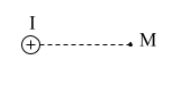
\includegraphics[scale=1]{../figs/VN11-2021-PH-TP021-01.JPG}
		\end{center}
		\begin{enumerate}[label=\alph*)]
			\item Hỏi điểm M cách dây một khoảng là bao nhiêu? 
			\item Biểu diễn vectơ cảm ứng từ tại điểm M.
		\end{enumerate}
		
	}
	
	\loigiai{
		
		\begin{enumerate}[label=\alph*)]
			\item  Khoảng cách từ M đến dây 
			
			$$B = 2 \cdot 10^{-7} \dfrac{I}{r} \Rightarrow r = \SI{0,05}{m}.$$
			
			\item Biểu diễn vectơ cảm ứng từ tại điểm M.
			\begin{center}
				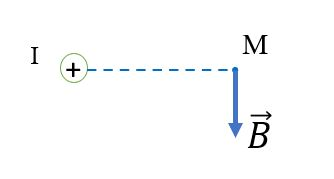
\includegraphics[scale=0.8]{../figs/VN11-2021-PH-TP021-05.JPG}
			\end{center}
			
		\end{enumerate}
	
	}
	
	

	
	\item \mkstar{3} [13]
	
	\cauhoi{
		\begin{minipage}[l]{12cm}
			Hai dây dẫn thẳng song song dài vô hạn đặt cách nhau một khoảng $\SI{14}{cm}$ trong không khí. Dòng điện chạy trong hai dây cùng chiều và có cường độ $I_1 = I_2 = \SI{2,5}{A}$. Đường thẳng CH nằm trong mặt phẳng vuông góc với mặt phẳng chứa hai dây dẫn và là đường trung trực của $I_1I_2$ (như hình vẽ) với  $\text{CH} = \SI{24}{cm}$.  Hãy vẽ vectơ cảm ứng từ tổng hợp tại C và tính độ lớn cảm ứng từ tổng hợp tại C.
		\end{minipage}
		\begin{minipage}[r]{5cm}
			\begin{center}
				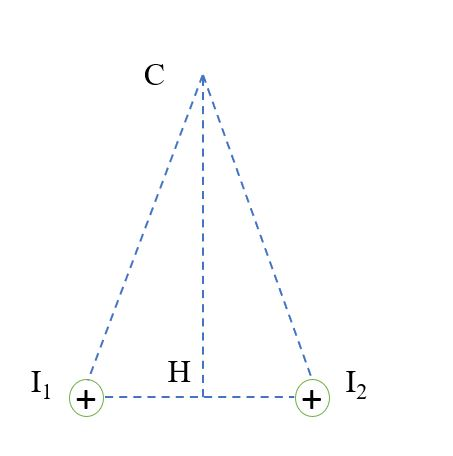
\includegraphics[scale=0.6]{../figs/VN11-2021-PH-TP021-02.JPG}
			\end{center}
		\end{minipage}
		
	}
	
	\loigiai{
		
		\begin{center}
			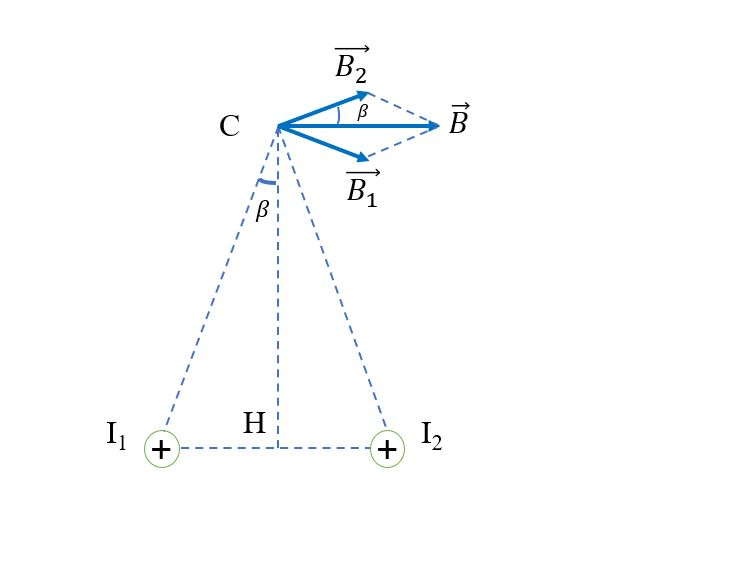
\includegraphics[scale=0.7]{../figs/VN11-2021-PH-TP021-03.JPG}
		\end{center}
		
		Ta có: $$ \vec B = \vec B_1 + \vec B_2.$$
		
		Do C là trung điểm của $I_1I_2$.
		
		Cảm ứng từ của $I_1$ và $I_2$ 
		
		$$B_1=B_2 = 2\cdot 10^{-7} \dfrac{I_1}{r_1} = 2 \cdot 10^{-6}\ \text{T}.$$
		
		Lại có: 
		
		$$\cos \beta = \dfrac{\text{CH}}{I_1\text{C}}.$$
		
		Cảm ứng từ tổng hợp 
		
		$$B=2B_1 \cos \beta= 3,84 \cdot 10^{-6}\ \text T.$$
		
	}
	\item \mkstar{3} [25]
	
	\cauhoi{
		
		Hai dây dẫn thẳng song song dài vô hạn đặt cách nhau $\SI{4}{cm}$ trong không khí. Dòng điện chạy trong hai dây là $I_1=\SI{10}{A}$; $I_2=\SI{20}{A}$ và ngược chiều nhau. Xác định hướng và độ lớn cảm ứng từ tại điểm M cách mỗi dây là $\SI{2}{cm}$.
		
		
	}
	\loigiai{
		
		\begin{center}
			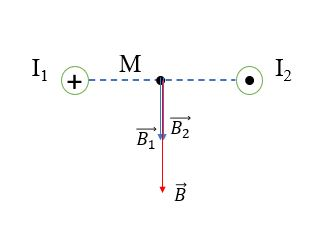
\includegraphics[scale=0.9]{../figs/VN11-2021-PH-TP021-04.JPG}
		\end{center}
		
		Cảm ứng từ của $I_1$ tác dụng lên M
		
		$$B_1 = 2 \cdot 10^{-7} \dfrac{I_1}{r_1} = 10^{-4}\ \text{T}.$$
		
		Cảm ứng từ của $I_2$ tác dụng lên M
		
		$$B_1 = 2 \cdot 10^{-7} \dfrac{I_1}{r_1} = 2 \cdot 10^{-4}\ \text{T}.$$
		
		Cảm ứng từ tổng hợp tại M
		
		$$ \vec B = \vec B_1 + \vec B_2$$
		
		Do $\vec B_1$ cùng hướng với $\vec B_2$ nên suy ra
		
		$$B = B_1+B_2 =3 \cdot 10^{-4}\ \text T.$$
		}
	
\end{enumerate}
\section{Lý thuyết: Từ trường do dòng điện chạy trong khung dây dẫn tròn hoặc trong ống dây hình trụ gây ra}
\begin{enumerate}[label=\bfseries Câu \arabic*:]
	
	\item \mkstar{2}
	
	\cauhoi{
		
		Khi cho dòng điện cường độ $\SI{10}{A}$ chạy qua một vòng dây dẫn đặt trong không khí thì cảm ứng từ tại tâm của vòng dây dẫn có độ lớn là $\text{2,1}\cdot 10^{-4}\ \text{T}$. Xác định bán kính của vòng dây.
		\begin{mcq}(4)
			\item $\SI{5,0}{cm}.$
			\item $\SI{0,3}{cm}.$
			\item $\SI{3,0}{cm}.$
			\item $\SI{2,5}{cm}.$
		\end{mcq}
	}
	\loigiai{
		
		\textbf{Đáp án: C.}
		
		Bán kính vòng dây  
		
		$$B = 2 \pi \cdot 10^{-7} \dfrac{I}{R} \Rightarrow R =  2 \pi \cdot 10^{-7} \dfrac{I}{B} = \SI{0,03}{m}.$$
	}	
	
	
	
		\item \mkstar{2}
		\cauhoi{
			
			Một vòng dây tròn đặt trong chân không có bán kính $R$ mang dòng điện có cường độ $I$ thì cảm ứng từ tại tâm vòng dây là $10\ \mu \text{T}$. Nếu cho dòng điện trên qua vòng dây có bán kính $4R$ thì cảm ứng từ tại tâm vòng dây có độ lớn là
			\begin{mcq}(4)
				\item $6 \cdot 10^{-6}\ \text{T}$.
				\item $\text{1,2}\cdot 10^{-6}\ \text{T}.$	
				\item $15 \cdot 10^{-6}\ \text{T}$.		
				\item $\text{2,5}\cdot 10^{-6}\ \text{T}.$	
			\end{mcq}
		}
		\loigiai{
			
			\textbf{Đáp án: D.}
			
			Ta có: 
			
			$$\dfrac{B_1}{B_2}= \dfrac{4R}{R} \Rightarrow B_2 = \dfrac{B_1}{4} =\text{2,5}\cdot 10^{-6}\ \text T. $$
		}	
	
		\item \mkstar{3}
		\cauhoi{
			
			Dùng một dây đồng có phủ một lớp sơn cách điện mỏng, quấn quanh một hình trụ dài $L = 50\ \text{cm}$, có đường kính $d = 4\ \text{cm}$ để làm một ống dây. Sợi dây quấn ống dây có chiều dài $l = 314\ \text{cm}$ và các vòng dây được quấn sát nhau. Hỏi nếu cho dòng điện cường độ $I = \text{0,4}\ \text{A}$ chạy qua ống dây, thì cảm ứng từ bên trong ống dây bằng bao nhiêu?
			\begin{mcq}(4)
				\item $5 \cdot 10^{-5}\ \text{T}$.			
				\item $\text{2,5}\cdot 10^{-5}\ \text{T}.$		
				\item $\text{1,25}\cdot 10^{-5}\ \text{T}.$		
				\item $3 \cdot 10^{-5}\ \text{T}$.	
			\end{mcq}
		}
		\loigiai{
			
			\textbf{Đáp án: B.}
			
			Chu vi của mỗi vòng dây $\pi d$.
			
			Số vòng dây
			
			$$N = \dfrac{l}{\pi d}.$$
			
			Cảm ứng từ tại bên trong ống dây
			
			$$B = 4 \pi \cdot 10^{-7} \dfrac{NI}{L}= 4  \cdot 10^{-7} \dfrac{ lI}{Ld} = \text{2,5} \cdot 10^{-5}\ \text{T}.$$
		}	

	
		\item \mkstar{1} [19]
	
	\cauhoi{
		
		Nêu công thức tính cảm ứng từ tại tâm của một khung dây dẫn tròn đặt trong không khí (có chú thích các đại lượng trong công thức).
		
	}
	
	\loigiai{
		
		+ Biểu thức: $$B = 2\pi \cdot 10^{-7} N \dfrac{I}{R}$$
		
		$N$: số vòng dây của khung.
		
		$I$: cường độ dòng điện qua khung.
		
		$R$: bán kính khung dây.
		
	}
\end{enumerate}

\whiteBGstarEnd
	\stopcontents[mychapters]
	
\setcounter{mychapter}{21}
	\mychapter{Lực Lo-ren-xơ}
	\startcontents[mychapters]
	\printcontents[mychapters]{}{0}{\setcounter{tocdepth}{1}}
	\whiteBGstarBegin
\setcounter{section}{0}
\section{Lý thuyết: Lực Lo-ren-xơ }
\begin{enumerate}[label=\bfseries Câu \arabic*:]
	\item \mkstar{2} 
	
	\cauhoi{
		Cho electron bay vào miền có từ trường đều với vận tốc $v = 8\cdot 10^5\ \text{m/s}$ theo phương vuông góc với vectơ cảm ứng từ, độ lớn cảm ứng từ là $B = \text{9,1}\cdot 10^{-4}\ \text{T}$. Tính độ lớn lực Lo-ren-xơ tác dụng lên electron.
		\begin{mcq}(2)
			\item $\text{1,1648}\cdot 10^{-16}\ \text{N}$. 
			\item $\text{1,1648}\cdot 10^{-17}\ \text{N}$.
			\item $\text{1,1648}\cdot 10^{-19}\ \text{N}$.
			\item $\text{1,1648}\cdot 10^{-20}\ \text{N}$.
		\end{mcq}
	}
	
	\loigiai{
		\textbf{Đáp án: A.}
		
		Góc hợp bởi $\vec B$ và $\vec v$ là $90^\circ$ nên ta có độ lớn của lực Lorenxo: 
		
		$$f = |e|vB \sin \alpha = 1,1648 \cdot 10^{-16}\ \text N.$$
		
	}
	\item \mkstar{2} 
	
	\cauhoi{
		Một hạt mang điện $\text{3,2}\cdot 10^{-19}\ \text{C}$ bay vào trong từ trường đều có $B = \text{0,5}\ \text{T}$ hợp với hướng của đường sức từ $30^\circ$. Lực Lorenxơ tác dụng lên hạt có độ lớn $\text{8}\cdot 10^{-14}\ \text{N}$. Vận tốc của hạt đó khi bắt đầu vào trong từ trường là bao nhiêu?
		\begin{mcq}(2)
			\item $v = 2\cdot 10^6\ \text{m/s}$.
			\item $v = 1\cdot 10^6\ \text{m/s}$.
			\item $v = 3\cdot 10^6\ \text{m/s}$.
			\item $v = 5\cdot 10^6\ \text{m/s}$.
		\end{mcq}
		
	}
	
	\loigiai{
		\textbf{Đáp án: B.}
		
		Vận tốc của hạt đó khi bắt đầu vào trong từ trường 
		
		$$f =qvB \sin  \alpha \Rightarrow v = \dfrac{F}{|q| B \sin \alpha} = 10^6\ \text{m/s}.$$
	}
	
		\item \mkstar{3} 
	
	\cauhoi{
		Một hạt điện tích chuyên động trong từ trường đều quĩ đạo của hạt vuông góc với đường sức từ. Nếu hạt chuyển động với vận tốc $v_1=\text{1,8}\cdot 10^{6}\ \text{m/s}$ thì lực Lo-ren-xơ tác dụng lên hạt có độ lớn là $f_1=\text{2}\cdot 10^{-6}\ \text{N}$, nếu hạt chuyển động với vận tốc là $v_1=\text{4,5}\cdot 10^{7}\ \text{m/s}$ thì lực Loren tác dụng lên hạt có giá trị là
		\begin{mcq}(2)
			\item $f_2=\text{2}\cdot 10^{-5}\ \text{N}$. 
			\item $f_2=\text{3}\cdot 10^{-5}\ \text{N}$.
			\item $f_2=\text{5}\cdot 10^{-5}\ \text{N}$.
			\item $f_2=\text{6}\cdot 10^{-5}\ \text{N}$.
		\end{mcq}
	}
	
	\loigiai{
		\textbf{Đáp án: C.}
		
		Một hạt tích điện chuyển động trong từ trường đều, lực Lorenxo tác dụng lên hạt 
		
		$$f_1 = qvB_1.$$ 
		
		$$f_2 = qvB_2.$$
		
		Ta có: 
		
		$$\dfrac{f_2}{f_1} = \dfrac{v_2}{v_1} \Leftrightarrow \dfrac{f_2}{2 \cdot 10^{-6}} = \dfrac{4,5 \cdot 10^7}{1,8 \cdot 10^6} \Rightarrow f_2 = 5 \cdot 10^{-5}\ \text{N}.$$
			
	}
	
	
\end{enumerate}
\section{Lý thuyết: Chuyển động của hạt mang điện trong từ trường đều (đọc thêm)}
\begin{enumerate}[label=\bfseries Câu \arabic*:]
		\item \mkstar{2}
	
	\cauhoi{
		Một ion bay theo quỹ đạo hòn bán kính $R$ trong một mặt phẳng vuông góc với các đường sức của một từ trường đều. Khi độ lớn vận tốc tăng gấp đôi thì bán kính quỹ đạo là 
		\begin{mcq}(4)
			\item $\dfrac{R}{2}.$ 
			\item $\dfrac{R}{4}.$
			\item $2R.$
			\item $4R.$
		\end{mcq}
		
	}
	
	\loigiai{
		\textbf{Đáp án: C.}
		
		Bán kính quỹ đạo của ion chuyển động trong từ trường khi có vận tốc vuông góc với đường sức từ là: 
		
		$$R = \dfrac{mv}{|q|B}.$$
		
		Vậy khi vận tốc tăng lên gấp đôi thì bán kính cũng tăng lên 2 lần.
	}
	
	\item \mkstar{3}
	\cauhoi{
		Hạt electron với vận tốc đầu bằng không được gia tốc qua một hiệu điện thế $\SI{400}{V}$. Tiếp đó nó được dẫn vào miền có từ trường đều vuông góc hướng chuyển động. Quỹ đạo của electron là đường tròn bán kính $R = \SI{7}{cm}$. Xác định độ lớn cảm ứng từ $B$.
		\begin{mcq}(2)
			\item $\text{9,636}\cdot 10^{-4}\ \text{T}$.
			\item $\text{4,818}\cdot 10^{-4}\ \text{T}$.
			\item $\text{3,212}\cdot 10^{-4}\ \text{T}$.
			\item $\text{6,242}\cdot 10^{-4}\ \text{T}$.
		\end{mcq}
	}
	
	\loigiai{
		\textbf{Đáp án: A.}
		
		Độ biến thiên động năng bằng công ngoại lực.
		
		Vận tốc của electron thu được khi tăng tốc bằng hiệu điện thế $U$ là
		
		$$\dfrac{1}{2} m_e v^2 =|e|U \Rightarrow v = 1,186 \cdot 10^7\ \text{m/s}.$$
		
		Khi electron đi vào từ trường đều, lực Lorenxo đóng vai trò là lực hướng tâm 
		
		$$|e| vB = \dfrac{m_e v^2}{r} \Rightarrow B = 9,636 \cdot 10^{-4}\ \text{T}.$$
	}


\end{enumerate}

\whiteBGstarEnd
	\stopcontents[mychapters]
	
\chapter[\textbf{Ôn tập: Chương IV. Từ trường}]{Ôn tập: Chương IV. Từ trường}
	\startcontents[chapters]
	\printcontents[chapters]{}{0}{\setcounter{tocdepth}{1}}
	\whiteBGstarBegin
\setcounter{section}{0}
\section{Trắc nghiệm}
\begin{enumerate}[label=\bfseries Câu \arabic*:]
	
	
	\item \mkstar{1}
	
	\cauhoi
	{Người ta gọi silic là chất bán dẫn vì
		\begin{mcq}
			\item nó không phải là kim loại, cũng không phải là điện môi.
			\item hạt tải điện trong đó có thể là electron và lỗ trống.
			\item điện trở suất của nó rất nhạy với nhiệt độ, tạp chất và các tác nhân ion khác.
			\item Cả 3 lí do trên.
		\end{mcq}
		
	}
	\loigiai
	{	\textbf{Đáp án: D.}
		
	}
	\item \mkstar{1}
	
	\cauhoi
	{Phát biểu nào dưới dây về transistor là chính xác?
		\begin{mcq}
			\item Một bán dẫn loại p kẹp giữa hai lớp bán dẫn loại n là transistor n-p-n.
			\item Một bán dẫn loại n mỏng kẹp giữa hai lớp bán dẫn loại p không thể xem là transistor.
			\item Một lớp bán dẫn loại p mỏng kẹp giữa hai lớp bán dẫn loại n luôn có khả năng là mạch khuếch đại.
			\item Trong transistor n-p-n, bao giờ mật độ hạt tải điện vùng Emitor cũng cao hơn vùng Base.
		\end{mcq}
		
	}
	\loigiai
	{	\textbf{Đáp án: D.}
	
	}
	\item \mkstar{1}
	
	\cauhoi
	{Silic tinh khiết thì
		\begin{mcq}
			\item dẫn điện tốt ở moi nhiệt độ.
			\item chỉ dẫn điện tốt khi ở nhiệt độ thấp.
			\item có liên kết đồng hóa trị giữa hai nguyên tử.
			\item chỉ có một loại hạt tải điện là electron.
		\end{mcq}
		
	}
	\loigiai
	{	\textbf{Đáp án: C.}
		
	}
	\item \mkstar{1}
	
	\cauhoi
	{Pin mặt trời là một nguồn điện biến đổi năng lượng từ
		\begin{mcq}(2)
			\item nhiệt năng thành điện năng.
			\item quang năng thành điện năng.
			\item cơ năng thành điện năng.
			\item hóa năng thành điện năng.
		\end{mcq}
		
	}
	\loigiai
	{	\textbf{Đáp án: B.}
		
	}
	\item \mkstar{1}
	
	\cauhoi
	{Lớp tiếp giáp p-n có
		\begin{mcq}
			\item tác dụng ngăn cản các electron từ p sang n.
			\item tác dụng ngăn cản các electron từ n sang p.
			\item tính dẫn điện một chiều từ n sang p.
			\item tính dẫn điện một chiều từ p sang n.
		\end{mcq}
		
	}
	\loigiai
	{	\textbf{Đáp án: C.}
		
	}
	\item \mkstar{1}
	
	\cauhoi
	{Cách pha tạp nào sau đây tạo ra bán dẫn loại p?
		\begin{mcq}(2)
			\item Si pha tạp As.
			\item Si pha tạp B.
			\item Si pha tạp S.
			\item Si pha tạp Pb.
		\end{mcq}
		
	}
	\loigiai
	{	\textbf{Đáp án: B.}
		
	}
	\item \mkstar{1}
	
	\cauhoi
	{Hạt mang điện chủ yếu trong bán dẫn loại n là
		\begin{mcq}(2)
			\item lỗ trống.
			\item electron.
			\item electron và lỗ trống.
			\item electron và ion dương.
		\end{mcq}
		
	}
	\loigiai
	{	\textbf{Đáp án: B.}
		
	}
	\item \mkstar{1}
	
	\cauhoi
	{Chọn câu đúng. Diode bán dẫn được dùng để
		\begin{mcq}
			\item nấu chảy kim loại.
			\item chỉnhh lưu dòng điện xoay chiều.
			\item tạo ra dòng điện xoay chiều.
			\item biến đổi dòng điện một chiều thành dòng điện xoay chiều.
		\end{mcq}
		
	}
	\loigiai
	{	\textbf{Đáp án: B.}
		
	}
	\item \mkstar{1}
	
	\cauhoi
	{Bán dẫn chứa tạp chất nhận là bán dẫn có đặc điểm:
		\begin{mcq}
			\item có mật độ lỗ trống rất lớn so với mật độ electron.
			\item có mật độ electron rất lớn so với mật độ lỗ trống.
			\item chỉ có một loại hạt tải điện là lỗ trống.
			\item chỉ có một loại hạt tải điện là electron.
		\end{mcq}
		
	}
	\loigiai
	{	\textbf{Đáp án: A.}
		
	}
	\item \mkstar{1}
	
	\cauhoi
	{Transistor là dụng cụ bán dẫn có số lớp chuyển tiếp p-n trong nó là
		\begin{mcq}(4)
			\item 4 lớp.
			\item 2 lớp.
			\item 3 lớp .
			\item 1 lớp.
		\end{mcq}
		
	}
	\loigiai
	{	\textbf{Đáp án: B.}
		
	}

\end{enumerate}

\whiteBGstarEnd

\loigiai
{
	\begin{center}
		\textbf{BẢNG ĐÁP ÁN}
	\end{center}
	\begin{center}
		\begin{tabular}{|m{2.8em}|m{2.8em}|m{2.8em}|m{2.8em}|m{2.8em}|m{2.8em}|m{2.8em}|m{2.8em}|m{2.8em}|m{2.8em}|}
			\hline
			1.D  & 2.D  & 3.C  & 4.B  & 5.C  & 6.B  & 7.B  & 8.B  & 9.A  & 10.B  \\
			\hline
			
		\end{tabular}
	\end{center}
}
\section{Tự luận}
\begin{enumerate}[label=\bfseries Câu \arabic*:]
	\item \mkstar{1}
	
	\cauhoi{
		Chất bán dẫn là gì? Nêu bản chất dòng điện trong chất bán dẫn.
	}
	
	\loigiai{
		
		Chất bán dẫn là chất có điện trở suất nằm trong khoảng trung gian giữa kim loại và chất điện môi.
		
		Dòng điện trong chất bán dẫn là dòng các electron dẫn chuyển động ngược chiều điện trường và dòng các lỗ trống chuyển động cùng chiều điện trường.
	}
	
	\item \mkstar{2}
	
	\cauhoi{
		So sánh chất bán dẫn loại n và loại p theo các tiêu chí được cho trong bảng sau:
		\begin{longtable}{|m{8em}|m{14em}|m{14em}|}
			\hline
			& \thead{Bán dẫn loại n} & \thead{Bán dẫn loại p} \\
			\hline
			\textbf{Định nghĩa} & & \\
			\hline
			\textbf{Hạt tải đa số} & & \\
			\hline
			\textbf{Tạp chất} & & \\
			\hline
		\end{longtable}
	}
	
	\loigiai{
		
		\begin{longtable}{|m{8em}|m{14em}|m{14em}|}
			\hline
			& \thead{Bán dẫn loại n} & \thead{Bán dẫn loại p} \\
			\hline
			\textbf{Định nghĩa} & Là chất bán dẫn mà hạt tải điện đa số trong đó mang điện âm. & Là chất bán dẫn mà hạt tải điện đa số trong đó mang điện dương.\\
			\hline
			\textbf{Hạt tải đa số} & Các electron. & Các lỗ trống. \\
			\hline
			\textbf{Tạp chất} & Tạp chất cho (donor): Sinh ra electron dẫn, thường là những nguyên tố có 5 electron hóa trị như $\ce{P}$, $\ce{As}$, $\ldots$. & Tạp chất nhận (aceptor): Nhận electron (đồng nghĩa sinh ra lỗ trống), thường là những nguyên tố có 5 electron hóa trị như $\ce{B}$, $\ce{Al}$, $\ldots$.\\
			\hline
		\end{longtable}
	}
	\item \mkstar{3}
	
	\cauhoi{
		Ở nhiệt độ phòng, trong bán dẫn Si tinh khiết có số cặp điện tử-lỗ trống bằng $\SI{e-13}{}$ lần số nguyên tử Si. Tìm số cặp điện tử-lỗ trống có trong $\SI{2}{mol}$ nguyên tử Si.
	}
	
	\loigiai{
		
		Số nguyên tử $\ce{Si}$ có trong $\SI{2}{\mol}$ là
		$$N = 2 N_\text{A} = \SI{1.205e24}{}.$$
		
		Số cặp điện tử-lỗ trống bằng $\SI{e-13}{}$ lần số nguyên tử, suy ra số cặp điện tử-lỗ trống là
		$$\SI{e-13}{} \cdot N = \SI{1.205e11}{}.$$
	}
	\item \mkstar{3}
	
	\cauhoi{
		Ở nhiệt độ phòng, trong bán dẫn Si tinh khiết có số cặp điện tử-lỗ trống bằng $\SI{e-13}{}$ lần số nguyên tử Si. Nếu pha P và Si với tỉ lệ một phần triệu thì số hạt tải điện tăng lên bao nhiêu lần?
	}
	
	\loigiai{
		
		Gọi $N_0$ là số nguyên tử $\ce{Si}$ có trong chất bán dẫn.
		
		Ở nhiệt độ phòng, trong bán dẫn $\ce{Si}$ tinh khiết, số cặp điện tử-lỗ trống bằng $\SI{e-13}{} N_0$. Tức là số hạt tải điện bằng:
		$$N=\SI{e-13}{} N_0.$$
		
		Khi pha một nguyên tử $\ce{P}$ vào bán dẫn $\ce{Si}$ tinh khiết sẽ tạo ra thêm 1 electron tự do. Với tỉ lệ pha tạp là một phần triệu thì số hạt tải điện tăng thêm là
		$$\Delta N = \SI{e-6}{} N_0.$$
		
		Vậy số hạt tại điện tăng thêm gấp $\dfrac{\Delta N}{N} = \SI{5e6}{}$ lần.
	}
	
\end{enumerate}
	\stopcontents[chapters]
	
\setcounter{mychapter}{22}
	\mychapter{Từ thông. Cảm ứng điện từ}
	\startcontents[mychapters]
	\printcontents[mychapters]{}{0}{\setcounter{tocdepth}{1}}
	\whiteBGstarBegin
\setcounter{section}{0}
\section{Trắc nghiệm}
\begin{enumerate}[label=\bfseries Câu \arabic*:]
	
	
	\item \mkstar{1}
	
	\cauhoi
	{Câu nào dưới đây nói về chất điện phân là \textbf{không} đúng?
		\begin{mcq}
			\item Chất điện phân khi có dòng điện chạy qua sẽ giải phóng các chất ở các điện cực.
			\item Trong dung dịch, các phân tử axit, muối, bazơ đều bị phân li thành các ion.
			\item Một số chất rắn khi nóng chảy cũng là chất điện phân.
			\item Chất điện phân nhất thiết phải là dung dịch của các chất tan được trong dung môi.
		\end{mcq}
		
	}
	\loigiai
	{	\textbf{Đáp án: D.}
		
		Chất điện phân không nhất thiết phải là dung dịch của các chất tan được trong dung môi.
	}
	\item \mkstar{1}

\cauhoi
{Câu nào sau đây khi nói về dòng điện trong chất điện phân là đúng?
	\begin{mcq}
		\item Khi có dòng điện chạy qua bình điện phân thì các electron và ion âm đi về phía anode, còn các ion dương đi về cathode.
		\item Khi có dòng điện chạy qua bình điện phân thì các electron đi về phía anode, các ion dương đi về cathode.
		\item Khi có dòng điện chạy qua bình điện phân thì các ion âm đi về phía anode, các ion dương đi về cathode.
		\item Khi có dòng điện chạy qua bình điện phân thì các ion âm và electron đi về phía cathode, các ion dương đi về anode.
	\end{mcq}
	
}
\loigiai
{	\textbf{Đáp án: C.}
	
	Khi có dòng điện chạy qua bình điện phân thì các ion âm đi về phía anode, các ion dương đi về cathode.
}
	\item \mkstar{1}

\cauhoi
{Câu phát biểu nào sau đây \textbf{sai}?
	\begin{mcq}
		\item Dòng điện trong kim loại là dòng chuyển dời có hướng của các electron ngược chiều điện trường.
		\item Dòng điện trong chất điện phân là dòng chuyển dời có hướng của các ion dương theo chiều điện trường, của các ion âm ngược chiều điện trường.
		\item Dòng điện trong chất khí là dòng chuyển dời có hướng của các ion dương theo chiều điện trường, của các ion âm ngược chiều điện trường.
		\item Dòng điện trong chân không là dòng chuyển dời có hướng của các electron phát xạ từ cathode bị nung nóng dưới tác dụng của điện trường.
	\end{mcq}
	
}
\loigiai
{	\textbf{Đáp án: C.}
	
	Dòng điện trong chất khí là dòng chuyển dời có hướng của các ion dương theo chiều điện trường, của các ion âm và các electron ngược chiều điện trường. Các hạt tải điện này là do chất khí bị ion hóa sinh ra.
}
	\item \mkstar{1}

\cauhoi
{Câu nào sau đây \textbf{sai} khi nói về tính dẫn điện của chất điện phân?
	\begin{mcq}
		\item Dòng điện trong chất điện phân tuân theo định luật Ôm.
		\item Độ dẫn điện của chất điện phân tăng khi nhiệt độ tăng.
		\item Điện trở của chất điện phân giảm khi nhiệt độ tăng.
		\item Khi ắc quy được nạp điện, dòng điện qua ắc quy cũng là dòng điện trong chất điện phân.
	\end{mcq}
	
}
\loigiai
{	\textbf{Đáp án: A.}
	
	Dòng điện trong chất điện phân chỉ tuân theo định luật Ôm khi xảy ra hiện tượng dương cực tan.
}
	\item \mkstar{2}

\cauhoi
{Phát biểu nào sau đây là đúng?
	\begin{mcq}
		\item Dòng điện trong kim loại cũng như trong chân không đều là dòng chuyển động có hướng của các electron, ion dương và ion âm.
		\item Dòng điện trong kim loại là dòng chuyển động có hướng của các electron, dòng điện trong chân không và trong chất khí đều là dòng chuyển động có hướng của các ion dương và ion âm.
		\item Dòng điện trong kim loại và trong chân không đều là dòng chuyển động có hướng của các electron.
		\item Dòng điện trong kim loại và dòng điện trong chất khí là dòng chuyển động có hướng của các ion.
	\end{mcq}
	
}
\loigiai
{	\textbf{Đáp án: C.}
	
	Dòng điện trong kim loại và trong chân không đều là dòng chuyển động có hướng của các electron.
}
	\item \mkstar{2}

\cauhoi
{Nguyên nhân gây ra điện trở của kim loại là
	\begin{mcq}
		\item do sự va chạm của các electron với các ion dương ở các nút mạng.
		\item do sự va chạm của các ion dương ở các nút mạng với nhau.
		\item do sự va chạm của các electron với nhau.
		\item Cả B và C đều đúng.
	\end{mcq}
	
}
\loigiai
{	\textbf{Đáp án: A.}
	
	Nguyên nhân gây ra điện trở của kim loại là do sự va chạm của các electron với các ion dương ở các nút mạng.
}
	\item \mkstar{2}

\cauhoi
{Phát biểu nào dưới đây về sự phụ thuộc của cường độ dòng điện $I$ vào hiệu điện thế $U$ giữa hai cực tụ điện chứa chất khí trong quá trình dẫn điện không tự lực là \textbf{không} đúng?
	\begin{mcq}
		\item Với mọi giá trị của $U$, $I$ luôn tăng tỉ lệ với $U$.
		\item Với $U$ nhỏ, $I$ tăng theo $U$.
		\item Với $U$ đủ lớn, $I$ đạt giá trị bão hòa.
		\item Với $U$ quá lớn, $I$ tăng nhanh theo $U$.
	\end{mcq}
	
}
\loigiai
{	\textbf{Đáp án: A.}
	
	Dòng điện $I$ tỉ lệ với $U$ đến khi $I$ đạt bão hòa thì $I$ không tăng nữa. Khi đó $I$ không còn tỉ lệ với $U$.
}
	\item \mkstar{2}

\cauhoi
{Hai thanh kim loại được nối với nhau bởi hai đầu mối hàn tạo thành một mạch kín, hiện tượng nhiệt điện chỉ xảy ra khi
	\begin{mcq}
		\item hai thanh kim loại có bản chất khác nhau và nhiệt độ ở hai đầu mối hàn bằng nhau.
		\item hai thanh kim loại có bản chất khác nhau và nhiệt độ ở hai đầu mối hàn khác nhau.
		\item hai thanh kim loại có bản chất giống nhau và nhiệt độ ở hai đầu mối hàn bằng nhau.
		\item hai thanh kim loại có bản chất giống nhau và nhiệt độ ở hai đầu mối hàn khác nhau.
	\end{mcq}
	
}
\loigiai
{	\textbf{Đáp án: B.}
	
	Hai thanh kim loại được nối với nhau bởi hai đầu mối hàn tạo thành một mạch kín, hiện tượng nhiệt điện chỉ xảy ra khi hai thanh kim loại có bản chất khác nhau và nhiệt độ ở hai đầu mối hàn khác nhau.
}
	\item \mkstar{2}

\cauhoi
{Khi cho dòng điện chạy qua một sợi dây thép có hệ số nhiệt điện trở là $\SI{0.004}{K^{-1}}$ thì điện trở của nó tăng gấp đôi. Nhiệt độ của sợi dây này đã tăng thêm
	\begin{mcq}(4)
		\item $\SI{800}{\celsius}$.
		\item $\SI{250}{\celsius}$.
		\item $\SI{300}{\celsius}$.
		\item $\SI{80}{\celsius}$.
	\end{mcq}
	
}
\loigiai
{	\textbf{Đáp án: B.}
	
	Áp dụng công thức:
	$$R=R_0 [1+ \alpha (t-t_0)] \Rightarrow t-t_0 = \SI{250}{\celsius}.$$
}
	\item \mkstar{2}

\cauhoi
{Ở $\SI{20}{\celsius}$, điện trở suất của bạc là $\SI{1.62e-8}{\Omega m}$. Biết hệ số nhiệt điện trở của bạc là $\SI{4.1e-3}{K^{-1}}$. Ở $\SI{330}{K}$ thì điện trở suất của bạc là
	\begin{mcq}(2)
		\item $\SI{1.866e-8}{\Omega m}$.
		\item $\SI{3.679e-8}{\Omega m}$.
		\item $\SI{3.812e-8}{\Omega m}$.
		\item $\SI{4.151e-8}{\Omega m}$.
	\end{mcq}
	
}
\loigiai
{	\textbf{Đáp án: A.}
	
	Ta có $t-t_0 = \SI{330}{K} - \SI{293}{K} = \SI{37}{K}$.
	
	Áp dụng công thức:
	$$\rho = \rho_0 [1+ \alpha (t-t_0)] = \SI{1.866e-8}{\Omega m}.$$
}
	
\end{enumerate}

\whiteBGstarEnd

\loigiai
{
	\begin{center}
		\textbf{BẢNG ĐÁP ÁN}
	\end{center}
	\begin{center}
		\begin{tabular}{|m{2.8em}|m{2.8em}|m{2.8em}|m{2.8em}|m{2.8em}|m{2.8em}|m{2.8em}|m{2.8em}|m{2.8em}|m{2.8em}|}
			\hline
			1.D  & 2.C  & 3.C  & 4.A  & 5.C  & 6.A  & 7.A  & 8.B  & 9.B  & 10.A  \\
			\hline
			
		\end{tabular}
	\end{center}
}
\section{Tự luận}
\begin{enumerate}[label=\bfseries Câu \arabic*:]
	\item \mkstar{2}
	
	\cauhoi{
	Một sợi dây đồng có điện trở $\SI{74}{\Omega}$ ở $\SI{50}{\celsius}$, có hệ số nhiệt điện trở là $\SI{4.1e-3}{K^{-1}}$. Tính điện trở của sợi dây đó ở $\SI{100}{\celsius}$.
	}
	
	\loigiai{
		
		Điện trở của sợi dây ở $\SI{100}{\celsius}$:
		$$\dfrac{R_2}{R_1} = \dfrac{1 + \alpha t_2}{1+ \alpha t_1} \Rightarrow R_2 = \SI{86.6}{\Omega}.$$
	}
	
	\item \mkstar{2}
	
	\cauhoi{
		Một mối hàn của một cặp nhiệt điện có hệ số $\alpha_T = \SI{48}{\micro V / K}$ được đặt trong không khí ở $\SI{20}{\celsius}$, còn mối hàn kia được nung nóng đến nhiệt độ $t \SI{}{\celsius}$, suất điện động của cặp nhiệt điện khi đó là $\calE = \SI{6}{mV}$. Xác định nhiệt độ của mối hàn còn lại.
	}
	
	\loigiai{
		
		Áp dụng công thức tính suất điện động nhiệt điện:
		$$\calE = \alpha_T (T_1 - T_2) \Rightarrow T_1 = \SI{418}{K} \Rightarrow t_1 = \SI{145}{\celsius}.$$
	}
	\item \mkstar{2}
	
	\cauhoi{
		Một bình điện phân chứa dung dịch bạc nitrate có điện trở là $\SI{5}{\Omega}$. Anode của bình bằng bạc và hiệu điện thế đặt vào hai điện cực của bình là $\SI{20}{V}$. Tính khối lượng bạc bám vào cathode sau 32 phút 10 giây.
	}
	
	\loigiai{
		
		Cường độ dòng điện qua bình điện phân:
		$$I=\dfrac{U}{R} = \SI{4}{A}.$$
		
		Áp dụng định luật Fa-ra-đây để tính khối lượng bạc bám vào cathode:
		$$m=\dfrac{1}{F} \dfrac{A}{n} I t = \SI{8.64}{g}.$$
	}
	\item \mkstar{3}
	
	\cauhoi{
		Để giải phóng lượng $\ce{Cl}$ và $\ce{H}$ từ $\SI{7.6}{g}$ $\ce{HCl}$ bằng dòng điện $\SI{5}{A}$ thì phải cần thời gian điện phân là bao lâu? Biết rằng đương lượng điện của $\ce{H}$ và $\ce{Cl}$ lần lượt là $k_1=\SI{0.1045e-7}{kg/C}$ và $k_2 = \SI{3.6e-7}{kg/C}$.
	}
	
	\loigiai{
		
		Áp dụng định luật Fa-ra-đây:
		$$m=(k_1 + k_2) It$$
		
		Suy ra thời gian cần phải điện phân là
		$$t=\SI{4027}{s} \approx \SI{1.1}{h}.$$
	}
	
\end{enumerate}
	\stopcontents[mychapters]
	
\setcounter{mychapter}{23}
	\mychapter{Suất điện động cảm ứng}
	\startcontents[mychapters]
	\printcontents[mychapters]{}{0}{\setcounter{tocdepth}{1}}
	\whiteBGstarBegin
\setcounter{section}{0}

\begin{enumerate}[label=\bfseries Câu \arabic*:]
	
		\item \mkstar{1} [21]
		
		\cauhoi{
			Độ lớn của suất điện động cảm ứng trong mạch kín tỉ lệ với 
			
			\begin{mcq}
				\item tốc độ biến thiên từ thông qua mạch ấy.	 
				\item độ lớn từ thông qua mạch.
				\item điện trở của mạch.	
				\item diện tích của mạch.
			\end{mcq}
		}
		
		\loigiai{
			\textbf{Đáp án: A.}
			
			Độ lớn của suất điện động cảm ứng trong mạch kín tỉ lệ với tốc độ biến thiên từ thông qua mạch ấy.
		}
	
			\item \mkstar{1} [21]
		
		\cauhoi{
			Độ lớn của suất điện động cảm ứng trong một mạch kín được xác định theo công thức
			
			\begin{mcq}(2)
				\item  $e_\text c = \left|\dfrac{\Delta \Phi}{\Delta t}\right|$.
				\item  $e_\text c = |\Delta \Phi \cdot \Delta t|$.
				\item  $e_\text c = \left|\dfrac{\Delta t}{\Delta \Phi}\right|$.
				\item  $e_\text c = - \left|\dfrac{\Delta \Phi}{\Delta t}\right|$.
			\end{mcq}
		}
		
		\loigiai{
			\textbf{Đáp án: A.}
			
			Độ lớn của suất điện động cảm ứng trong một mạch kín được xác định theo công thức
			$$e_\text c = \left|\dfrac{\Delta \Phi}{\Delta t}\right|.$$
			
		}
	
		\item \mkstar{1} [7]
	
	\cauhoi{
		
		Phát biểu định luật Faraday. Viết công thức của định luật.
		
	}
	
	\loigiai{
		
		Độ lớn của suất điện động cảm ứng xuất hiện trong mạch kín tỉ lệ với tốc độ biến thiên từ thông qua mạch kín đó.
		
		$$|e_\text c|= \left|-\dfrac{\Delta \Phi}{\Delta t}\right|.$$
		
	}

	\item \mkstar{1} [35]
	
	\cauhoi{
		
		Suất điện động cảm ứng là gì? Phát biểu, viết công thức, ghi tên, đơn vị các đại lượng trong công thức của định luật Fa-ra-đây về hiện tượng cảm ứng điện từ.
		
		Vận dụng: Một khung dây phẳng diện tích $\SI{20}{cm}^2$, gồm $10$ vòng dây đặt trong từ trường đều, góc giữa $\vec B$ và mặt phẳng khung dây là $30^\circ$, $B = 4\cdot 10^{-4}\ \text T$, làm cho từ trường giảm đều về $0$ trong thời gian $\SI{0,01}{s}$. Hãy xác định độ lớn của suất điện động cảm ứng sinh ra trong khung dây.
		
		
		
	}
	
	\loigiai{
		
		Định nghĩa:
	
	Suất điện động cảm ứng là suất điện động sinh ra dòng điện cảm ứng trong mạch kín. 
	
	Định luật Fa-ra-đây về hiện tượng cảm ứng điện từ 
	
	- Phát biểu: “Độ lớn của suất điện động cảm ứng xuất hiện trong mạch kín tỉ lệ với tốc độ biến thiên từ thông qua mạch kín đó” 
	- Công thức suất điện động cảm ứng:
	
	$$e_\text c = -\dfrac{\Delta \Phi}{\Delta t}$$
	
	- Độ lớn:
	
	$$|e_\text c| = \left|-\dfrac{\Delta \Phi}{\Delta t}\right|$$
	
	trong đó:
	
	+ $\left|\dfrac{\Delta \Phi}{\Delta t}\right|$: tốc độ biến thiên từ thông (Wb/s).
	
	+ $e_\text c$: suất điện động cảm ứng (V)  
	
	Vận dụng: Suất điện động cảm ứng trong khung:($\alpha = 90^\circ - 30^\circ = 60^\circ$) 
	
	$$e_\text{c} = -\dfrac{\Delta \Phi}{\Delta t} =- \dfrac{N\Delta B S \cos \alpha}{\Delta t}= 4 \cdot 10^{-4}\ \text{V}.$$
	
		
	}

	\item \mkstar{2} [34]
	
	\cauhoi{
		
		Một khung dây phẳng, tròn, bán kính $\SI{0,1}{m}$, có $100$ vòng dây, đặt trong từ trường đều. Mặt phẳng khung dây vuông góc với các đường cảm ứng từ. Lúc đầu cảm ứng từ có giá trị $\SI{0,2}{T}$. Xác định độ lớn suất điện động cảm ứng trong cuộn dây nếu trong $\SI{0,2}{s}$ cảm ứng từ tăng đều lên gấp ba.
		
		
	}
	\loigiai{
		
	Độ biến thiên từ thông 
	
	$$\Delta \Phi = N \Delta BS \cos 0^\circ = \pi \dfrac{2}{5}\ \text{Wb}.$$
	
	Suất điện động cảm ứng trong cuộn dây
	
	$$|e_\text c| = \left|\dfrac{\Delta \Phi}{\Delta t}\right| = \pi \ \text V.$$ 

	
	}

	
	\item \mkstar{2} [10]
	
	\cauhoi{
		
		Một khung dây phẳng diện tích $\SI{20}{cm}^2$ gồm $10$ vòng dây, được đặt trong từ trường đều có vectơ cảm ứng từ hợp với mặt phẳng khung dây một góc $30^\circ$ và có độ lớn $2\cdot 10^{-4}\ \text T$. Người ta cho từ trường qua khung dây giảm đều đến không trong $\SI{0,01}{s}$. Tính độ lớn suất điện động cảm ứng xuất hiện trong thời gian từ trường biến đổi.
		
		
	}
	\loigiai{
		
		Độ lớn suất điện động cảm ứng xuất hiện trong thời gian từ trường biến đổi
		
		$$|e_\text c|= \left|-\dfrac{N\Delta B S \cos \alpha}{\Delta t}\right|= 2 \cdot 10^{-4}\ \text{V}.$$
	}

	\item \mkstar{3} [14]
	
	\cauhoi{
		Một khung dây gồm $500$ vòng dây, diện tích mỗi vòng $\SI{10}{cm}^2$, khung đặt trong từ trường đều. Cảm ứng từ  hợp với mặt phẳng khung dây góc $30^\circ$  và có độ lớn $\SI{0,06}{T}$. 
		
		\begin{enumerate}[label=\alph*)]
			\item Tính từ thông qua khung dây.
			\item Cho cảm ứng từ của từ trường tăng đều đến $\SI{0,08}{T}$ trong khoảng thời gian $\SI{0,01}{s}$. Tính độ lớn suất điện động cảm ứng xuất hiện trong khung dây.
		\end{enumerate}
			
	}
	\loigiai{
		
	\begin{enumerate}[label=\alph*)]
		\item Từ thông qua khung dây
		
		$$\Phi = NBS \cos \alpha = \text{1,5} \cdot 10^{-2}\ \text{Wb}.$$
		
		\item Độ biến thiên từ thông
		
		$$\Delta \Phi =N \Delta B S \cos \alpha = 5 \cdot 10^{-3}\ \text{Wb}.$$
		
		Độ lớn Suất điện động cảm ứng
		
		$$|e_\text c |= \left|-\dfrac{\Delta \Phi}{\Delta t}\right| = \SI{0,5}{V}.$$ 
		
	\end{enumerate}
	}
	
	\item \mkstar{3} [6]
	
	\cauhoi{
		
		Một khung dây hình tròn có đường kính $\SI{10}{cm}$ gồm 1000 vòng dây đặt trong từ trường đều có cảm ứng từ $\SI{0,5}{T}$, sao cho mặt phẳng khung vuông góc với các đường sức từ. Sau khoảng thời gian $\SI{0,1}{s}$ thì cảm ứng từ tăng đều đến giá trị $\SI{0,75}{T}$. Lấy $\pi = \text{3,14}$.
		\begin{enumerate}[label=\alph*)]
			\item Tính độ lớn suất điện động cảm ứng xuất hiện trong khung dây.
			\item Tính cường độ dòng điện cảm ứng xuất hiện trong khung dây ở khoảng thời gian trên. Biết điện trở của dây dẫn trên một mét chiều dài là $\SI{0,1}{\Omega}$.
		\end{enumerate}
	 
		
	}
	
	\loigiai{	
			
	\begin{enumerate}[label=\alph*)]
		\item Độ lớn suất điện động cảm ứng xuất hiện trong khung dây.
		
		$$e_\text c = \left|\dfrac{\Delta \Phi}{\Delta t}\right| = \dfrac{|N\Delta B S \cos 0^\circ|}{\Delta t} = \SI{19,625}{V}.$$
		
		\item Điện trở của dây
		
		$$R' = l \cdot R = N\pi d \cdot R = \SI{31,2}{\Omega}.$$
		
		Cường độ dòng điện cảm ứng xuất hiện trong khung dây
		
		$$i =\dfrac{e_\text c}{R} = \SI{0,625}{A}.$$
		
		
	\end{enumerate}
	}
	
		\item \mkstar{3} [11]
	
	\cauhoi{
		
		Một khung dây (C) phẳng có diện tích $\SI{80}{cm}^2$, gồm $250$ vòng dây đặt trong từ trường đều. Vectơ cảm ứng từ hợp với mặt phẳng khung dây góc $30^\circ$ và có độ lớn $\text{4,5}\cdot 10^{-3}\ \text T$. Vòng dây có điện trở $\SI{0,5}{\Omega}$ . Người ta làm cho từ trường giảm đều về $2\cdot 10^{-3}\ \text T$ trong khoảng thời gian $\SI{0,05}{s}$.
	
		\begin{enumerate}[label=\alph*)]
			\item Tìm độ lớn suất điện động cảm ứng xuất hiện trong (C).
			\item Tìm cường độ của dòng điện cảm ứng trong (C). 
		\end{enumerate}
	}
	\loigiai{
	
		\begin{enumerate}[label=\alph*)]
			\item Độ lớn suất điện động cảm ứng xuất hiện trong (C)
			
			$$\alpha =90^\circ-30^\circ = 60^\circ.$$ 
			
			$$|\Delta \Phi|=N|B_2-B_1|S \cos \alpha.$$
			
			$$\Rightarrow \Delta \Phi = \text{2,5}\cdot 10^{-3}\ \text{Wb}.$$
			
			\item Cường độ của dòng điện cảm ứng trong (C)
			
			$$|e_\text c|=\left|\dfrac{\Delta \Phi}{t}\right| = \SI{0,05}{V}.$$
			
			$$I=\dfrac{e_\text c}{R} = \SI{0,1}{A}. $$
		\end{enumerate}
		
		
	}

	
	\item \mkstar{3} [22]
	
	\cauhoi{
		Một khung dây dẫn gồm $500$ vòng hình vuông có cạnh $\SI{10}{cm}$. Khung được đặt cố định trong một từ trường đều, vectơ cảm ứng từ $\vec B$ hợp với pháp tuyến của  khung dây một góc $60^\circ$ và có độ lớn $\SI{2,4}{T}$.
		
		\begin{enumerate}[label=\alph*)]
			\item Tính độ lớn từ thông xuất hiện trong khung.
			\item Người ta làm cho từ trường giảm đều đến $\SI{1,5}{T}$ trong khoảng thời gian $\SI{0,1}{s}$. Tính độ lớn suất điện động cảm ứng xuất hiện trong khung.
		\end{enumerate}
	}
	
	\loigiai{
		
	\begin{enumerate}[label=\alph*)]
		\item Độ lớn từ thông xuất hiện trong khung
		
		$$\Phi = NBS \cos \alpha = \SI{1,2}{Wb}.$$
		
		\item Suất điện động cảm ứng xuất hiện trong khung
		
		$$|e_\text c| = \dfrac{|\Delta \Phi|}{\Delta t} = \dfrac{|N \Delta B S \cos \alpha|}{\Delta t} = \SI{4,5}{V}.$$
		
	\end{enumerate}
		
	}

	
	\item \mkstar{3} [24]
	
	\cauhoi{
		
		Một khung dây hình tròn kín gồm $500$ vòng dây, đường kính vòng dây $\SI{0,6}{cm}$, đặt trong một từ trường đều có vectơ cảm ứng từ $\vec B$ cùng hướng với véc tơ pháp tuyến và hợp với mặt phẳng  khung dây một góc $30^\circ$, cảm ứng từ lúc đầu có độ lớn là $\SI{0,4}{T}$. Tính suất điện động cảm ứng trong thời gian $\Delta t = \SI{0,05}{s}$, cảm ứng từ tăng lên gấp đôi .
		
	}
	
	\loigiai{
		
		Diện tích khung dây
	
	$$S = \pi r^2.$$
	
	Suất điện động cảm ứng
	
	$$e_\text c = - \dfrac{NS \cos \alpha (B_2-B_1)}{\Delta t}= \SI{0,056}{V}.$$
	
	
	}

		\item \mkstar{3} [26]
	
	\cauhoi{
		Một khung dây hình vuông có cạnh $\SI{10}{cm}$ có điện trở $R = \SI{0,5}{\Omega}$, được đặt nghiêng góc $30^\circ$ so với đường sức của một từ trường đều với $B = \SI{0,02}{T}$. 
	
		\begin{enumerate}[label=\alph*)]
			\item Tính từ thông gửi qua vòng dây đó.
			\item Từ trường tăng đều từ $B$ đến $2B$ trong khoảng thời gian $\SI{0,001}{s}$. Tính suất điện động cảm ứng xuất hiện trong vòng dây. 
			\item Tính độ lớn của dòng điện cảm ứng xuất hiện trong vòng dây.
		\end{enumerate}
		
	}
	\loigiai{
		
		\begin{enumerate}[label=\alph*)]
			\item Từ thông gửi qua vòng dây đó.
			
			$$\Phi = NBS \cos \alpha = 10^{-4}\ \text{Wb}.$$
			
			\item Suất điện động cảm ứng
			
			$$e_\text c = \dfrac{N\Delta BS \cos \alpha}{\Delta t} = \SI{0,1}{V}.$$
			
			\item Độ lớn của dòng điện cảm ứng xuất hiện trong vòng dây
			
			$$I = \dfrac{e_\text c}{R} = \SI{0,2}{A}.$$
		\end{enumerate}
			}
	
\end{enumerate}	
\whiteBGstarEnd
	\stopcontents[mychapters]
	
\setcounter{mychapter}{24}
	\mychapter{Tự cảm}
	\startcontents[mychapters]
	\printcontents[mychapters]{}{0}{\setcounter{tocdepth}{1}}
	\whiteBGstarBegin
\setcounter{section}{0}
\section{Lý thuyết: Hiện tượng tự cảm. Hệ số tự cảm}
\begin{enumerate}[label=\bfseries Câu \arabic*:]
	
	\item \mkstar{1} [21]
	
	\cauhoi{
		Đơn vị của hệ số tự cảm là
		\begin{mcq} (4)
			\item Vôn (V).				
			\item Tesla (T).	
			\item Vêbe (Wb).	
			\item Henry (H).	
		\end{mcq}
		
	}
	
	\loigiai{
		
		\textbf{Đáp án: D.}
		
		
		
	}

	\item \mkstar{1} [6]
	
	\cauhoi{
		Hiện tượng tự cảm là gì? Viết công thức tính độ tự cảm của ống dây.
	}
	
	\loigiai{
		
	Hiện tượng tự cảm là hiện cảm ứng điện từ xảy ra trong một mạch có dòng điện mà sự biến thiên từ thông qua mạch được gây ra bởi sự biến thiên của cường độ dòng điện trong mạch.
				
	Độ tự cảm của một ống dây
	
	$$L = 4\pi \cdot 10^{-7} \cdot \dfrac{N^2}{l} \cdot S.$$
	}
	
	
	\item \mkstar{2} [37]
	
	\cauhoi{
		
		Một ống dây lõi không khí dài $\SI{50}{cm}$, có $1000$ vòng dây. Bán kính của ống dây  là $\SI{10}{cm}$. Giả thiết rằng từ trường trong ống dây là từ trường đều. Tính độ tự cảm của ống dây.
		
	}
	
	\loigiai{
		
		Diện tích của ống dây
		
		$$S=\pi r^2=\SI{0,0314}{m}^2.$$

		Độ tự cảm của ống dây
		
		$$L = 4\pi \cdot 10^{-7} \cdot \dfrac{N^2}{l} \cdot S = \SI{0,079}{H}.$$
		
	}
	\item \mkstar{2} [13]
	
	\cauhoi{
		
		Ống dây điện hình trụ có lõi không khí, chiều dài $l = \SI{20}{cm}$ gồm $N = 500$ vòng dây, độ tự cảm của ống dây là $\SI{0,008}{H}$. Tính đường kính tiết diện của ống dây. 
	}
	\loigiai{
		
		Đường kính tiết diện của ống dây
		
		$$L = \dfrac{4\pi \cdot 10^{-7} N^2 S}{l} \Rightarrow S = \text{5,1} \cdot 10^{-3}\ \text{m}^2.$$
		
		$$d = \sqrt{\dfrac{4S}{\pi}} = \SI{0,0805}{m}.$$
		
	}
\end{enumerate}
\section{Lý thuyết: Suất điện động tự cảm}
\begin{enumerate}[label=\bfseries Câu \arabic*:]
	
	
		\item \mkstar{1} [21]
	
	\cauhoi{
		Phát biểu nào sau đây là không đúng?
		
		\begin{mcq} 
			\item Hiện tượng cảm ứng điện từ chỉ tồn tại trong khoảng thời gian từ thông qua mạch kín biến thiên.				
			\item Suất điện động được sinh ra do hiện tượng tự cảm gọi là suất điện động tự cảm.
			\item Hiện tượng tự cảm là một trường hợp đặc biệt của hiện tượng cảm ứng điện từ.	
			\item Suất điện động cảm ứng cũng là suất điện động tự cảm.
		\end{mcq}
		
	}
	
	\loigiai{
		
		\textbf{Đáp án: D.}
		
		
		
	}
	
	
	\item \mkstar{2} [37]
	
	\cauhoi{
		Một ống dây lõi không khí dài $\SI{50}{cm}$, có $1000$ vòng dây. Bán kính của ống dây  là $\SI{10}{cm}$. Giả thiết rằng từ trường trong ống dây là từ trường đều. Trong thời gian $\SI{2}{s}$ dòng điện trong ống dây tăng từ $0$ đến $\SI{4}{A}$. Hãy tính độ lớn suất điện động tự cảm trong ống dây?
		
	}
	
	\loigiai{
		
		Diện tích của ống dây
		
		$$S=\pi r^2=\SI{0,0314}{m}^2.$$
		
		Độ tự cảm của ống dây
		
		$$L = 4\pi \cdot 10^{-7} \cdot \dfrac{N^2}{l} \cdot S = \SI{0,079}{H}.$$
		
		Suất điện động tự cảm trong ống dây
		
		$$|e_\text{tc}| = L \left|\dfrac{\Delta i}{\Delta t} \right| = \SI{0,158}{V}.$$
		
	}
	
	

	\item \mkstar{2} [20]
	
	\cauhoi{
		
		Một mạch điện có độ tự cảm $L = \SI{40}{mH}$, cho dòng điện qua mạch giảm từ $\SI{0,4}{A}$ xuống $0$ trong thời gian $\SI{0,4}{s}$.Tính độ lớn suất điện động tự cảm của mạch ?
		
	}
	\loigiai{
		
		Độ lớn suất điện động tự cảm trong ống dây
		
		$$|e_\text{tc}| =\left|-L \dfrac{\Delta i}{\Delta t}\right| = \SI{0,04}{V}.$$
	}
	
	\item \mkstar{2} [16]
	
	\cauhoi{
		
		Ống dây điện hình trụ dài $\SI{40}{cm}$ gồm $1000$ vòng dây, diện tích mỗi vòng là $S = \SI{100}{cm}^2$.
		
		\begin{enumerate}[label=\alph*)]
			\item Tính hệ số tự cảm của ống dây.
			\item Dòng điện qua cuộn cảm đó tăng đều từ $0$ đến $\SI{10}{A}$ trong thời gian $\SI{0,1}{s}$. Tính độ lớn suất điện động tự cảm xuất hiện trong ống dây.
		\end{enumerate}
	}
	
	\loigiai{
		
		\begin{enumerate}[label=\alph*)]
			\item Tính hệ số tự cảm của ống dây
			
			$$L = 4\pi \cdot 10^{-7} \dfrac{N^2}{l} S = \SI{0,0314}{H}.$$
			
			\item Độ lớn suất điện động tự cảm xuất hiện trong ống dây
			
			$$|e_\text{tc}|= L \left|\dfrac{\Delta i}{\Delta t}\right| = \SI{3,14}{V}.$$ 
		\end{enumerate}
	}
	
	\item \mkstar{2} [19]
	
	\cauhoi{
		Một ống dây có độ tự cảm $L = \SI{0,2}{H}$.
		\begin{enumerate}[label=\alph*)]
			\item Cho dòng điện qua ống dây tăng từ $0$ đến $\SI{2}{A}$ trong thời gian $\SI{0,2}{s}$. Tính độ lớn suất điện động tự cảm trong ống dây. 
			\item Nếu cho dòng điện qua ống dây biến thiên một lượng $\SI{4}{A}$ trong thời gian $\Delta t$ thì suất điện động tự cảm trong ống dây có độ lớn là $\SI{8}{V}$. Tính giá trị của $\Delta t$. 
		\end{enumerate}
	
	}
	\loigiai{
		
		\begin{enumerate}[label=\alph*)]
			\item Độ lớn suất điện động tự cảm trong ống dây
			
			$$e_\text{tc} =\left|-L \dfrac{\Delta i}{\Delta t}\right| = \SI{2}{V}.$$

			\item Ta có:
			
			$$ \Delta t =\left|-L \dfrac{\Delta i}{e_\text{tc}}\right| = \SI{0,1}{s}.$$
		\end{enumerate}
	}
	
	
\end{enumerate}	
\whiteBGstarEnd
	\stopcontents[mychapters]
	
	\chapter[\textbf{Ôn tập: Chương V. Cảm ứng điện từ}]{Ôn tập: Chương V. Cảm ứng điện từ}
	\startcontents[mychapters]
	\printcontents[mychapters]{}{0}{\setcounter{tocdepth}{1}}
	\whiteBGstarBegin
\setcounter{section}{0}
\section{Từ thông. Cảm ứng điện từ}
\begin{enumerate}[label=\bfseries Câu \arabic*:]
	
	\item \mkstar{2} 
	
	\cauhoi{
		
			Mạch kín tròn (C) nằm trong cùng mặt phẳng P với dòng điện thẳng $I$. Hỏi trường hợp nào dưới đây, từ thông qua (C) biến thiên?
		\begin{center}
			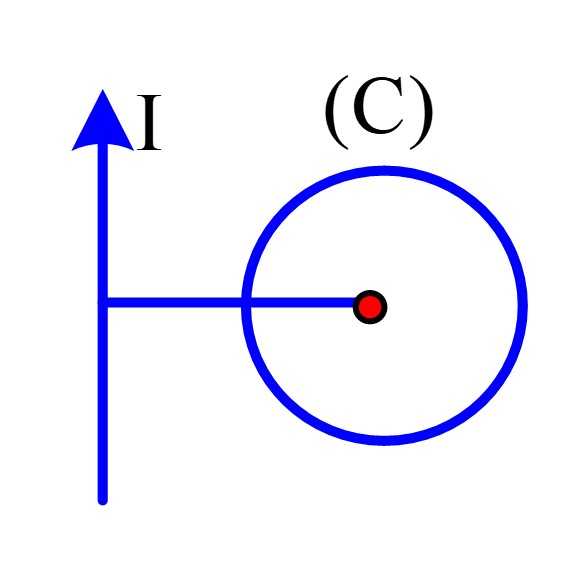
\includegraphics[scale=0.2]{../figs/VN11-PH-29-P-0191-1}
		\end{center}
		\begin{mcq}(1)
			\item{(C) dịch chuyển trong mặt phẳng P lại gần $I$ hoặc ra xa $I$.}
			\item{(C) dịch chuyển trong mặt phẳng P với vận tốc song song với dòng $I$.}
			\item{(C) cố định, dây dẫn thẳng mang dòng $I$ chuyển động tịnh tiến dọc theo chính nó.}
			\item{(C) quay xung quanh dòng điện thẳng $I$.}
		\end{mcq}
	}
	
	\loigiai{
		\textbf{Đáp án: A.}
		
		Vì từ trường của dòng điện thẳng I mạnh ở những điểm gần dòng điện và càng giảm ở những điểm càng xa dòng điện.
		
		Suy ra trường hợp (C) dịch chuyển trong P lại gần I hoặc ra xa I thì từ thông qua (C) biến thiên.
	}
	
	\item \mkstar{2} 
	
	\cauhoi{
	Cho một nam châm thẳng rơi theo phương thẳng đứng qua tâm $\text O$ của vòng dây dẫn tròn nằm ngang như hình vẽ. Trong quá trình nam châm rơi, vòng dây xuất hiện dòng điện cảm ứng có chiều
	\begin{center}
		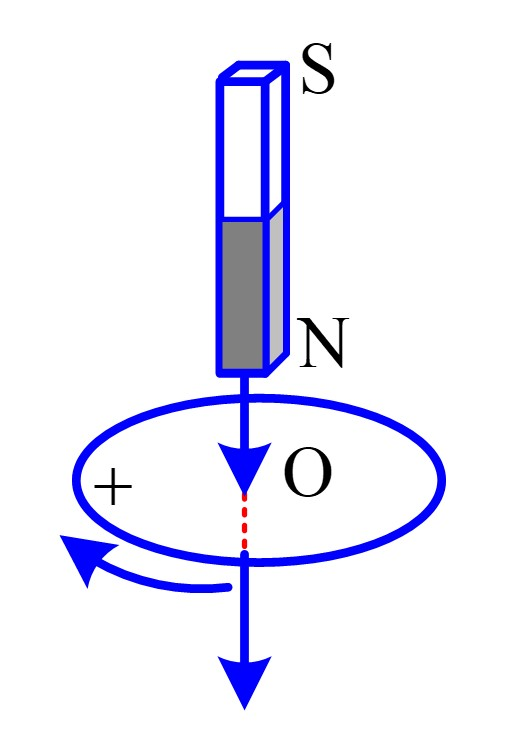
\includegraphics[scale=0.25]{../figs/VN11-PH-29-P-0191-2}
	\end{center}
	\begin{mcq}(1)
		\item là chiều dương quy ước trên hình.
		\item ngược với chiều dương quy ước trên hình.
		\item ngược với chiều dương quy ước khi nam châm ở phía trên vòng dây và chiều ngược lại khi nam châm ở phía dưới.
		\item là chiều dương quy ước khi nam châm ở phía trên vòng dây và chiều ngược lại khi nam châm ở phía dưới.
	\end{mcq}
		
	}
	
	\loigiai{
		\textbf{Đáp án: C.}
		

	}
	
	\item \mkstar{2} 
	
	\cauhoi{
		Chiều dòng điện cảm ứng trong vòng dây đúng là
		\begin{center}
			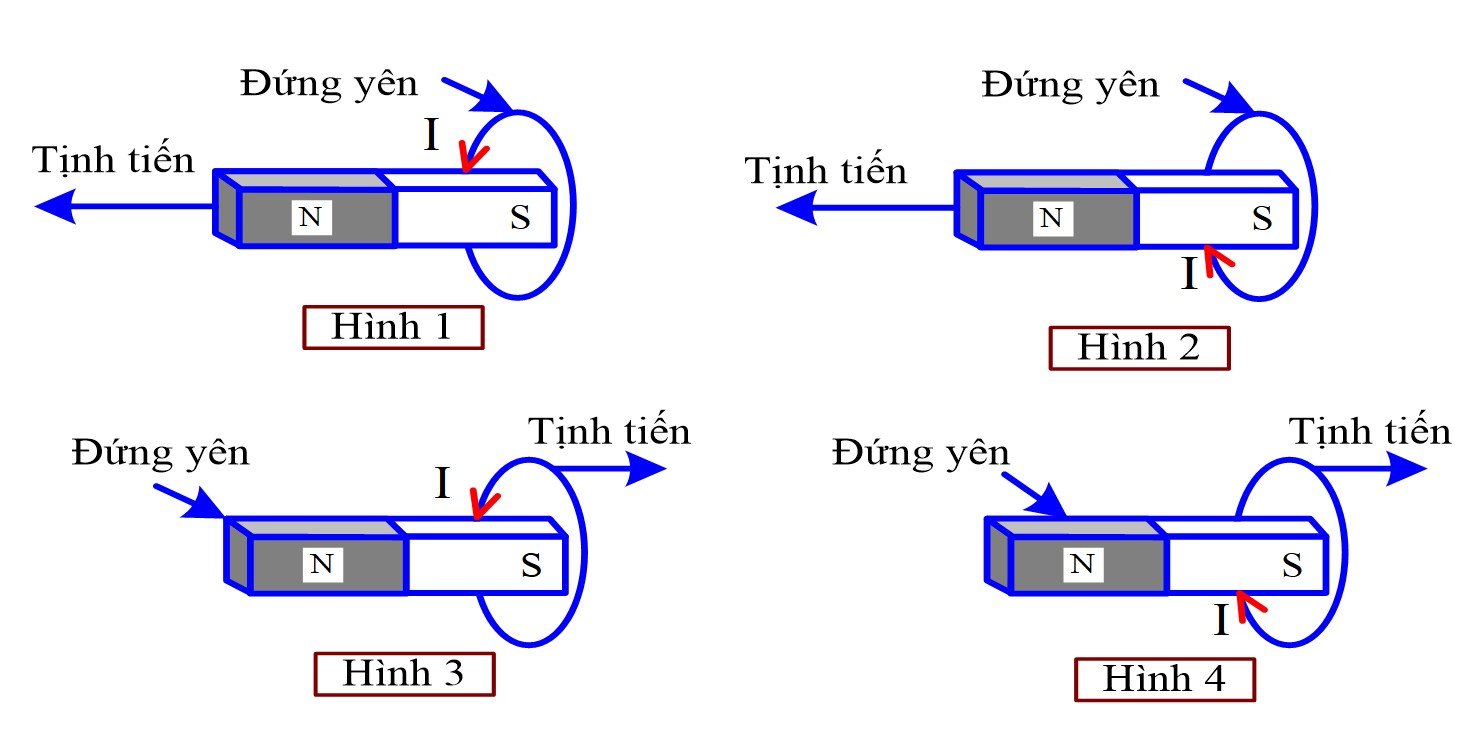
\includegraphics[scale=0.4]{../figs/VN11-PH-29-P-0191-3}
		\end{center}
		\begin{mcq}(2)
			\item{Hình 1 và Hình 2.}
			\item{Hình 1 và Hình 3.}
			\item{Hình 2 và Hình 4.}
			\item{Hình 4 và Hình 3.}
		\end{mcq}
	}
	
	\loigiai{
		\textbf{Đáp án: B.}
		
		
	}
	\item \mkstar{2} 
	
	\cauhoi{
		Một thanh nam châm NS được đặt thẳng đứng song song với mặt phẳng chứa vòng dây dẫn (C) và có trục quay O vuông góc với trục của vòng dây, chiều dương trên vòng dây được chọn như hình vẽ. Thanh nam châm NS chuyển động quay góc $\ang{90}$ để cực Nam (S) của nó tới đối diện với vòng dây dẫn (C) thì trong (C)
		\begin{center}
			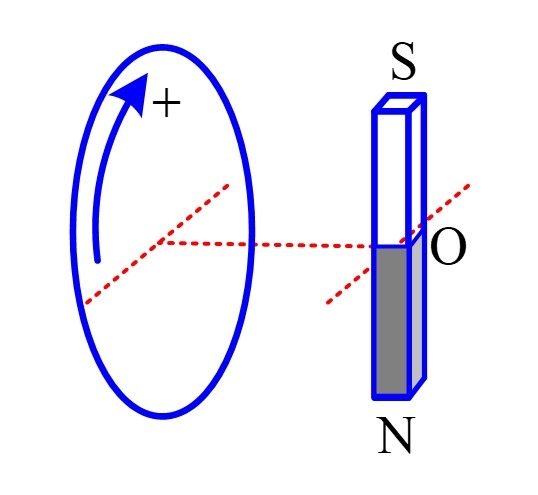
\includegraphics[scale=0.35]{../figs/VN11-PH-29-P-0191-4}
		\end{center}
		\begin{mcq}(1)
			\item{không có dòng điện cảm ứng.}
			\item{có dòng điện cảm ứng chạy theo chiều dương.}
			\item{có dòng điện cảm ứng chạy theo chiều âm.}
			\item{có dòng điện cảm ứng với cường độ biến thiên tuần hoàn theo thời gian.}
		\end{mcq}	
	}
	
	\loigiai{
		\textbf{Đáp án: C.}
		
		
	}
	\item \mkstar{2} 
	
	\cauhoi{
		Một khung dây dẫn tròn, nhẹ, được treo bằng sợi dây mềm, đường thẳng $x'x$ trùng với trục của khung dây, một nam châm thẳng đặt dọc theo trục $x'x$, cực Bắc của nam châm gần khung dây như hình vẽ. Tịnh tiến nam châm
		\begin{center}
			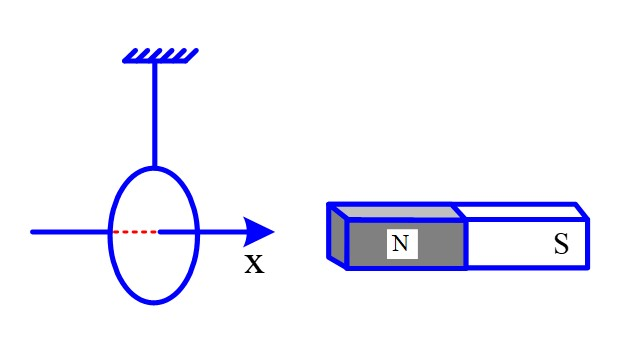
\includegraphics[scale=0.4]{../figs/VN11-PH-29-P-0191-5}
		\end{center}
		\begin{mcq}(1)
			\item{lại gần khung dây thì thấy khung dây chuyển động theo chiều dương trục $x'x$.}
			\item{lại gần khung dây thì thấy khung dây chuyển động theo chiều âm trục $x'x$.}
			\item{ra xa khung dây thì thấy khung dây chuyển động theo chiều âm trục $x'x$.}
			\item{thì chúng luôn đẩy khung dây.}
		\end{mcq}
	}
	
	\loigiai{
		\textbf{Đáp án: B.}
		
		
	}
	\item \mkstar{2} 
	
	\cauhoi{
		Một khung dây dẫn rất nhẹ được treo bằng sợi dây mềm, đường thẳng $x'x$ trùng với trục của khung dây. Khung dây được đặt gần một nam châm điện, trục nam châm điện trùng với trục $x'x$. Khi cho con chạy của biến trở dịch chuyển từ M đến N thì
		\begin{center}
			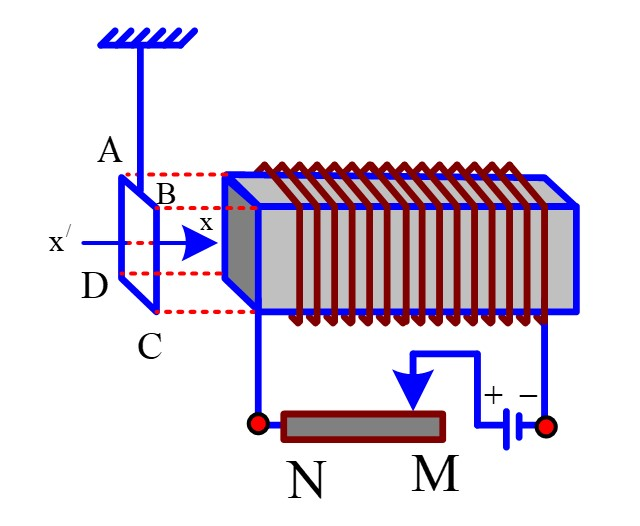
\includegraphics[scale=0.4]{../figs/VN11-PH-29-P-0191-6}
		\end{center}
		\begin{mcq}(1)
			\item{trong khung dây không có dòng điện cảm ứng.}
			\item{trong khung dây xuất hiện dòng điện cảm ứng có chiều ABCD.}
			\item{khung dây bị đẩy ra xa nam châm.}
			\item{khung dây bị hút lại gần nam châm.}
		\end{mcq}	
	}
	
	\loigiai{
		\textbf{Đáp án: C.}
		
		
	}
	\item \mkstar{2} 
	
	\cauhoi{
		Một khung dây dẫn tròn gồm $N$ vòng. Khung nằm trong từ trường đều, mặt phẳng khung song song với đường sức từ như hình vẽ. Cho khung quay xung quanh trục MN, qua tâm của khung và trùng với một đường sức từ thì
		\begin{center}
			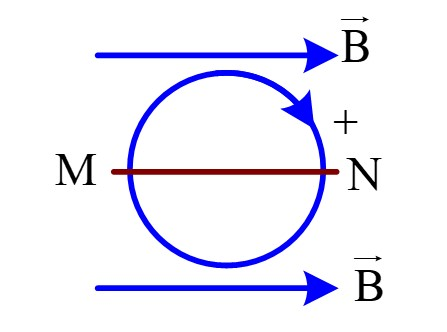
\includegraphics[scale=0.4]{../figs/VN11-PH-29-P-0191-7}
		\end{center}
		\begin{mcq}(1)
			\item{không có dòng điện cảm ứng.}
			\item{có dòng điện cảm ứng chạy theo chiều dương.}
			\item{có dòng điện cảm ứng chạy theo chiều âm.}
			\item{có dòng điện cảm ứng với cường độ biến thiên tuần hoàn theo thời gian.}
		\end{mcq}	
	}
	
	\loigiai{
		\textbf{Đáp án: A.}
		
		+ Lúc đầu vì B song song với mặt khung nên góc giữa B và pháp tuyến của khung là $90^\circ$ nên $\Phi = 0$
		
		+ Khi quay khung xung quanh trục MN như hình vẽ thì góc giữa B và pháp tuyến luôn là $90^\circ$.
		
		Suy ra không có dòng điện cảm ứng.
	}

		\item \mkstar{2} 
	
	\cauhoi{
		
		Cho dòng điện thẳng cường độ $I$ không đổi và khung dây dẫn hình chữ nhật MNPQ, cạnh MQ của khung sát với dòng điện như hình vẽ. Cho biết các dây dẫn đều có lớp vỏ cách điện. Cho khung dây dẫn quay xung quanh cạnh MQ của khung thì
		\begin{center}
			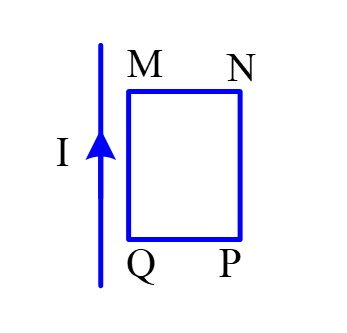
\includegraphics[scale=0.45]{../figs/VN11-PH-29-P-0191-8}
		\end{center}
		\begin{mcq}(1)
			\item{không có dòng điện cảm ứng.}
			\item{có dòng điện cảm ứng chạy theo chiều dương.}
			\item{có dòng điện cảm ứng chạy theo chiều âm.}
			\item{có dòng điện cảm ứng với cường độ biến thiên tuần hoàn theo thời gian.}
		\end{mcq}	
	}
	
	\loigiai{
		\textbf{Đáp án: A.}
		
		
	}
		\item \mkstar{2} 
	\cauhoi{
		
			Một vòng dây phẳng giới hạn diện tích $S=\SI{5}{\centi \meter \squared}$ đặt trong từ trường đều cảm ứng từ $B=\SI{0.1}{\tesla}$. Mặt phẳng vòng dây làm thành với từ trường một góc $\alpha = \ang{30}$. Tính từ thông qua $S$.
		\begin{mcq}(4)
			\item{$\SI{3e-4}{\weber}$.}
			\item{$\SI{3e-5}{\weber}$.}
			\item{$\SI{4.5e-5}{\weber}$.}
			\item{$\SI{2.5e-5}{\weber}$.}
		\end{mcq}	
	}
	
	\loigiai{
		\textbf{Đáp án: D.}
		
		Mặt phẳng vòng dây làm thành với B một góc $30^\circ$ nên $\alpha  = 60^\circ.$
		
		Từ thông qua $S$
		
		$$\Phi = BS \cos \alpha  = \SI{2.5e-5}{\weber}.$$
	}
		\item \mkstar{2} 
	\cauhoi{
		
		Một khung dây hình tròn đặt trong từ trường đều có cảm ứng từ $B=\SI{0.06}{\tesla}$ sao cho mặt phẳng khung dây vuông góc với các đường sức từ. Từ thông qua khung dây là $\SI{1.2e-5}{\weber}$. Bán kính vòng dây gần giá trị nào nhất sau đây?
		\begin{mcq}(4)
			\item{$\SI{12}{\milli \meter}$.}
			\item{$\SI{6}{\milli \meter}$.}
			\item{$\SI{7}{\milli \meter}$.}
			\item{$\SI{8}{\milli \meter}$.}
		\end{mcq}	
	}
	
	\loigiai{
		\textbf{Đáp án: D.}
		
		Bán kính vòng dây
		
		$$ R = \sqrt {\dfrac{\phi}{B \pi \cos \alpha}} = 8 \cdot 10^{-3}\ \text{m}.$$
	}
		\item \mkstar{2} 
	\cauhoi{
		
			Một khung dây phẳng giới hạn diện tích $S=\SI{5}{\centi \meter \squared}$ gồm 20 vòng dây đặt trong từ trường đều có cảm ứng từ $B=\SI{0.1}{\tesla}$ sao cho mặt phẳng khung dây hợp với vectơ cảm ứng từ một góc $\ang{60}$. Tính từ thông qua diện tích giới hạn bởi khung dây.
		\begin{mcq}(4)
			\item{$\SI{8.66e-4}{\weber}$.}
			\item{$\SI{5e-4}{\weber}$.}
			\item{$\SI{4.5e-5}{\weber}$.}
			\item{$\SI{2.5e-5}{\weber}$.}
		\end{mcq}	
	}
	
	\loigiai{
		\textbf{Đáp án: A.}
		
		Góc hợp bởi giữa pháp tuyển và cảm ứng từ $\alpha  = 30^\circ.$
		
		Từ thông qua diện tích $S$
		
		$$\Phi = NBS \cos \alpha  = \text{8,66} \cdot 10^{-4}\ \text{Wb}.$$
	}
		\item \mkstar{2} 
	\cauhoi{
		
		Một khung dây hình vuông cạnh $\SI{5}{\centi \meter}$ đặt trong từ trường đều có cảm ứng từ $B=\SI{8e-4}{\tesla}$. Từ thông qua hình vuông đó bằng $\SI{e-6}{\weber}$. Tính góc hợp giữa vectơ cảm ứng từ và vectơ pháp tuyến của hình vuông đó.
		\begin{mcq}(4)
			\item{$\alpha = \ang{0}$.}
			\item{$\alpha=\ang{30}$.}
			\item{$\alpha=\ang{60}$.}
			\item{$\alpha=\ang{90}$.}
		\end{mcq}	
	}
	
	\loigiai{
		\textbf{Đáp án: B.}
		
		Diện tích của khung
		
		$$S = a^2 = \text{2,5} \cdot 10^{-3}\ \text{m}^2.$$
		
		Góc hợp giữa vectơ cảm ứng từ và vectơ pháp tuyến 
		
		$$ \Phi = BS \cos \alpha \Rightarrow \alpha  = 60^\circ.$$
	}
		\item \mkstar{2} 
	\cauhoi{
		
		[Đề tham khảo của BGD-ĐT-2018] Một khung dây phẳng diện tích $\SI{20}{\centi \meter \squared}$ đặt trong từ trường đều có vectơ cảm ứng từ hợp với vectơ pháp tuyến của mặt phẳng khung dây một góc $\ang{60}$ và có độ lớn $\SI{0.12}{\tesla}$. Từ thông qua khung dây này là
		\begin{mcq}(4)
			\item{$\SI{2.4e-4}{\weber}$.}
			\item{$\SI{1.2e-4}{\weber}$.}
			\item{$\SI{1.2e-6}{\weber}$.}
			\item{$\SI{2.4e-6}{\weber}$.}
		\end{mcq}	
	}
	
	\loigiai{
		\textbf{Đáp án: B.}
		
		Từ thông qua khung dây:
		
		$$\Phi  = BS\cos \alpha  = \text{1,2} \cdot 10^{-4} \ \text{Wb}.$$
	}

\end{enumerate}
\section{Suất điện động cảm ứng}
\begin{enumerate}[label=\bfseries Câu \arabic*:]
	
	\item \mkstar{2} 
	
	\cauhoi{
		Cuộn dây có $N=100$ vòng, mỗi vòng có diện tích $S=\SI{300}{\centi \meter \squared}$, đặt trong từ trường đều có cảm ừng từ $B=\SI{0.2}{\tesla}$ sao cho trục của cuộn dây song song với các đường sức từ. Quay đều cuộn dây để sau $\Delta t= \SI{0.5}{\second}$ trục của nó vuông góc với các đường sức từ thì độ lớn suất điện động cảm ứng trung bình trong cuộn dây là
		\begin{mcq}(4)
			\item{$\SI{0.6}{\volt}$.}
			\item{$\SI{1.2}{\volt}$.}
			\item{$\SI{3.6}{\volt}$.}
			\item{$\SI{4.8}{\volt}$.}
		\end{mcq}
	}
	
	\loigiai{
		
		\textbf{Đáp án: B.}
		
		Suất điện động cảm ứng
		
		$$e_\text{c} = \left|\dfrac{\Delta \Phi}{\Delta t} \right| = \left|\dfrac{NBS (\cos \alpha_2 - \cos \alpha_1)}{\Delta t} \right| = \SI{1,2}{V}.$$
		
		
	}
	
	\item \mkstar{2}
	
	\cauhoi{
	Một khung dây có $100$ vòng được đặt trong từ trường đều sao cho các đường sức từ vuông góc với mặt phẳng của khung dây. Diện tích của mỗi vòng dây là $\SI{2}{\deci \meter \squared}$, cảm ứng từ giảm đều từ $\SI{0.5}{\tesla}$ đến $\SI{0.2}{\tesla}$ trong thời gian $\SI{0.1}{\second}$. Suất điện động cảm ứng trong khung dây là
	\begin{mcq}(4)
		\item{$\SI{6}{\volt}$.}
		\item{$\SI{60}{\volt}$.}
		\item{$\SI{3}{\volt}$.}
		\item{$\SI{30}{\volt}$.}
	\end{mcq}
	}
	\loigiai{
		
		\textbf{Đáp án: A.}
		
		Suất điện động cảm ứng trong khung dây
		
		$$e_\text c = \dfrac{\Delta \Phi}{\Delta t} = \dfrac{N \Delta B S \cos \alpha}{\Delta t} = \SI{6}{V}.$$
	}

	\item \mkstar{2} 
	
	\cauhoi{
		Một khung dây hình vuông có cạnh $\SI{5}{\centi \meter}$, đặt trong từ trường đều $\SI{0.08}{\tesla}$, mặt phẳng khung dây vuông góc với các đường sức từ. Trong thời gian $\SI{0.2}{\second}$, cảm ứng từ giảm xuống đến $0$. Độ lớn của suất điện động cảm ứng trong khung trong khoảng thời gian đó là
		\begin{mcq}(4)
			\item{$\SI{0.04}{\milli \volt}$.}
			\item{$\SI{0.5}{\milli \volt}$.}
			\item{$\SI{1}{\milli \volt}$.}
			\item{$\SI{8}{\volt}$.}
		\end{mcq}
	}
	
	\loigiai{
		\textbf{Đáp án: C.}
		
		Suất điện động cảm ứng
	
	$$e_\text{c} = \left|\dfrac{\Delta \Phi}{\Delta t} \right| = \left|\dfrac{BS \cos \alpha}{\Delta t} \right| = \SI{1}{mV}.$$
	}

		\item \mkstar{2} 
	
	\cauhoi{
		[Đề chính thức của BGD-ĐT-2018] Một vòng dây kín, phẳng được đặt trong từ trường đều. Trong khoảng thời gian $\SI{0.02}{\second}$, từ thông qua vòng dây giảm đều từ giá trị $\SI{4e-3}{\weber}$ về $0$ thì suất điện động cảm ứng xuất hiện trong vòng dây có độ lớn
		\begin{mcq}(4)
			\item{$\SI{0.2}{\volt}$.}
			\item{$\SI{8}{\volt}$.}
			\item{$\SI{2}{\volt}$.}
			\item{$\SI{0.8}{\volt}$.}
		\end{mcq}
		
	}
	\loigiai{
		
		\textbf{Đáp án: A.}
		
			Suất điện động cảm ứng
		
		$$e_\text{c} = \left|\dfrac{\Delta \Phi}{\Delta t} \right|  = \SI{0,2}{V}.$$
	}
		\item \mkstar{2} 
	
	\cauhoi{
		Thanh kim loại AB dài $\SI{20}{\centi \meter}$ kéo trượt đều trên hai thanh ray kim loại nằm ngang như hình vẽ.
		\begin{center}
			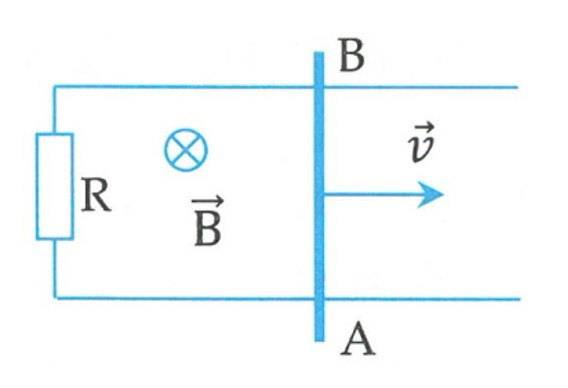
\includegraphics[scale=0.4]{../figs/VN11-PH-30-P-0201-1.jpg}
		\end{center}
		Các dây nối nhau bằng điện trở $R=\SI{3}{\Omega}$. Vận tốc của thanh AB là $\SI{12}{\meter / \second}$. Hệ thống đặt trong từ trường đều có $B=\SI{0.4}{\tesla}$, $\vec{B}$ vuông góc với mạch điện. Tìm suất điện động cảm ứng trong khung.
			\begin{mcq}(4)
				\item{$\SI{0.48}{\volt}$.}
				\item{$\SI{0.96}{\volt}$.}
				\item{$\SI{0.83}{\volt}$.}
				\item{$\SI{0.69}{\volt}$.}
			\end{mcq}
		
	}
	\loigiai{
		
		\textbf{Đáp án: B.}
		
		Suất điện động cảm ứng trong thanh
		
		$$e_\text c = Bvl \sin 90^\circ = \SI{0,96}{V}.$$ 
	}
	
	
\end{enumerate}

\section{Tự cảm}
\begin{enumerate}[label=\bfseries Câu \arabic*:]
	
	\item \mkstar{2} 
	
	\cauhoi{
		Ống dây điện hình trụ có chiều dài tăng gấp đôi (các đại lượng khác không thay đổi) thì độ tự cảm
	\begin{mcq}(2)
		\item {không đổi.}
		\item {tăng 4 lần.}
		\item {tăng 2 lần.}
		\item {giảm 2 lần.}
	\end{mcq}
	}
	
	\loigiai{
		\textbf{Đáp án: D.}
		
	Độ tự cảm của ống dây 
	
	$$ L =4\pi 10^{-7} \dfrac{N^2}{l}S.$$
	}
	
	\item \mkstar{2} 
	
	\cauhoi{
		Ống dây điện hình trụ có số vòng dây tăng 2 lần (các đại lượng khác không thay đổi) thì độ tự cảm
		\begin{mcq}(2)
			\item{tăng 2 lần.}
			\item{tăng 4 lần.}
			\item{giảm 2 lần.}
			\item{giảm 4 lần.}
		\end{mcq}
		
	}
	\loigiai{
		
		\textbf{Đáp án: B.}
		
		Độ tự cảm của ống dây 
	
	$$ L =4\pi 10^{-7} \dfrac{N^2}{l}S.$$
	}
	
	\item \mkstar{2}
	
	\cauhoi{
		Ống dây điện hình trụ có số vòng dây tăng 4 lần và chiều dài tăng 2 lần (các đại lượng khác không thay đổi) thì độ tự cảm
		\begin{mcq}(2)
			\item{tăng 8 lần.}
			\item{tăng 4 lần.}
			\item{giảm 2 lần.}
			\item{giảm 4 lần.}
		\end{mcq}
		
	}
	\loigiai{
		
		\textbf{Đáp án: A.}
	
	Độ tự cảm của ống dây 
	
	$$ L =4\pi 10^{-7} \dfrac{N^2}{l}S.$$
	}

		\item \mkstar{2} 
	
	\cauhoi{
	Tính độ tự cảm của một ống dây hình trụ có chiều dài $\SI{0.5}{\meter}$ gồm $1000$ vòng dây, mỗi vòng dây có đường kính $\SI{20}{\centi \meter}$.
	\begin{mcq}(4)
		\item{$\SI{0.088}{\henry}$.}
		\item{$\SI{0.079}{\henry}$.}
		\item{$\SI{0.125}{\henry}$.}
		\item{$\SI{0.064}{\henry}$.}
	\end{mcq}	
		
	}
	\loigiai{
		
		\textbf{Đáp án: B.}
	
	Độ tự cảm của ống dây 
	
	$$ L =4\pi 10^{-7} \dfrac{N^2}{l}S=\SI{0.079}{\henry}.$$
	}
	
		\item \mkstar{2} 
	
	\cauhoi{
		[Đề chính thức của BGD-ĐT-2018] Một cuộn cảm có độ tự cảm $\SI{0.2}{\henry}$. Trong khoảng thời gian $\SI{0.05}{\second}$, dòng điện trong cuộn cảm có cường độ giảm đều từ $\SI{2}{\ampere}$ xuống $0$ thì suất điện động tự cảm xuất hiện trong cuộn cảm có độ lớn là
		\begin{mcq}(4)
			\item{$\SI{4}{\volt}$.}
			\item{$\SI{0.4}{\volt}$.}
			\item{$\SI{0.02}{\volt}$.}
			\item{$\SI{8}{\volt}$.}
		\end{mcq}
		
	}
	\loigiai{
		
		\textbf{Đáp án: D.}
		
		Suất điện động tự cảm
		
		$$|e_\text{tc} |= L \dfrac{|\Delta i|}{\Delta t} = \SI{8}{V}.$$
	}
	
		\item \mkstar{2} 
	
	\cauhoi{
		Một cuộn cảm có độ tự cảm $\SI{0.5}{\henry}$, trong đó dòng điện tăng đều với tốc độ $\SI{200}{\ampere / \second}$ thì suất điện động tự cảm là
		\begin{mcq}(4)
			\item{$\SI{-100}{\volt}$.}
			\item{$\SI{20}{\volt}$.}
			\item{$\SI{100}{\volt}$.}
			\item{$\SI{200}{\volt}$.}
		\end{mcq}
		
	}
	\loigiai{
		
		\textbf{Đáp án: A.}
		
			Suất điện động tự cảm
		
		$$e_\text{tc} = - L \dfrac{\Delta i}{\Delta t} = -\SI{100}{V}.$$
	}
	
		\item \mkstar{2} 
	
	\cauhoi{
			Dòng điện qua một ống dây không có lõi sắt biến đổi theo thời gian. Trong thời gian $\SI{0.01}{\second}$ cường độ dòng điện tăng từ $i_1=\SI{1}{\ampere}$ đến $i_2=\SI{2}{\ampere}$, suất điện động tự cảm trong ống dây có độ lớn bằng $\SI{20}{\volt}$. Hệ số tự cảm của ống dây là
		\begin{mcq}(4)
			\item{$\SI{0.1}{\henry}$.}
			\item{$\SI{0.4}{\henry}$.}
			\item{$\SI{0.2}{\henry}$.}
			\item{$\SI{0.6}{\henry}$.}
		\end{mcq}
		
	}
	\loigiai{
		
		\textbf{Đáp án: C.}
		
		
		Hệ số tự cảm của ống dây
		
		$$ L  = \dfrac{|e_\text{tc}|\Delta t}{|\Delta i|} =\SI{0,2}{H}.$$
	}
	
		\item \mkstar{2}
	
	\cauhoi{
	Suất điện động tự cảm $\SI{0.75}{\volt}$ xuất hiện trong một cuộn cảm có $L=\SI{25}{\milli \henry}$, tại đó cường độ dòng điện giảm từ giá trị $I$ xuống $0$ trong $\SI{0.01}{\second}$. Tính $I$.
	\begin{mcq}(4)
		\item{$\SI{0.1}{\ampere}$.}
		\item{$\SI{0.4}{\ampere}$.}
		\item{$\SI{0.3}{\ampere}$.}
		\item{$\SI{0.6}{\ampere}$.}
	\end{mcq}
		
	}
	\loigiai{
		
		\textbf{Đáp án: C.}
		
		Cường độ dòng điện
		
		$$I = \dfrac{|e_\text{tc}| \Delta t}{L} = \SI{0,3}{A}.$$ 
	}
	
		\item \mkstar{2}
	
	\cauhoi{
			Trong một mạch kín có độ tự cảm $\SI{0.5e-3}{\henry}$, nếu suất điện động tự cảm có độ lớn bằng $\SI{0.25}{\volt}$ thì tốc độ biến thiên của dòng điện là
		\begin{mcq}(4)
			\item{$\SI{250}{\ampere / \second}$.}
			\item{$\SI{400}{\ampere / \second}$.}
			\item{$\SI{600}{\ampere / \second}$.}
			\item{$\SI{500}{\ampere / \second}$.}
		\end{mcq}
		
	}
	\loigiai{
		
		\textbf{Đáp án: D.}
		
		Tốc độ biến thiên của dòng điện
		
		$$\left|\dfrac{\Delta i}{\Delta r}\right| = \dfrac{|e_\text{tc}|}{L} = \SI{500}{\ampere / \second}.$$
	}
	
		\item \mkstar{2} 
	
	\cauhoi{
			Một ống dây dài $l=\SI{30}{\centi \meter}$ gồm $N=1000$ vòng dây, đường kính mỗi vòng dây $d=\SI{8}{\centi \meter}$ có dòng điện với cường độ $i=\SI{2}{\ampere}$ đi qua. Tính từ thông qua mỗi vòng dây
		\begin{mcq}(4)
			\item{$\SI{42}{\micro \weber}$.}
			\item{$\SI{0.4}{\micro \weber}$.}
			\item{$\SI{0.2}{\micro \weber}$.}
			\item{$\SI{86}{\micro \weber}$.}
		\end{mcq}
		
	}
	\loigiai{
		
		\textbf{Đáp án: B.}
		
		Từ thông qua ống dây
		
		$$ \Phi = L i = 4 \pi 10^{-7} \dfrac{N^2}{l} S i =\SI{0,04}{Wb}.$$
		
		Từ thông qua mỗi vòng dây
		
		$$ \phi = \dfrac{\Phi}{N} = 4 \cdot 10^{-5}\ \text{Wb}.$$
	}
	
		\item \mkstar{2} 
	
	\cauhoi{
		Một ống dây dài $l=\SI{30}{\centi \meter}$ gồm $N=1000$ vòng dây, đường kính mỗi vòng dây $d=\SI{8}{\centi \meter}$ có dòng điện với cường độ $i=\SI{2}{\ampere}$ đi qua. Thời gian ngắt dòng điện là $t=\SI{0.1}{\second}$, độ lớn suất điện động tự cảm xuất hiện trong ống dây là
		\begin{mcq}(4)
			\item{$\SI{0.15}{\volt}$.}
			\item{$\SI{0.42}{\volt}$.}
			\item{$\SI{0.24}{\volt}$.}
			\item{$\SI{8.6}{\volt}$.}
		\end{mcq}
		
	}
	\loigiai{
		
		\textbf{Đáp án: B.}
		
		Suất điện động tự cảm
		
		$$|e_\text{tc} |=  \left|- 4 \pi 10^{-7} \dfrac{N^2}{l} S \dfrac{\Delta i}{\Delta t}\right| = \SI{0,42}{V}.$$
	}
	
\end{enumerate}	
\whiteBGstarEnd
	\stopcontents[mychapters]
	
\setcounter{mychapter}{25}
	\mychapter{Khúc xạ ánh sáng}
	\startcontents[mychapters]
	\printcontents[mychapters]{}{0}{\setcounter{tocdepth}{1}}
	\whiteBGstarBegin
\setcounter{section}{0}
\section{Lý thuyết: Khúc xạ ánh sáng. Chiết suất của môi trường}
\begin{enumerate}[label=\bfseries Câu \arabic*:]
	
		\item \mkstar{1} [21]
	
	\cauhoi{
		
		Chiết suất tuyệt đối của một môi trường truyền ánh sáng
		
		
		\begin{mcq}(2)
			\item luôn lớn hơn 1.
			\item luôn nhỏ hơn 1.	
			\item luôn lớn hơn 0.
			\item luôn bằng 1.
		\end{mcq}
	}
	
	\loigiai{
		
		\textbf{Đáp án: A.}
		
		Chiết suất của chân không đối với ánh sáng là 1. Chiết suất tuyệt đối của một môi trường truyền ánh sáng rắn, lỏng, khí bất kì đều lớn hơn trong chân không.
		
		
		
	}
	

	\item \mkstar{1} [21]
	
	\cauhoi{
		
		Khi ánh sáng truyền từ môi trường có chiết suất $n_1$ sang môi trường có chiết suất $n_2$. Gọi $i$ và $r$ lần lượt là góc tới và góc khúc xạ. Định luật khúc xạ ánh sáng được viết theo hệ thức:
		
		\begin{mcq}(2)
			\item $n_2 \sin i = n_1 \sin r.$
			\item $\dfrac{\sin i}{\sin r} = \dfrac{n_1}{n_2}.$
			\item $\dfrac{\sin i}{\sin r} = \dfrac{n_2}{n_1}.$
			\item $\dfrac{r}{i} = \dfrac{n_2}{n_1}.$
		\end{mcq}
	}
	
	\loigiai{
		
	\textbf{Đáp án: C.}
		
		Khi $n_{21} > 1 (r < i)$  hoặc khi môi trường (2) chiết quang hơn môi trường (1)
		
		
		
	}
	
		\item \mkstar{1} [18]
	
	\cauhoi{
		Khi nào tia khúc xạ bị lệch về gần pháp tuyến hơn so với hướng của tia tới?
		
	}
	
	\loigiai{
		
	Khi $n_{21} > 1 (r < i)$  hoặc khi môi trường (2) chiết quang hơn môi trường (1)
	
		
		
	}

		\item \mkstar{1} [19]
	
	\cauhoi{
		
	Chiết suất tuyệt đối của một môi trường là gì ?
	
		
	}
	
	\loigiai{
		
		Chiết suất tuyệt đối của một môi trường là tỉ số vận tốc ánh sáng $c$ trong chân không so với vận tốc ánh sáng $v$ trong môi trường đó.
		
		$$n =\dfrac{c}{v}.$$
		
		Hệ thức liên hệ giữa chiết suất tỉ đối và chiết suất tuyệt đối
		
		$$n_{21} = \dfrac{n_2}{n_1}.$$
		
		
		
	}
	\item \mkstar{1} [12]
	
	\cauhoi{
		Tại sao vào mùa nắng, lúc trưa nắng trên đường nhựa khô ráo, nhìn từ xa ta lại thấy mặt đường nhựa như có nước làm ướt?
		\begin{center}
			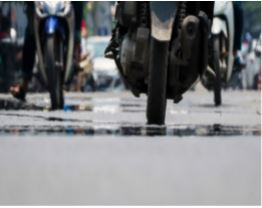
\includegraphics[scale=0.9]{../figs//VN11-2021-PH-TP028-05.JPG}
		\end{center}
	}
	
	\loigiai{
		
		- Đường nhựa có màu đen nên nên hấp thụ ánh sáng Mặt Trời mạnh và trở nên rất nóng. Lượng nhiệt này sau đó bức xạ trở lại làm nóng lớp không khí ở sát mặt đường khiến chiết suất giảm đi.
		
		- Tia sáng từ 1 vật thể ở xa như ô tô, xe máy.... bị khúc xạ nhiều lần qua những lớp không khí có chiết suất khác nhau và có xu hướng bẻ cong thoai thoải xuống mặt đường. Và tại đây ánh sáng bị phản xạ toàn phần tại mặt phân cách giữa lớp không khí lạnh (có chiết suất cao) và lớp không khí nóng (có chiết suất thấp) đến mắt ta khiến ta thấy bóng lờ mờ của vật thể phía trước thấp thoáng trên mặt đường. Cùng với hiện tượng đối lưu không khí nên ta cảm nhận thấy như có vũng nước trước mặt
		
		
	}
	
	\item \mkstar{1} [36]
	
	\cauhoi{
		Sử dụng nội dung kiến thức đã học ở chương Khúc xạ ánh sáng trả lời các câu hỏi sau:
		\begin{enumerate}[label=\alph*)]
			\item 	Hiện tượng khúc xạ ánh sáng là gì? 
			\item	Hãy phát biểu nội dung của định luật khúc xạ ánh sáng?
			\item   Nêu công thức liên hệ giữa chiết suất và góc tới, góc khúc xạ? 
		\end{enumerate}
		
	}
	\loigiai{

		\begin{enumerate}[label=\alph*)]
			\item Hiện tượng khúc xạ ánh sáng là hiện tượng lệch phương của các tia sáng khi truyền xiên góc qua mặt phân cách giữa 2 môi trường trong suốt khác nhau.
			\item Định luật khúc xạ ánh sáng.
			
			+ Tia sáng nằm trong mặt phẳng tới và ở phía bên kia pháp tuyến so với tía tới.
			
			+ Với hai môi trường trong suốt nhất định, tỉ số giữa sin góc tới ($\sin i$) và sin góc khúc xạ ($\sin r$) luôn không đổi.
			\item 
			    Công thức liên hệ giữa chiết suất và góc tới, góc khúc xạ:
			    
			    $$n_1 \sin i = n_2 \sin r.$$
			    
			    Trong đó:	
			    
			    + $n_1, n_2$ là chiết suất của môi trường 1, 2
			    
			    + $i$ là góc tới
			    
			    + $r$ là góc khúc xạ    
		\end{enumerate}
	}
	\item \mkstar{1} [6]
	
	\cauhoi{
		Thế nào là hiện tượng khúc xạ ánh sáng? Phát biểu định luật khúc xạ ánh sáng.
	}
	
	\loigiai{
		
		
		Khúc xạ ánh sáng là hiện tượng lệch phương (gãy) của các tia sáng khi truyền xiên góc qua mặt phân cách giữa hai môi trường trong suốt khác nhau. 
		
		Định luật khúc xạ ánh sáng:
		
		- Tia khúc xạ nằm trong mặt phẳng tới (tạo bởi tia tới và pháp tuyến) và ở phía bên kia pháp tuyến so với tia tới. 
		
		- Với hai môi trường trong suốt nhất định, tỉ số giữa sin góc tới ($\sin i$) và sin góc khúc xạ ($\sin r$) luôn luôn không đổi: 
		
		$$\dfrac{\sin i}{\sin r} =\text{hằng số}.$$
		
	}
	
	
	\item \mkstar{2} [9]
	
	\cauhoi{
		
		Chúng tôi xin chia sẻ bài viết của nhiếp ảnh gia Simon Bond từ Digital Photography School cho những ai có đam mê nhiếp ảnh, muốn chụp được những bức ảnh ấn tượng với quả cầu pha lê.
		
		Có thể em đã nghe về sự phản xạ trong nhiếp ảnh, nhưng có bao giờ em thử sức với ảnh khúc xạ chưa? Nếu sử dụng đúng cách, khúc xạ sẽ tạo ra những hình ảnh hấp dẫn khiến người xem ấn tượng mạnh và vô cùng tò mò. 
		
		(Nguồn: \textit{https://viettimes.vn/7-bi-quyet-chup-anh-khuc-xa-voi-qua-cau-pha-le-90224.html})
		\begin{enumerate}[label=\alph*)]
			\item Dựa vào kiến thức đã học, em hãy cho biết thế nào là khúc xạ ánh sáng? 
			\item Nêu định luật khúc xạ ánh sáng? Từ định luật hãy nhận định phát biểu sau đúng hay sai?
			
			+ Phát biểu 1: “Khi góc tới tăng dần thì góc khúc xạ cũng tăng dần”.
			
			+ Phát biểu 2: “Góc khúc xạ tỉ lệ thuận với góc tới”.
		\end{enumerate}

		\begin{center}
			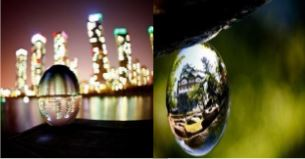
\includegraphics[scale=0.9]{../figs//VN11-2021-PH-TP028-02.JPG}
		\end{center}
	}
	
	\loigiai{
		
		\begin{enumerate}[label=\alph*)]
			\item Hiện tượng khúc xạ ánh sáng là hiện tượng lệch phương (gãy) của các tia sáng khi truyền xiên góc qua mặt phân cách giữa hai môi trường trong suốt khác nhau. 
			\item - Tia khúc xạ nằm trong mặt phẳng tới (tạo bởi tia tới và pháp tuyến), ở phía bên kia pháp tuyến so với tia tới.
										
				- Với hai môi trường trong suốt nhất định, tỉ số giữa sin góc tới và sin góc khúc xạ luôn không đổi.
				
				- Phát biểu 1: đúng								
	
				- Phát biểu 2 sai.	
	
		\end{enumerate}
	}

	
\end{enumerate}
\section{Dạng bài: Khúc xạ ánh sáng. Chiết suất của môi trường}
\begin{enumerate}[label=\bfseries Câu \arabic*:]
		\item \mkstar{2} [25]
	
	\cauhoi{
		
		Một tia sáng đi từ một chất lỏng có chiết suất $n = \sqrt 2$ ra không khí dưới góc tới $i = 30^\circ$. Vẽ đường đi của tia sáng. Tính góc khúc xạ $r$.
		
	}
	
	\loigiai{
	
	Ta có:
	
	$$n \sin i = \sin r \Rightarrow r = 45^\circ.$$
		
	}
	\item \mkstar{2} [22]
	
	\cauhoi{
		Một tia sáng truyền từ môi trường trong suốt có chiết suất $n$ ra không khí, dưới góc tới $30^\circ$ thì tia khúc xạ ra không khí lệch so với tia tới một góc bằng $15^\circ$. Xác định giá trị chiết suất $n$ của môi trường.
		
		
	}
	\loigiai{
		
		
		Chiết suất $n$ của môi trường
		
		$$D = r - i  \Rightarrow r = 45^\circ.$$ 
		
		$$n\sin i = \sin r$$        
		
		$$\Rightarrow n = \sqrt 2.$$
		
	}
	
	\item \mkstar{2} [18]
	\cauhoi{
		
	Tia sáng đơn sắc truyền từ không khí  vào khối thủy tinh có chiết suất 1,73. Tia khúc xạ và tia phản xạ ở mặt phân cách vuông góc với nhau. Tính góc tới của tia sáng và góc lệch giữa tia tới và tia ló.
	
		
	}
	\loigiai{
		
		Góc tới của tia sáng
		  
		$$r= 90^\circ - i.$$
		 
		$$\sin i = n \sin r$$
		 
		$$\tan i = n  \Rightarrow   i = 60^\circ$$
		
		Góc lệch giữa tia tới và tia khúc xạ 
		
		$$D= i-r =30^\circ$$
		
		
	}
	
	
	\item \mkstar{2} [7]
	
	\cauhoi{
		
		Một tia sáng đi từ không khí vào nước biển với góc tới $30^\circ$. Chiết suất của nước biển là $\dfrac{4}{3}$ và của không khí là $1$.
		
		\begin{enumerate}[label=\alph*)]
			\item Tính góc khúc xạ trong nước biển.
			\item Một người thợ lặn lặn sâu $\SI{5}{m}$ dưới mực nước biển khi ngước nhìn lên mặt biển sẽ trông thấy có một vùng sáng ngay trên đỉnh đầu. Vùng sáng có hình dạng gì? Kích thước như thế nào?
		\end{enumerate}
		
	}
	
	\loigiai{
		
		\begin{center}
			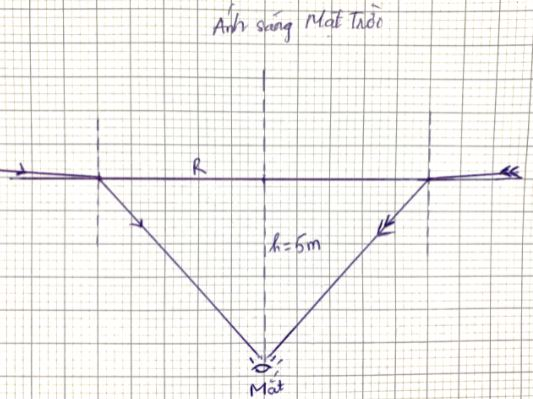
\includegraphics[scale=0.9]{../figs//VN11-2021-PH-TP028-01.JPG}
		\end{center}
		
		\begin{enumerate}[label=\alph*)]
			\item Góc khúc xạ trong nước biển 
			
			$$ n_1 \sin i = n_2 \sin r \Rightarrow r \approx 22^\circ.$$
			
			\item Vùng sáng là hình tròn.
			
			$$n_1 \sin i  = n_2 \sin r \Rightarrow r_\text{max} = \text{48,6}^\circ.$$
			
			Ta có: 
			
			$$\tan \text{48,6}^\circ =\dfrac{R}{h}.$$
			
			Suy ra: $R = \SI{5,67}{m}$.
			
			Hình tròn có bán kính $\SI{5,67}{m}$.
			
		\end{enumerate}
		
	}

			\item \mkstar{2} [14]
	
	\cauhoi{
		Chiếu một tia sáng từ không khí vào thủy tinh có chiết suất $\sqrt 2$  với góc tới $60^\circ$. Hãy tính góc khúc xạ và vẽ hình trong trường hợp đó.
		
	}
	
	\loigiai{
		
		Áp dụng định luật khúc xạ ta có:
		
		$$n_1\sin i = n_2 \sin r \Rightarrow r \approx 37^\circ45'.$$
	}
	
	\item \mkstar{2} [9]
	
	\cauhoi{
		
		Một tia sáng chiếu từ không khí đến một môi trường có chiết suất $\sqrt 2$ dưới góc tới $45^\circ$. 
		\begin{enumerate}[label=\alph*)]
			\item Tính góc khúc xạ của tia sáng.
			\item Tính góc lệch giữa tia tới và tia khúc xạ.
			\item Vẽ hình.
		\end{enumerate}
		
	}
	
	\loigiai{
		
		\begin{enumerate}[label=\alph*)]
			\item Góc khúc xạ của tia sáng
			
			$$n_1\sin i = n_2 \sin r \Rightarrow r = 30^\circ.$$ 
			
			
			\item Góc lệch giữa tia tới và tia khúc xạ
			
			$$D = i -r =15^\circ.$$
			
			\item 
			
			\begin{center}
				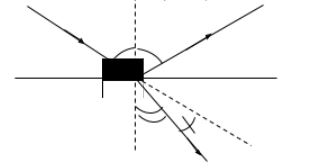
\includegraphics[scale=0.9]{../figs//VN11-2021-PH-TP028-03.JPG}
			\end{center}
		\end{enumerate}
	}
	
	\item \mkstar{2} [15]
	
	\cauhoi{
		Tia sáng đi từ nước có chiết suất $n_1 =\dfrac{4}{3}$ sang thủy tinh có chiết suất $n_2 = \text{1,5}$. Tính góc khúc xạ và góc lệch $D$ tạo bởi tia khúc xạ và tia tới, biết góc tới $i = 30^\circ$.
		
	}
	
	\loigiai{
		
		Ta có: 
		
		$$n_1 \sin i= n_2 \sin r \Rightarrow  r = \text{26,38}^\circ.$$
		
		Góc khúc xạ và góc lệch $D$ tạo bởi tia khúc xạ và tia tới
		
		$$D= i-r =\text{3,61}^\circ.$$
		
	}
	\item \mkstar{2} [35]
	
	\cauhoi{
		
		Một tia sáng từ không khí gặp khối nhựa trong suốt có chiết suất $n = \sqrt 2$ với góc tới $45^\circ$. Một phần của tia sáng bị phản xạ, một phần bị khúc xạ. Tính góc khúc xạ và góc hợp bởi tia khúc xạ và tia phản xạ. 
		
	}
	
	\loigiai{
		
		Ta có: 
		
		$$\dfrac{\sin i}{\sin r} = n_{21} \Rightarrow r =30^\circ.$$
		
		Góc phản xạ $i' = i =45^\circ.$ 
		
		Góc hợp bởi giữa tia khúc xạ và tia phản xạ
		
		$$\beta = 180^\circ -i' -r =105^\circ.$$
	}
	
	\item \mkstar{3} [37]
	
	\cauhoi{
		
		Một tia sáng đi từ thủy tinh có chiết suất bằng $\sqrt 3$  đến mặt phân cách giữa thủy tinh với không khí dưới góc tới $i=30^\circ$.
		
		\begin{enumerate}[label=\alph*)]
			\item Tính góc khúc xạ ra không khí.
			\item Tính góc tới $i$ để không có tia sáng ló ra không khí. 
		\end{enumerate}
		
		
	}
	
	\loigiai{
		
		\begin{enumerate}[label=\alph*)]
			\item Góc khúc xạ ra không khí 
			
			$$ \dfrac{\sin i}{\sin r} = \dfrac{n_2}{n_1} \Rightarrow r =60^\circ$$
			
			\item Để góc tới $i$ để không có tia sáng ló ra không khí 
			
			$$\sin i_\text{gh} = \dfrac{n_2}{n_1}.$$
			
			Suy ra: $i_\text{gh} = \text{35,26}^\circ$ nên $i \geq \text{35,26}^\circ$ 
		\end{enumerate}
		
		
	}
	
	\item \mkstar{3} [34]
	
	\cauhoi{
		Một tia sáng truyền từ không khí vào nước có chiết suất $\dfrac{4}{3}$ với góc tới $60^\circ$.
		
		\begin{enumerate}[label=\alph*)]
			\item Tìm góc khúc xạ.
			\item Tìm góc lệch $D$ giữa tia tới và tia khúc xạ.
			\item Tìm góc $\alpha$ tạo bởi tia phản xạ và tia khúc xạ. Vẽ hình minh họa lời giải.
		\end{enumerate}
	}
	
	\loigiai{
		
		\begin{enumerate}[label=\alph*)]
			\item Góc khúc xạ
			
			$$n_1 \sin i=n_2 \sin r \Rightarrow  r = \text{40,5}^\circ.$$
			
			\item Góc lệch $D$ giữa tia tới và tia khúc xạ
			
			$$D = i-r = \text{19,5}^\circ.$$
			
		 
		
		
			\item Ta có 
			
			\begin{center}
				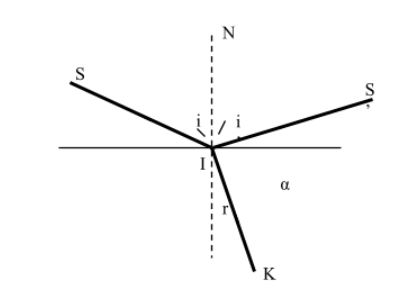
\includegraphics[scale=0.9]{../figs//VN11-2021-PH-TP028-04.JPG}
			\end{center}
		
			Trên hình vẽ ta thấy:
			
			$$i = i’= 60^\circ  \Rightarrow  \alpha = 180^ \circ - (60+ \text{40,5}) = \text{79,5}^\circ.$$
			
		\end{enumerate}
	}
	\item \mkstar{3} [15]
	
	\cauhoi{
		Một tia sáng đơn sắc đi từ môi trường trong suốt có chiết suất $n$ ra không khí với góc tới $i = 45^\circ$. Phần lớn ánh sáng bị khúc xạ, một phần nhỏ bị phản xạ. Gọi $\alpha$ là góc hợp giữa tia phản xạ với tia khúc xạ và $D$ là góc lệch (góc hợp bởi tia khúc xạ và đường kéo dài của tia tới). Cho biết: $\alpha = 4D$.
		
		\begin{enumerate}[label=\alph*)]
			\item Vẽ đường đi của các tia sáng và tìm chiết suất $n$.
			\item Cho tốc độ truyền của ánh sáng trong chân không bằng $c = 3 \cdot 10^8\ \text{m/s}$. Hãy tìm tốc độ truyền của ánh sáng trong môi trường chiết suất $n$.
		\end{enumerate}
		
	}
	\loigiai{
		
		\begin{enumerate}[label=\alph*)]
			\item Ta có:
			
			$$D =r -i$$ 
			
			và $\alpha = 180^\circ -i -r$.
			
			Mà $\alpha =4D$ suy ra $r=63^\circ$.
			
			Ta lại có:
			
			$$n\sin i = \sin r \Rightarrow n \approx \text{1,26}.$$
			\item Tốc độ truyền của ánh sáng trong môi trường chiết suất $n$
			
			$$v = \dfrac{c}{n} = \text{2,38} \cdot 10^8\ \text{m/s}.$$
			
		\end{enumerate}
	}
	\item \mkstar{3} [16]

	\cauhoi{
	Chiếu một tia sáng đơn sắc từ không khí đến gặp mặt phân cách của một chất trong suốt có chiết suất bằng $\sqrt 3$ với góc tới $60^\circ$.
	
	\begin{enumerate}[label=\alph*)]
		\item Tìm góc khúc xạ.
		\item Nếu chiếu tia sáng nói trên đi từ môi trường chiết suất bằng $\sqrt 3$ ở trên ra môi trường không khí với góc tới như trên thì có tia khúc xạ không? Tại sao?
	\end{enumerate}
	
	}
	\loigiai{
	
	\begin{enumerate}[label=\alph*)]
		\item Góc khúc xạ
		
		$$n_1 \sin i = n_2\sin r \Rightarrow r =30^\circ.$$
		
		
		\item 
		Ta có
		
		$$\sin_\text{igh} = \dfrac{n_2}{n_1} = \dfrac{1}{\sqrt 3} \Rightarrow i_\text{gh} \approx 35^\circ 15'$$
		
		Vì thỏa 2 điều kiện:
		
		Điều kiện 1: $$n_1 > n_2.$$
		
		Điều kiện 2: $$i > i_\text{gh}$$
		
		$\Rightarrow$ Có xảy ra hiện tượng phản xạ toàn phần, không có tia khúc xạ ra không khí.
		
	\end{enumerate}
}

		\item \mkstar{3} [23]
		
		\cauhoi{
			
			Một cái gậy thẳng dài $\SI{1,8}{m}$ cắm thẳng đứng ở đáy hồ. Gậy nhô lên khỏi mặt nước $\SI{0,6}{m}$. Ánh sáng Mặt Trời chiếu xuống hồ theo phương hợp với pháp tuyến của mặt nước một góc $45^\circ$. Tìm chiều dài bóng của gậy in trên đáy hồ. (Cho $n_\text{nước} = \dfrac{4}{3}$, $n_\text{kk} = 1$)
			
			
		}
		
		\loigiai{
			
			\begin{center}
				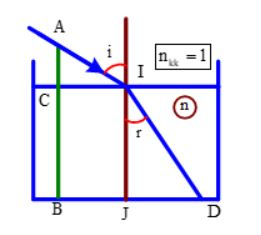
\includegraphics[scale=0.9]{../figs//VN11-2021-PH-TP028-06.JPG}
			\end{center}
		
		$$\tan 45^\circ = \dfrac{CI}{AI} \Rightarrow CI = \SI{0,6}{m}.$$
		
		Ta có:
		
		$$n_1 \sin i = n_2 \sin r \Rightarrow r = \text{32,03}^\circ.$$
		
		Lại có:
		
		$$\tan \text{32,03}^\circ = \dfrac{JD}{JI} \Rightarrow JD = \SI{0,75}{m}.$$
		
		Bóng cọc dưới đáy hồ là
		
		$$\text{0,6}+ \text{0,75}= \SI{1,35}{m}.$$
}
		
		\item \mkstar{3} [27]
	
	\cauhoi{
		Chiếu một tia sáng đơn sắc từ không khí vào khối thuỷ tinh chiết suất $n = \text{1,52}$. 
		\begin{enumerate}[label=\alph*)]
			\item Tính góc tới, biết góc khúc xạ là $25^\circ$. 
			\item Nếu tia tới hợp với mặt phân cách giữa không khí và thủy tinh một góc $30^\circ$ thì góc lệch giữa tia khúc xạ với và tia tới là bao nhiêu?
		\end{enumerate}
		
	}
	\loigiai{
		
		\begin{enumerate}[label=\alph*)]
			\item Ta có:
			
			$$n_1 \sin i = n_2 \sin r \Rightarrow i = 40^\circ.$$
			 
			\item Nếu tia tới hợp với mặt phân cách giữa không khí và thủy tinh một góc $30^\circ$ thì $i =60^\circ$.
			
			Ta có:
			
			$$n_1 \sin i = n_2 \sin r \Rightarrow i = 35^\circ.$$
		
			Vậy $D= i - r = 25^\circ.$
			
		\end{enumerate}
	}

		\item \mkstar{3} [28]
		
		\cauhoi{ 
			\begin{minipage}[l]{11cm}
				\begin{enumerate}[label=\alph*)]
					\item Một tia sáng đi từ không khí vào thủy tinh dưới góc tới bằng $65^\circ$. Biết thủy tinh có chiết suất là 1,52. Tính góc lệch giữa phương của tia tới và tia khúc xạ.
					\item Một người đang đứng dưới bể nước có con cá ở vị trí được biểu
					diễn như hình vẽ. Do hiện tượng khúc xạ ánh sáng, người sẽ không nhìn thấy con cá ở vị trí thực sự của nó và ngược lại, con cá cũng sẽ không nhìn thấy mắt người ở vị trí thực sự của nó. Hãy cho biết:
					
					Người sẽ nhìn thấy con cá ở vị trí a hay b ?
					
					Con cá sẽ nhìn thấy mắt người ở vị trí c hay d ?
					
				\end{enumerate}
			\end{minipage}
			\begin{minipage}[r]{5cm}
				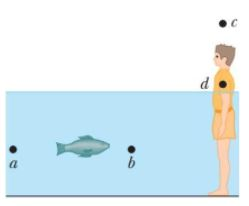
\includegraphics[scale=0.9]{../figs//VN11-2021-PH-TP028-08.JPG}
			\end{minipage}
		}
		\loigiai{
			
			\begin{enumerate}[label=\alph*)]
				\item Ta có:
				
				Góc khúc xạ:
				
				$$n_1 \sin i  = n_2 \sin r \Rightarrow r \approx 37^\circ.$$
				 
				Góc lệch giữa phương tia tới và tia khúc xạ: $$D = i - r = 28^\circ.$$
		
				\item 
				
				
				
				Người sẽ nhìn thấy con cá ở vị trí a. 
				
				Con cá sẽ nhìn thấy mắt người ở vị trí c.
				
				\begin{center}
					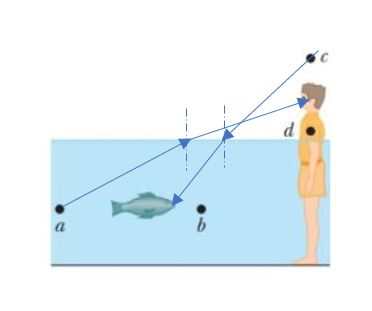
\includegraphics[scale=0.9]{../figs//VN11-2021-PH-TP028-09.JPG}
				\end{center}
				
			\end{enumerate}
		}
	
		\item \mkstar{3} [26]
	
	\cauhoi{
		\begin{minipage}{10cm}
			Đèn Moser (Moser’s Lamp) là một phát minh vô cùng ý nghĩa của một kỹ sư người Brazil, Alfredo Moser phát minh vào năm 2002. Ông đã dùng các chai nhựa dẻo đổ đầy nước và một ít chất tẩy trắng, gắn chúng vào các lỗ hổng trên trần nhà để chiếu sáng căn phòng của ông và hiện giờ ý tưởng này đã lan rộng trên khắp thế giới. Phương pháp này đã đem đến nguồn cung cấp năng lượng sạch, không tạo khí thải CO2 và thân thiện với môi trường. Đặc biệt, hàng triệu người dân nghèo, vốn phải sống trong các ngôi nhà ổ chuột nhỏ hẹp với hệ thống cửa sổ thiếu hợp lý, sử dụng phương tiện chiếu sáng chủ yếu là đèn dầu (cho ánh sáng yếu và sinh ra nhiều khí độc), nay đã được hưởng lợi từ phương pháp lấy năng lượng ánh sáng Mặt Trời này của Moser. Hình bên là nguyên lý hoạt động của đèn này. Hãy trả lời các câu hỏi bên dưới từ những thông tin đã cho.
		\end{minipage}
		\begin{minipage}[r]{5cm}
			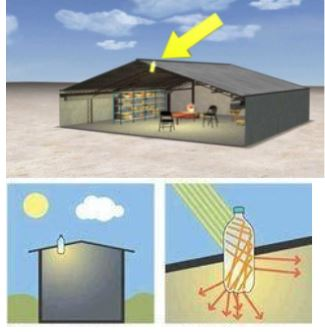
\includegraphics[scale=0.9]{../figs//VN11-2021-PH-TP028-07.JPG}
		\end{minipage}
		
		
		
		\begin{enumerate}[label=\alph*)]
			\item Những hiện tượng quang học chủ yếu nào đã xảy ra trong quá trình sử dụng đèn Moser?
			\item Để tia sáng từ Mặt Trời khi đi vào trong chai nước có thể lọt hết vào nhà thì các tia sáng trong chai nước tới gặp thành bên kia của chai phải có góc tới ít nhất là bao nhiêu? Cho biết chiết suất của nước là 4/3.
			\item Vì sao người nghèo “được hưởng lợi từ phương pháp lấy năng lượng từ ánh sáng Mặt Trời của Moser”? (Cần nêu được tối thiểu 2 lý do)
		\end{enumerate}
	}
	
	\loigiai{
		
		\begin{enumerate}[label=\alph*)]
			\item Những hiện tượng quang học chủ yếu: 
			
			+ Khúc xạ ánh sáng.
			
			+ Phản xạ toàn phần.
			
			\item Để toàn bộ tia sáng có thể lọt vào nhà thì các tia sáng trong chai nước tới gặp thành bên kia của chai phải có góc tới ít nhất là $i \geq i_\text{gh}$ với
			
			
			$$\sin i_\text{gh} = \dfrac{n_2}{n_1} = \dfrac{3}{4} \Rightarrow i_\text{gh} \approx \text{48}^\circ 35'.$$
			
			\item Người nghèo “được hưởng lợi từ phương pháp lấy năng lượng từ ánh sáng Mặt Trời của Moser” vì
			
			+ Đem đến nguồn cung cấp năng lượng sạch, không tạo khí thải $CO_2$ và thân thiện với môi trường.
			
			+ Tiết kiệm chi phí lắp đặt.
			
			
		\end{enumerate}
		
	}
\end{enumerate}	
\whiteBGstarEnd
	\stopcontents[mychapters]
	
\setcounter{mychapter}{26}
	\mychapter{Phản xạ toàn phần}
	\startcontents[mychapters]
	\printcontents[mychapters]{}{0}{\setcounter{tocdepth}{1}}
	\whiteBGstarBegin
\setcounter{section}{0}

\begin{enumerate}[label=\bfseries Câu \arabic*:]
	
	\item \mkstar{2} [21]
	
	\cauhoi{
		Cho một tia sáng đi từ nước $\left(n = \dfrac{4}{3}\right)$ ra không khí. Sự phản xạ toàn phần xảy ra khi góc tới thỏa mãn:
		
		\begin{mcq}(4)
			\item $i < 49^\circ$.	
			\item $i > 42^\circ$.	
			\item $i > 49^\circ$.	
			\item $i > 43^\circ$
		\end{mcq}
	}
	
	\loigiai{
		\textbf{Đáp án: C.}
		
		Ta có
		
		$$\sin i_\text{gh} =\dfrac{n_2}{n_1} = \dfrac{3}{4} \Rightarrow i_\text{gh} = \text{48,59}^\circ.$$
		
		Để xảy ra hiện tượng phản xạ toàn phần: $i \geq i_\text{gh}$
		
		Suy ra: $i \geq \text{48,59}^\circ$
	}
	
	\item \mkstar{1} [18]
	
	\cauhoi{
		
		Lúc trời nắng, mặt đường nhựa khô ráo, nhưng nhìn từ xa ta thấy mặt đường có vẻ bị ướt nước đó là kết quả của hiện tượng gì? Tại sao có hiện tượng đó xảy ra?
		
	}
	
	\loigiai{
		
		Mặt đường nhựa nóng, không khí tại gần mặt đất có nhiệt độ cao hơn không khí trên cao, dẫn đến chiết suất không khí tăng theo độ cao, các tia sáng từ bầu trời xanh có thể được khúc xạ toàn phần đến mắt người quan sát. Do không khí luôn có các dòng đối lưu gây nhiễu loạn chiết suất, hình ảnh thu được luôn dao động như khi nhìn hình ảnh bầu trời phản xạ từ mặt nước vậy nên ta có thể nhìn như thấy vũng nước trên đường. 
		
	}
	
	\item \mkstar{1} [14]
	
	\cauhoi{
		
		Nêu công dụng của cáp quang.
		
	}
	
	\loigiai{
		Ứng dụng của cáp quang:
		
		Trong công nghệ thông tin, cáp quang được dùng để truyền thông tin, dữ liệu dưới dạng tín hiệu ánh sáng.
		
		Trong nội soi y học.
	}
		\item \mkstar{1} [15]
		
		\cauhoi{
			
		Ngày nay, cáp quang được sử dụng rộng rãi (thay thế cáp đồng) để truyền tín hiệu trong viễn thông, em hãy cho biết cáp quang là ứng dụng của hiện tượng vật lý nào? Ưu điểm và nhược điểm của cáp quang? 
			
			
		}
		
		\loigiai{
			
			Cáp quang là ứng dụng của hiện tượng phản xạ toàn phần.
					
		*Ưu điểm:
		
		- Mỏng, dung lượng tải cao hơn cho phép nhiều kênh đi qua cáp của bạn.
		
		- Suy giảm tín hiệu ít - tín hiệu bị mất trong cáp quang ít hơn trong cáp đồng.
			
			
		*Nhược điểm:
		
		- Nối cáp khó, phải thẳng, không được gập. 
		
		- Chi phí cao.
			
		}

	
	
	\item \mkstar{1} [7]
	
	\cauhoi{
		Thế nào là hiện tượng phản xạ toàn phần? Nêu điều kiện để có phản xạ toàn phần.	
	}
	
	\loigiai{
		
		Hiện tượng phản xạ toàn phần là hiện tượng phản xạ toàn bộ tia sáng tới,    xảy ra ở mặt phân cách giữa hai môi trường trong suốt.
		
		Điểu kiện xảy ra phản xạ toàn phần: 
		
		$$n_1 >n_2.$$
		
		$$i \geq i_\text{gh}.$$
		
	}
	
	\item \mkstar{2} [36]
	
	\cauhoi{
		
		Chiếu một tia sáng đến mặt tiếp xúc nước - không khí. Tìm góc tới để xảy ra hiện tượng phản xạ toàn phần. (Biết chiết suất của nước đối với tia sáng là $\dfrac{4}{3}$)
		
		
	}
	
	\loigiai{
		
		Ta có
		
		$$\sin i_\text{gh} =\dfrac{n_2}{n_1} = \dfrac{3}{4} \Rightarrow i_\text{gh} = \text{48,59}^\circ.$$
		
		Để xảy ra hiện tượng phản xạ toàn phần: $i \geq i_\text{gh}$
		
		Suy ra: $i \geq \text{48,59}^\circ$
		
	}
	\item \mkstar{2} [24]
	
	\cauhoi{
		
		Chiếu tia sáng từ nước vào không khí sao cho tia sáng tới hợp với mặt nước một góc $60^\circ$. Cho chiết suất nước là $\dfrac{4}{3}$. Hỏi có xảy ra hiện tượng phản xạ toàn phần không? 
		
	}
	\loigiai{
		
		Ta có: 
		
		$$i =90^\circ -60^\circ =30^\circ.$$
		
		$$\sin i_\text{gh} = \dfrac{n_2}{n_1} \Rightarrow i_\text{gh} = \text{48,59}^\circ.$$
		
		Lại có:
		
		$$n_2 > n_1 \ \text{và} i<i_\text{gh}.$$
		
		Nên xảy ra hiện tượng khúc xạ ánh sáng.
	}
	
	\item \mkstar{2} [18]
	
	\cauhoi{
		
		Một tia sáng truyền từ một môi trường trong suốt có chiết suất 1,5 sang không khí. Tính góc tới của tia sáng để có tia ló ra không khí? Biết chiết suất không khí bằng 1.
		
	}
	
	\loigiai{
		
		Ta có:
		
		$$\sin i_\text{gh}= \dfrac{n_2}{n_1}= \text{0,67}\Rightarrow i_\text{gh} = \text{41,8}.$$
		
		Để có tia ló ra không khí  $i < i_\text{gh}$
		
		
	}
	\item \mkstar{3} [10]
	
	\cauhoi{
		Một tia sáng truyền từ môi trường có chiết suất $n_1 = \sqrt 6$, đến gặp mặt phân cách của môi trường thứ hai có chiết suất $n_2 = \sqrt 2$.
		  
		\begin{enumerate}[label=\alph*)]
			\item Tìm điều kiện của góc tới để không có tia sáng nào ra môi trường thứ hai.
			\item Góc tới $i$ phải bằng bao nhiêu để khi truyền qua mặt phân cách, tia sáng bị lệch so với phương ban đầu một góc bằng $i$?
		\end{enumerate}
	}
	
	\loigiai{
				
		\begin{enumerate}[label=\alph*)]
			\item ABC.Để không có tia sáng ló ra môi trường 2 $\Rightarrow$ hiện tượng phản xạ tòan phần
			
			$$\sin i_\text{gh} =\dfrac{n_2}{n_1} = \text{0,577} \Rightarrow i_\text{gh}=\text{35,24}^\circ.$$
			
			$$\Rightarrow i \geq \text{35,24}^\circ.$$
			
			\item Ta có:
			
			$$n_1 \sin i = n_2 \sin r$$
			
			$$\Rightarrow n_1 \sin i = n_2 \sin 2i$$
			
			$$n_1 \sin i = n_2 2\sin i \cos i.$$
			
			$$\Rightarrow \cos i  = \dfrac{n_1}{2n_2} = \dfrac{\sqrt 3}{2}\Rightarrow i =30^\circ.$$
			
			
		\end{enumerate}
	}
	
		\item \mkstar{3} [20]
	
	\cauhoi{
		
	Một tia sáng truyền từ môi trường trong suốt có chiết suất $n$ ra không khí, dưới góc tới $30^\circ$ thì tia khúc xạ ra không khí có hướng lệch so với tia tới một góc bằng $15^\circ$.
	
	\begin{enumerate}[label=\alph*)]
		\item Xác định giá trị chiết suất $n$ của môi trường.
		\item Để không có tia khúc xạ ra không khí thì phải tăng góc tới ít nhất bao nhiêu độ? 
	\end{enumerate} 
	
		
	}
	
	\loigiai{
		
	
		\begin{enumerate}[label=\alph*)]
			\item Chiết suất $n$ của môi trường
			
			$$D = r - i  \Rightarrow r = 45^\circ.$$  
			
			$$n \sin i = \sin r \Rightarrow n = \sqrt 2.$$           
			                       
			
			\item 
			Ta có:
			
			$$\sin i_\text{gh} = \dfrac{1}{n} \Rightarrow i_\text{gh} = 45^\circ.$$
			     
			để xảy ra phản xạ toàn phần thì $i \geq i_\text{gh} \Leftrightarrow i \geq 45^\circ.$
			
			$\Rightarrow$ góc tới tăng ít nhất $15^\circ$. 
			        
		\end{enumerate} 
	}
	

	
	\item \mkstar{3} [23]
	
	\cauhoi{
		
		Tia sáng đi từ thuỷ tinh có chiết suất $\sqrt 3$ đến môi trường chất lỏng có chiết suất $\sqrt 2$.
		
		\begin{enumerate}[label=\alph*)]
			\item Tìm góc giới hạn phản xạ toàn phần.
			\item Cho góc tới $45^\circ$ thì có tia sáng đi vào chất lỏng không? Nếu có, tìm góc khúc xạ.
		\end{enumerate}
		
	}
	
	\loigiai{
		
		\begin{enumerate}[label=\alph*)]
			\item Giới hạn phản xạ toàn phần
			
			$$\sin i_\text{gh} = \dfrac{n_2}{n_1} \Rightarrow i_\text{gh} = \text{54,73}^\circ.$$
			
			\item Ta có:
			
			$i < i_\text{gh}$ nên có tia khúc xạ.
			
			$$n_1 \sin i = n_2 \sin r \Rightarrow r =60^\circ.$$
			
		\end{enumerate}
	}
	
	
	
	\item \mkstar{3} [33]
	
	\cauhoi{
		Một tia sáng truyền từ môi trường có chiết suất $\sqrt 2$ hướng tới mặt phân cách với không khí.
		
	\begin{enumerate}[label=\alph*)]
		\item Tính góc giới hạn phản xạ toàn phần.
		\item Nếu góc tới của tia sáng là $48^\circ$ thì tia sáng có bị phản xạ toàn phần không? Tại sao?
	\end{enumerate}
	}
	
	\loigiai{
	
	\begin{enumerate}[label=\alph*)]
		\item Góc giới hạn phản xạ toàn phần
		
		$$\sin i_\text{gh} = \dfrac{n_2}{n_1} \Rightarrow i_\text{gh} = 45^\circ.$$
		
		\item Nếu góc tới của tia sáng là $48^\circ$ thì tia sáng xảy phản xạ toàn phần vì $i \geq i_\text{gh}$.
	\end{enumerate}
	
	
	}
	

\end{enumerate}	
\whiteBGstarEnd
	\stopcontents[mychapters]
	
\chapter[\textbf{Ôn tập: Chương VI. Khúc xạ ánh sáng}]{Ôn tập: Chương VI. Khúc xạ ánh sáng}
	\startcontents[chapters]
	\printcontents[chapters]{}{0}{\setcounter{tocdepth}{1}}
	\whiteBGstarBegin
\setcounter{section}{0}
\section{Khúc xạ ánh sáng}
\begin{enumerate}[label=\bfseries Câu \arabic*:]
	
	\item \mkstar{2} 
	
	\cauhoi{
		
		\textbf{(Đề chính thức của BGDĐT - 2018)} Chiết suất của nước và của thủy tinh đối với một ánh sáng đơn sắc có giá trị lần lượt là 1,333 và 1,532. Chiết suất tỉ đối của nước đối với thủy tinh ứng với ánh sáng đơn sắc này là
		\begin{mcq}(4)
			\item 0,199.			
			\item 0,870.			
			\item 1,433.			
			\item 1,149.
		\end{mcq}
	}
	
	\loigiai{
		\textbf{Đáp án: B.}
		
		Chiết suất tỉ đối của nước so với thủy tinh ứng với ánh sáng đơn sắc 
		
		$$ n = \dfrac{\text{1,333}}{\text{1,532}} = \text{0,87}.$$
		
		
		
	}
	
	\item \mkstar{2} 
	
	\cauhoi{
		
		(Đề chính thức của BGDĐT - 2018) Chiếu một tia sáng đơn sắc từ không khí tới mặt nước với góc tới $60^\circ$, tia khúc xạ đi vào trong nước với góc khúc xạ là $r$. Biết chiết suất của không khí và của nước đối với ánh sáng đơn sắc này lần lượt là 1 và 1,333. Giá trị của $r$ là
	\begin{mcq}(4)
	\item $\text{37,97}^\circ$.			
	\item $\text{22,03}^\circ$.			
	\item $\text{40,52}^\circ$.			
	\item $\text{19,48}^\circ$.
	\end{mcq}
		
	}
	
	\loigiai{
		\textbf{Đáp án: C.}
		
		Giá trị của góc khúc xạ r được xác định bởi biểu thức :
		
		$$ \dfrac{\sin i}{\sin r} = n \Rightarrow r = \text{40,52}^\circ.$$
	}
	
	\item \mkstar{2} 
	
	\cauhoi{
		
		Tính tốc độ của ánh sáng trong thủy tinh. Biết thủy tinh có chiết suất $n = \text{1,6}$ và tốc độ ánh sáng trong chân không là $c = 3\cdot 10^8\ \text{m/s}$.
		\begin{mcq}(4)
			\item 2,23$\cdot 10^8\ \text{m/s}$.		
			\item 1,875$\cdot 10^8\ \text{m/s}$. 		
			\item 2,75$\cdot 10^8\ \text{m/s}$.		
			\item 1,5$\cdot 10^8\ \text{m/s}$.
		\end{mcq}
	}
	
	\loigiai{
				
		\textbf{Đáp án: B.}
		
		Tốc độ của ánh sáng trong thủy tinh
		
		$$n = \dfrac{c}{v} \Rightarrow v = \dfrac{c}{n} = \text{1,875} \cdot 10^8\ \text{m/s}.$$
		
	}
	
	
	\item \mkstar{2}
	
	\cauhoi{
		
		Một tia sáng truyền từ môi trường A vào môi trường B dưới góc tới $6^\circ$ thì góc khúc xạ là $8^\circ$. Tính tốc độ ánh sáng trong môi trường A. Biết tốc độ ánh sáng trường môi trường B là 2$\cdot 10^5$ km/s.
		\begin{mcq}(4)
			\item 2,25$\cdot 10^5$ km/s. 		
			\item 2,3$\cdot 10^5$ km/s.		
			\item l,5$\cdot 10^5$ km/s. 		
			\item 2,5$\cdot 10^5$ km/s.
		\end{mcq}
	}
	
	\loigiai{
		
		\textbf{Đáp án: C.}
		
		Ta có:
		
		$$\dfrac{v_1}{v_2} = \dfrac{n_2}{n_1} = \dfrac{\sin i}{\sin r} \Rightarrow v_1 = \text{1,5} \cdot 10^5\ \text{km/s}.$$
	}
	
	\item \mkstar{2}
	
	\cauhoi{
		
		Tia sáng đi từ nước có chiết suất $n_1 = \dfrac{4}{3}$ sang thủy tinh có chiết suất $n_2 = \text{1,5}$ với góc tới $i = 30^\circ$. Góc khúc xạ và góc lệch $D$ tạo bởi tia khúc xạ và tia tới lần lượt là
		\begin{mcq}(4)
			\item $\text{26,4}^\circ$ và  $\text{3,6}^\circ$.	
			\item $\text{50,34}^\circ$ và  $\text{9,7}^\circ$.		
			\item $\text{34,23}^\circ$ và  $\text{4,23}^\circ$.			
			\item $\text{76,98}^\circ$ và  $\text{47}^\circ$.	
		\end{mcq}
	}
	
	\loigiai{
		
		\textbf{Đáp án: A.}
		
		Ta có:
		
		$$n_1 \sin i = n_2 \sin r \Rightarrow \sin r = \dfrac{n_1 \sin i}{n_2} \Rightarrow r = \text{26,39}^\circ.$$
		
		Lại có:
		
		$$D = i -r \approx \text{3,6}^\circ.$$
		
	}
		\item \mkstar{2}
	
	\cauhoi{
		
		Tia sáng truyền trong không khí tới gặp mặt thoáng của chất lỏng có chiết suất $n =\sqrt 3$. Nếu tia phản xạ và tia khúc xạ vuông góc với nhau thì góc tới bằng 
		\begin{mcq}(4)
			\item $30^\circ$.			
			\item $60^\circ$.			
			\item $75^\circ$.		
			\item $45^\circ$.
		\end{mcq}
	}
	\loigiai{
		
		\textbf{Đáp án: B.}
		
		Theo đầu bài, ta có:
		
		$$n_1 =1; n_2 = \sqrt 3.$$
		
		Gọi $i'$ là góc phản xạ, ta có:
		
		$$i' + r = 90^\circ \Rightarrow i + r =90^\circ.$$
		
		Do góc phản xạ bằng góc tới.
		
		Theo định luật khúc xạ ánh sáng, ta có:
		
		$$n_1 \sin i = n_2 \sin r \Rightarrow \tan i = \sqrt 3 \Rightarrow i =60^\circ.$$
		
	}
	\item \mkstar{2}
	
	\cauhoi{
		
		Tia sáng truyền trong không khí tới gặp mặt thoáng của chất lỏng có chiết suất $n = \text{1,6}$. Nếu tia phản xạ và tia khúc xạ hợp với nhau một góc $100^\circ$ thì góc tới bằng
		\begin{mcq}(4)
			\item $36^\circ$.			
			\item $60^\circ$.				
			\item $72^\circ$.				
			\item $51^\circ$.
		\end{mcq}
	}
	\loigiai{
		
		\textbf{Đáp án: D.}
		
		\begin{center}
			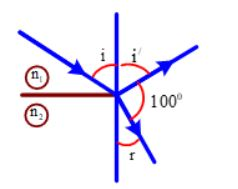
\includegraphics[scale=0.8]{../figs/VN11-2021-PH-TP030-04.JPG}
		\end{center}
	
	Ta có:
	
	$$r = 80^\circ - i .$$
	
	Theo định luật khúc xạ ánh sáng
	
	$$n_1 \sin i = n_2 \sin r \Rightarrow i = \text{50,96}^\circ.$$
	}
	\item \mkstar{3}
	
	\cauhoi{
		
		Một thợ lặn ở dưới nước nhìn thấy Mặt Trời ở độ cao $60^\circ$ so với đường chân trời. Biết chiết suất của nước là $n = \dfrac{4}{3}$. Tính độ cao thực của Mặt Trời so với đường chân trời.
		\begin{mcq}(4)
			\item $38^\circ$.			
			\item $60^\circ$.				
			\item $72^\circ$.				
			\item $48^\circ$.
		\end{mcq}
	}
	\loigiai{
		
		\textbf{Đáp án: D.}
		
		\begin{center}
			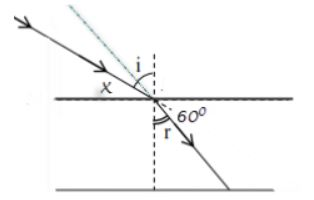
\includegraphics[scale=0.8]{../figs/VN11-2021-PH-TP030-05.JPG}
		\end{center}
	
	Hướng của Mặt Trời mà người thợ lặn nhìn thấy là hướng của các tia sáng khúc xạ vào nước.
	
	$$r = 90^\circ - 60^\circ =30^\circ.$$
	
	Định luật khúc xạ ánh sáng
	
	$$\sin i - n \sin r \Rightarrow i =42^\circ.$$
	
	Độ cao thực của đường chân trời so với mặt trời là 
	
	$$\alpha  = 90^\circ - i  = 48^\circ.$$
		
	}
	\item \mkstar{3}
	
	\cauhoi{
		
		Ba môi trường trong suốt (1), (2), (3) có thể đặt tiếp giáp nhau. Với cùng góc tới $i = 60^\circ$; nếu ánh sáng truyền từ (1) vào (2) thì góc khúc xạ là $45^\circ$; nếu ánh sáng truyền từ (1) vào (3) thì góc khúc xạ là $30^\circ$. Nếu ánh sáng truyền từ (2) vào (3) vẫn với góc tới $i$ thì góc khúc xạ gần giá trị nào nhất sau đây?
		\begin{mcq}(4)
			\item $36^\circ$.			
			\item $60^\circ$.				
			\item $72^\circ$.				
			\item $51^\circ$.
		\end{mcq}
	}
	\loigiai{
		
		\textbf{Đáp án: A.}
		
		Từ (1) đến (2):
		
		$$\dfrac{\sin 60^\circ}{\sin 45^\circ} = \dfrac{n_2}{n_1}$$
		
		Từ (1) đến (3):
		
		$$\dfrac{\sin 60^\circ}{\sin 30^\circ} = \dfrac{n_3}{n_1}$$
		
		Suy ra
		
		$$\dfrac{\sin 45^\circ}{\sin 30^\circ} = \dfrac{n_3}{n_2}$$
		
		Mà từ (2) đến (3):
		
		$$\dfrac{\sin 60^\circ}{\sin r} = \dfrac{n_3}{n_2}$$
		
		Vậy:
		
		$$\dfrac{\sin 45^\circ}{\sin 30^\circ} = \dfrac{\sin 60^\circ}{\sin r} \Rightarrow r =38^\circ.$$
		
		
		
	}



\end{enumerate}

\section{Phản xạ toàn phần}
\begin{enumerate}[label=\bfseries Câu \arabic*:]
	
	\item \mkstar{2} 
	
	\cauhoi{
		
		\textbf{(Đề chính thức của BGD-ĐT - 2018)} Chiếu một tia sáng đơn sắc từ trong nước tới mặt phân cách với không khí. Biết chiết suất của nước và của không khí đối với ánh sáng đơn sắc này lần lượt là 1,333 và 1. Góc giới hạn phản xạ toàn phần ở mặt phân cách giữa nước và không khí đối với ánh sáng đơn sắc này là 
		\begin{mcq}(4)
			\item 41,40$^\circ$.			
			\item 53,12$^\circ$.			
			\item 36,88$^\circ$.			
			\item 48,61$^\circ$.
		\end{mcq}
	}
	
	\loigiai{
		
		\textbf{Đáp án: D.}
		
		Góc giới hạn phản xạ toàn phần ở mặt phân cách giữa nước và không khí đối với ánh sáng đơn sắc này là
		
		$$\sin i_\text{gh} = \dfrac{1}{n} = \text{48,61}^\circ.$$
	}
	
	\item \mkstar{2}
	
	\cauhoi{
		Biết chiết suất của thủy tinh là 1,5 và của nước là $\dfrac{4}{3}$. Góc giới hạn phản xạ toàn phần khi ánh sáng truyền từ thủy tinh sang nước bằng
		\begin{mcq}(4)
			\item 46,8$^\circ$.			
			\item 72,5$^\circ$.			
			\item 62,7$^\circ$.			
			\item 41,8$^\circ$.
		\end{mcq}
	}
	\loigiai{
		
		\textbf{Đáp án: C.}
		
		Góc giới hạn phản xạ toàn phần ở mặt phân cách giữa thủy tinh sang nước đối với ánh sáng đơn sắc này là
		
		$$\sin i_\text{gh} = \dfrac{n_\text{nhỏ}}{n_\text{lớn}}  \Rightarrow i_\text{gh} = \text{62,7}^\circ.$$
	}

		
		\item \mkstar{2}
		
		\cauhoi{
			\begin{minipage}[l]{12cm}
				Một chùm tia sáng hẹp SI truyền trong mặt phẳng tiêt diện vuông góc của một khối trong suốt, đặt trong không khí, tam giác ABC vuông tại A với $\text{AB} = \text{1,2}\ \text{AC}$ như hình vẽ. Tia sáng phản xạ toàn phần ở mặt AC. Trong điều kiện đó, chiết suất n của khối trong suốt có giá trị như thế nào?
			\end{minipage}
			\begin{minipage}[r]{5cm}
				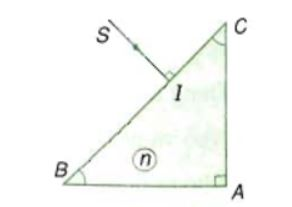
\includegraphics[scale=0.6]{../figs/VN11-PH-35-P-023-1-1.JPG}
			\end{minipage}
				
			\begin{mcq}(4)
				\item $n > \text{1,4}$.				
				\item $n < \text{1,41}$.
				\item $1 < n < \text{1,42}$.			
				\item $n > \text{1,3}$.
			\end{mcq}
		}
		\loigiai{
			
			\textbf{Đáp án: A.}
			
			Tam giác ABC vuông cân tại A.
			
			\begin{center}
				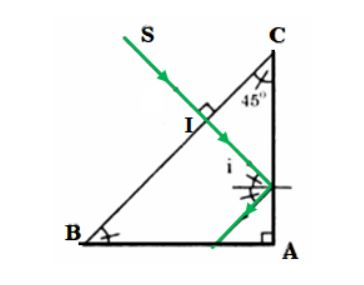
\includegraphics[scale=0.6]{../figs/VN11-2021-PH-TP030-02.JPG}
			\end{center}
			
			Góc B và góc C bằng $45^\circ.$
			
			Mà SI vuông góc BC. Tia sáng SI truyền thẳng vào môi trường trong suốt ABC mà không bị khúc xạ góc tới $i$ ở mặt phẳng BC:
			
			$$ i = 45^\circ \sin i = \sin 45^\circ = \dfrac{1}{\sqrt 2} $$
			
			
			Tia sáng phản xạ toàn phần ở mặt AC 
			
			$$\Rightarrow i \geq i_\text{gh} \Rightarrow \sin i \geq \sin i_\text{gh} = \dfrac{1}{n} \Rightarrow n \geq \sqrt 2.$$
			
			
		}
			\item \mkstar{3}
		
		\cauhoi{
			\begin{minipage}[l]{11cm}
				Một sợi quang hình trụ, lõi có chiết suất $n_1 = \text{1,50}$. Phần vỏ bọc có chiết suất $n_2 = \text{1,414}$. Chùm tia đi từ không khí tới hội tụ ở mặt trước của sợi với góc $2\alpha$ như hình vẽ. Giá trị lớn nhất của $\alpha$ để các tia sáng của chùm truyền đi được trong lõi gần giá trị nào nhất sau đây?
			\end{minipage}
			\begin{minipage}[r]{5cm}
				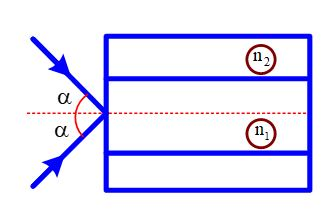
\includegraphics[scale=0.6]{../figs/VN11-PH-35-P-023-1-2.JPG}
			\end{minipage}		
			
			\begin{mcq}(4)
				\item 26$^\circ$.		
				\item 60$^\circ$.			
				\item 30$^\circ$.			
				\item 41$^\circ$.
			\end{mcq}
		}
		\loigiai{
			
			\textbf{Đáp án: C.}
			
			Điều kiện mọi tia sáng trong chùm đều truyền đi được trong ống là phải thỏa mãn điều kiện phản xạ toàn phần tại mặt phân cách của lõi trụ với vỏ bóc của nó.
			
			\begin{center}
				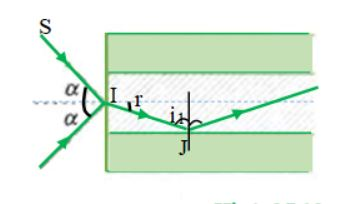
\includegraphics[scale=0.6]{../figs/VN11-2021-PH-TP030-01.JPG}
			\end{center}
		
			Điều kiện phản xạ toàn phần tại J là
			
			$$ i_1 \geq i_\text{gh} \Rightarrow \sin i_1 \geq \sin i_\text{gh} = \dfrac{n_2}{n_1}.$$
			
			Mặt khác:
			
			$$r=90^\circ - i_1 \Rightarrow \cos r = \sin i_1 \geq \dfrac{n_2}{n_1}.$$
			
			Áp dụng định luật khúc xạ tại mặt trước của ống quang ta được:
			
			$$\sin \alpha = n_1 \sin r = n_1 \sqrt{1- \cos^2 r} \leq n_1 \sqrt{1- \left(\dfrac{n_2}{n_1}\right)^2} \Rightarrow \alpha \leq 30^\circ.$$
		}
			\item \mkstar{3}
		
		\cauhoi{
			
			Một cái đinh được cắm vuông góc vào tâm O một tâm gỗ hình tròn có bán kính $R = 5\ \text{cm}$. Tấm gỗ được thả nổi trên mặt thoáng của một chậu nước. Đầu A của đỉnh trong nước. Cho chiết suất của nước là $n = \dfrac{4}{3}$. Để mắt không còn nhìn thấy đầu A của đỉnh thì khoảng cách OA lớn nhất là
			\begin{mcq}(4)
				\item 6,5 cm.			
				\item 7,2 cm.			
				\item 4,4 cm.			
				\item 5,6 cm.
			\end{mcq}
		}
		\loigiai{
			
			\textbf{Đáp án: C.}
			
			\begin{center}
				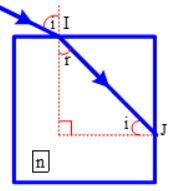
\includegraphics[scale=0.8]{../figs/VN11-2021-PH-TP030-03.JPG}
			\end{center}
		
		$$\dfrac{\sin i}{\sin r} = \dfrac{n_2}{n_1} \Rightarrow i = \text{48,59}^\circ.$$
		
		$$\text{OA} = \dfrac{\text{OI}}{\tan r} = \text{4,41}\ \text{cm}.$$
		}
		
\end{enumerate}
\whiteBGstarEnd
	\stopcontents[chapters]
	
\setcounter{mychapter}{27}
	\mychapter{Lăng kính}
	\startcontents[mychapters]
	\printcontents[mychapters]{}{0}{\setcounter{tocdepth}{1}}
	\whiteBGstarBegin
\setcounter{section}{0}
\begin{enumerate}[label=\bfseries Câu \arabic*:]
	
	\item \mkstar{1} [6]
	
	\cauhoi{
		Trình bày tác dụng của lăng kính đối với sự truyền ánh sáng qua nó. Xét hai trường hợp: Ánh sáng đơn sắc và ánh sáng trắng.
		
	}
	
	\loigiai{		
		
		- Tia sáng đơn sắc chiếu đến mặt bên của lăng kính, khi có tia ló ra khỏi lăng kính thì tia ló bao giờ cũng lệch về phía đáy lăng kính so với tia tới. 
		
		- Chùm ánh sáng trắng khi đi qua lăng kính sẽ bị phân tích thành nhiều chùm sáng đơn sắc khác nhau. 
		
	}
	
	
	\item \mkstar{1} [16]
	
	\cauhoi{
	
	Lăng kính là gì? Nêu các phần tử và đặc trưng quang học của lăng kính.
	
	}
	
	\loigiai{
		
		- Lăng kính là một khối chất trong suốt, đồng chất, thường có dạng lăng trụ tam giác.  
		
		- Các phần tử của lăng kính gồm: cạnh, đáy và hai mặt bên.  
		
		- Đặc trưng quang học của lăng kính gồm: góc chiết quang $A$ và chiết suất $n$.
		
	}

\end{enumerate}	
\whiteBGstarEnd
	\stopcontents[mychapters]
	
\setcounter{mychapter}{28}
	\mychapter{Thấu kính mỏng}
	\startcontents[mychapters]
	\printcontents[mychapters]{}{0}{\setcounter{tocdepth}{1}}
	\whiteBGstarBegin
\setcounter{section}{0}
\section{Lý thuyết: Thấu kính mỏng và tính chất quang học của thấu kính mỏng}
\begin{enumerate}[label=\bfseries Câu \arabic*:]
	
	\item \mkstar{1} [15]
	
	\cauhoi{
		
	Thấu kính mỏng là gì? Phân loại và nêu một số ứng dụng của thấu kính mỏng trong cuộc sống. 
		
	}
	
	\loigiai{
		
		- Thấu kính là một khối chất trong suốt giới hạn bởi hai mặt cong hoặc một mặt cong và một mặt phẳng.
		
		- Có hai loại: thấu kính hội tụ (rìa mỏng) và thấu kính phân kì (rìa dày).
		
		- Ứng dụng: kính khắc phục tật của mắt (kính cận, lão...), máy chiếu,...
	}
	
	\item \mkstar{1} [18]
	
	\cauhoi{
		Nêu tính chất quang học của quang tâm, tiêu điểm ảnh chính, tiêu điểm vật chính của thấu kính phân kỳ. Minh họa bằng đường truyền tia sáng cho mỗi trường hợp.
		
		
	}
	
	\loigiai{
		
		 Mọi tia sáng tới qua quang tâm O đều truyền thẳng qua thấu kính. Hình vẽ:
		 
		 \begin{center}
		 	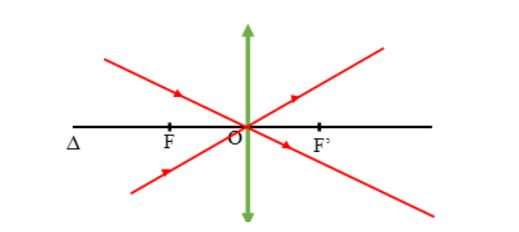
\includegraphics[scale=0.9]{../figs//VN11-2021-PH-TP028-10.JPG}
		 \end{center}
	 
	 	Mọi tia sáng tới song song với trục chính là tia ló sẽ qua tiêu điểm ảnh F’ ( đối với thấu kính hội tụ) hay có đường kéo dài qua tiêu điểm ảnh F’ ( đối với thấu kính phân kì). Hình vẽ:
	 	
	 	\begin{center}
	 		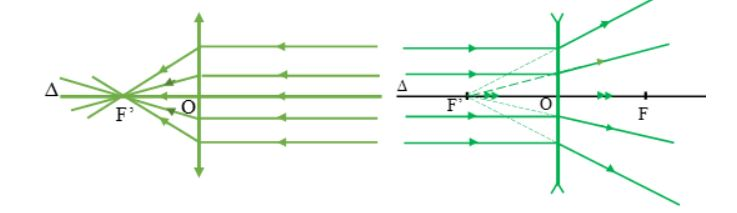
\includegraphics[scale=0.9]{../figs//VN11-2021-PH-TP028-11.JPG}
	 	\end{center}
 	
 		Mọi tia sáng tới qua tiêu điểm vật F (đối với thấu kính hội tụ) hay có đường kéo dài qua tiêu điểm vật F (đối với thấu kính phân kì) thì tia ló sẽ song song với trục chính. Hình vẽ:
 		
 		\begin{center}
 			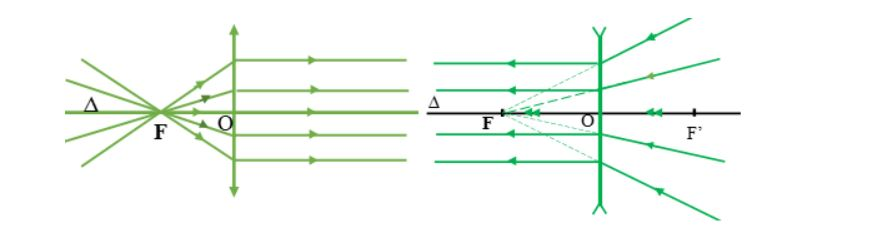
\includegraphics[scale=0.9]{../figs//VN11-2021-PH-TP028-12.JPG}
 		\end{center}
	}
	
	\item \mkstar{1} [20]
	
	\cauhoi{
		
		Vật thật đặt trước thấu kính phân kỳ sẽ cho ảnh có tính chất như thế nào?
		
	}
	
	\loigiai{		
		
	Thấu kính phân kì: vật thật luôn cho ảnh ảo, nhỏ hơn vật, cùng chiều vật.
		
	}
	
	

\end{enumerate}
\section{Lý thuyết: Đường đi của tia sáng qua thấu kính và vẽ ảnh tạo bởi thấu kính}
\begin{enumerate}[label=\bfseries Câu \arabic*:]
	
		\item \mkstar{1} [32]
	
	\cauhoi{
		
		Tìm hình vẽ đúng về đường truyền tia sáng qua quang tâm O của thấu kính
		
		\begin{mcq}(2)
			\item \begin{center}
				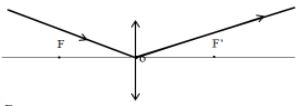
\includegraphics[scale=0.9]{../figs//VN11-2021-PH-TP028-14.JPG}
			\end{center}
			\item \begin{center}
				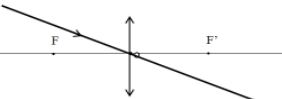
\includegraphics[scale=0.9]{../figs//VN11-2021-PH-TP028-15.JPG}
			\end{center}
			\item \begin{center}
				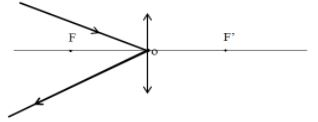
\includegraphics[scale=0.9]{../figs//VN11-2021-PH-TP028-16.JPG}
			\end{center}
			\item \begin{center}
				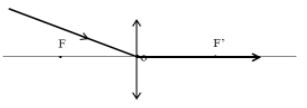
\includegraphics[scale=0.9]{../figs//VN11-2021-PH-TP028-17.JPG}
			\end{center}
			
		\end{mcq}
	}
	
	\loigiai{
		\textbf{Đáp án: B.}
	}
	\item \mkstar{1} [32]

	\cauhoi{

		Tìm hình vẽ đúng về đường truyền tia sáng qua các thấu kính sau:
		
		
		\begin{mcq}(2)
			\item \begin{center}
				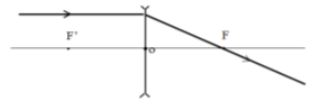
\includegraphics[scale=0.9]{../figs//VN11-2021-PH-TP028-18.JPG}
			\end{center}
			\item \begin{center}
				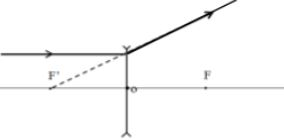
\includegraphics[scale=0.9]{../figs//VN11-2021-PH-TP028-19.JPG}
			\end{center}
			\item \begin{center}
				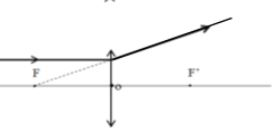
\includegraphics[scale=0.9]{../figs//VN11-2021-PH-TP028-20.JPG}
			\end{center}
			\item \begin{center}
				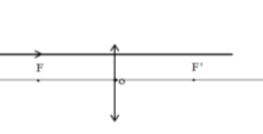
\includegraphics[scale=0.9]{../figs//VN11-2021-PH-TP028-21.JPG}
			\end{center}
			
		\end{mcq}
	}
		\loigiai{
			
			\textbf{Đáp án: B.}
		
	}
		\item \mkstar{2} [21]
	
	\cauhoi{
		Vật sáng AB đặt vuông góc với trục chính của thấu kính, cách thấu kính một khoảng $\SI{40}{cm}$ cho một ảnh trước thấu kính $\SI{20}{cm}$. Đây là
		
		\begin{mcq}(2)
			\item thấu kính hội tụ có tiêu cự $\SI{40}{cm}$.	
			\item thấu kính phân kì có tiêu cự $\SI{40}{cm}$.
			\item thấu kính hội tụ có tiêu cự $\SI{20}{cm}$.	
			\item thấu kính phân kì có tiêu cự $\SI{20}{cm}$.
		\end{mcq}
	}
	
	\loigiai{
		\textbf{Đáp án: B.}
		
		Ta có: $d = \SI{40}{cm}$.
		
		Do ảnh trước thấu kính nên $d'=-\SI{20}{cm}$ 
		
		$$\dfrac{1}{f} = \dfrac{1}{d} + \dfrac{1}{d'} = - \dfrac{1}{40} \Rightarrow f = -\SI{40}{cm}.$$
		
		Thấu kính đã cho là thấu kính phân kì do ảnh trước thấu kính và có $f = -\SI{40}{cm}$. 
	}
	
	\item \mkstar{1} [10]

\cauhoi{
	
	Thấu kính là gì? Khi vật sáng AB đặt vuông góc trên trục chính của một thấu kính  luôn cho ảnh ảo thì đó là thấu kính gì? Ảnh này có chiều và độ lớn như thế nào so với vật?
	
	
}

\loigiai{
	
	Thấu kính là một khối chất trong suốt được giới hạn bởi hai mặt cong hoặc một mặt cong một mặt phẳng.
	
	Thấu kính phân kỳ luôn cho ảnh ảo, cùng chiều và nhỏ hơn vật.
	
	
}

\item \mkstar{1} [36]

\cauhoi{
	Điền vào chỗ trống sau đây: 
	
	* Quang tâm:
	
	+ Điểm O chính giữa của thấu kính mà mọi tia sáng truyền qua O đều $\ldots$ (1) $\ldots$ gọi là quang tâm của thấu kính.
	
	+ Đường thẳng đi qua quang tâm O và $\ldots$ (2) $\ldots$ với mặt thấu kính là trục chính.
	
	+ Các đường thẳng khác qua quang tâm O  là $\ldots$ (3) $\ldots$.
	
	* Mỗi thấu kính có 2 tiêu điểm: tiêu điểm $\ldots$ (4) $\ldots$ và tiêu điểm ảnh (F’) $\ldots$ (5) $\ldots$ nhau qua quang tâm O.
	
	+ Tiêu điểm ảnh F’: Chiếu đến thấu kính 1 chùm tia tới $\ldots$ (6) $\ldots$ thì ta nhận được chùm tia ló cắt nhau tại 1 điểm trên trục tương ứng với chùm tia tới. Điểm này gọi là $\ldots$ (7) $\ldots$.
	
	+ Tiêu điểm vật F: Chùm tia tới xuất phát từ điểm F cho tia ló $\ldots$ (8) $\ldots$.
	
}

\loigiai{
	
	(1): truyền thẳng.
	
	(2): vuông góc.
	
	(3): trục phụ.
	
	(4): vật (F).
	
	(5): đối xứng
	
	(6): song song.
	
	(7): tiêu điểm ảnh.
	
	(8): song song.
}	

		\item \mkstar{2} [15]
	
	\cauhoi{
		
		Một thấu kính phân kỳ có tiêu cự $-\SI{40}{cm}$. Vật sáng AB đặt vuông góc trục chính và cách thấu kính một đoạn $\SI{20}{cm}$. Vẽ ảnh và nêu tính chất ảnh.
		
	}
	\loigiai{
		
		Vị trí ảnh
		
		$$\dfrac{1}{f} = \dfrac{1}{d} + \dfrac{1}{d'} \Rightarrow d' = - \dfrac{40}{3}.$$
		
		Độ phóng đại
		
		$$ k= - \dfrac{d'}{d}= \dfrac{2}{3}.$$
		
		Vì đây là thấu kính phân kì nên ảnh là ảnh ảo, nhỏ hơn vật và cùng chiều vật.
		
		\begin{center}
			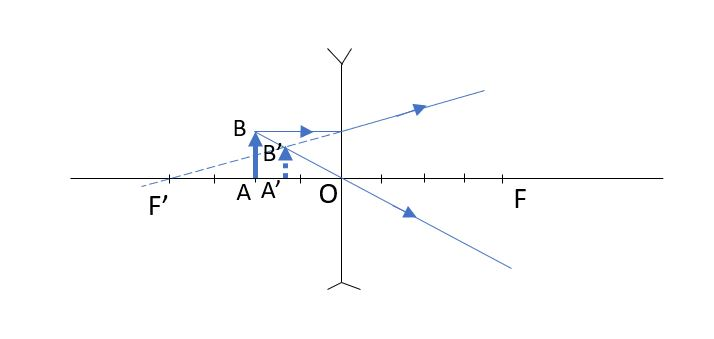
\includegraphics[scale=0.9]{../figs//VN11-2021-PH-TP032-06.JPG}
		\end{center}
	}
	\item \mkstar{2} [16]
	
	\cauhoi{
		
		Một thấu kính hội tụ có tiêu cự $\SI{40}{cm}$. Vật sáng AB cao $\SI{10}{cm}$ đặt vuông góc với trục chính của thấu kính và cách thấu kính $\SI{60}{cm}$. Hãy dựng ảnh của vật sáng AB qua thấu kính.
		
		
	}
	\loigiai{
		
	Vị trí của ảnh
		
		$$\dfrac{f} =\dfrac{1}{d} + \dfrac{1}{d'}  \Rightarrow d ' = \SI{120}{cm}.$$
		
		Độ phóng đại của thấu kính
		
		$$ k = - \dfrac{d}{d'} = -2.$$
		
		\begin{center}
			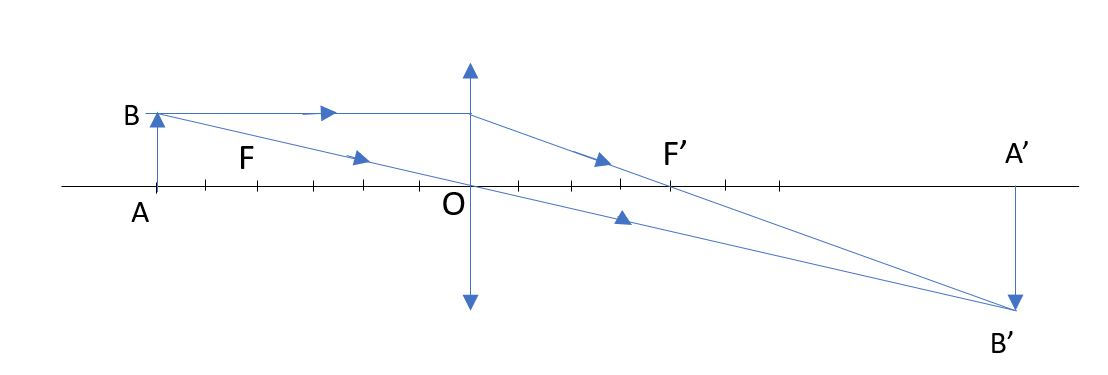
\includegraphics[scale=0.6]{../figs//VN11-2021-PH-TP032-07.JPG}
		\end{center}
	}
	\item \mkstar{2} [23]
	
	\cauhoi{
		
		Một thấu kính hội tụ có độ tụ $D = \SI{5}{dp}$. Đặt một vật sáng AB có chiều cao $\SI{2}{cm}$ trước thấu kính $\SI{40}{cm}$. Vẽ hình.
		
	}
	\loigiai{
		
		Tiêu cự của thấu kính
		
		$$f = \dfrac{1}{D} = \SI{20}{cm}.$$
		
		Vị trí của ảnh
		
		$$\dfrac{1}{d'} = \dfrac{1}{f} - \dfrac{1}{d} \Rightarrow d' = \SI{40}{cm}.$$
		
		Độ phóng đại của thấu kính
		
		$$ k =  - \dfrac{d'}{d} = -1.$$
		
		\begin{center}
			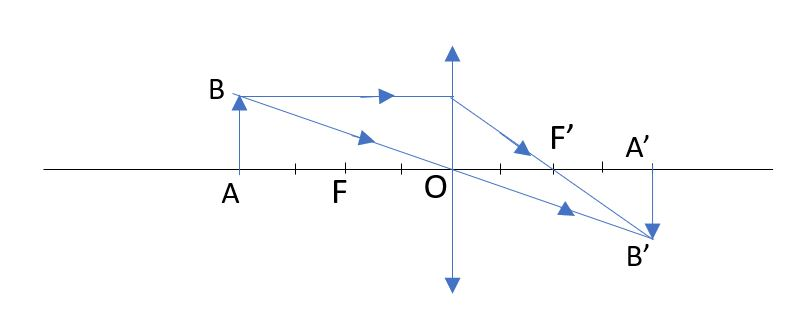
\includegraphics[scale=0.6]{../figs//VN11-2021-PH-TP032-08.JPG}
		\end{center}
	}

	\item \mkstar{2} [33]
	
	\cauhoi{
		
		Vật thật AB được đặt trên trục chính của thấu kính hội tụ có tiêu cự $\SI{20}{cm}$. Khoảng cách từ vật đến thấu kính là $\SI{30}{cm}$. Hãy xác định tính chất, chiều, độ lớn của ảnh, vẽ ảnh.
		
		
	}
	\loigiai{
		
		Vị trí ảnh
		
		$$\dfrac{1}{d'} = \dfrac{1}{f} - \dfrac{1}{d} \Rightarrow d' = \SI{60}{cm}.$$
		
		Độ phóng đại của thấu kính
		
		$$ k = - \dfrac{d'}{d} = -2 <0.$$
		
		Suy ra đây là ảnh thật, ngược chiều vật và cao gấp 2 lần vật.
		
		\begin{center}
			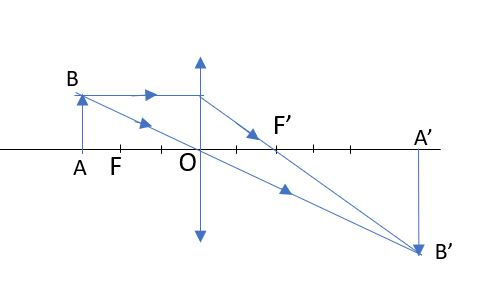
\includegraphics[scale=0.9]{../figs//VN11-2021-PH-TP032-09.JPG}
		\end{center}
	}

		\item \mkstar{2} [28]
	
	\cauhoi{
		
		
		\begin{enumerate}[label=\alph*)]
			\item Hình vẽ bên (Hình 1) biểu diễn loại thấu kính gì? Cho biết vì sao nó có tên gọi như vậy?
			\begin{center}
				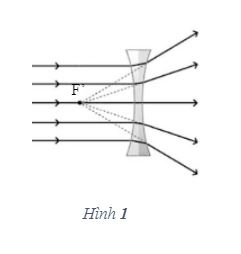
\includegraphics[scale=0.9]{../figs//VN11-2021-PH-TP028-13.JPG}
			\end{center}
			
			\item Cho khoảng cách từ quang tâm O đến một tiêu điểm chính của một thấu kính phân kỳ là $\SI{20}{cm}$. Đặt một vật sáng AB vuông góc với trục chính của thấu kính và cách thấu kính một đoạn $\SI{60}{cm}$. Xác định tiêu cự của thấu kính. Xác định vị trí, tính chất của ảnh và độ phóng đại. Vẽ hình (đúng tỉ lệ).
			\end{enumerate}
		
	}
	\loigiai{
		
		
		\begin{enumerate}[label=\alph*)]
			\item Thấu kính phân kì/thấu kính rìa dày/thấu kính lõm.
			
			Vì: nó làm phân kì chùm sáng tới song song/nó có phần rìa dày hơn phần giữa/nó có phần giữa lõm.
			
			\item Tiêu cự của thấu kính: $f = - \SI{20}{cm}.$
			
			Vị trí của ảnh: 
			
			$$d'=\dfrac{df}{d-f} =-\SI{15}{cm}.$$
			
			Tính chất của ảnh: ảnh ảo (do $d’ < 0$) 
			
			Độ phóng đại:
			
			$$k= - \dfrac{d'}{d} =\text{0,25}.$$ 
			
			
			\begin{center}
				\includegraphics[scale=0.9]{../figs//VN11-2021-PH-TP032-10.JPG}
			\end{center}
		\end{enumerate}
		
			
		
	}

	\item \mkstar{2} [10]
	
	\cauhoi{
		
		Một vật thật AB cao $\SI{10}{cm}$ đặt vuông góc trục chính của thấu kính có tiêu cự $f$ cho ảnh ảo A$_1$B$_1$ cao $\SI{20}{cm}$, ảnh cách thấu kính $\SI{10}{cm}$. Đây là thấu kính gì? Tiêu cự bằng bao nhiêu? Vẽ ảnh của vật qua thấu kính theo đúng tỉ lệ.
		
	}
	\loigiai{
		
			Ta có:
			
			$$ |k| = \dfrac{A_1B_1}{AB} = 2.$$
			
			Đây là thấu kính hội tụ do vật thật cho ảnh ảo lớn hơn vật, nên $ k>0$
			
			$$ k = - \dfrac{d'}{d}  \Rightarrow d = -\dfrac{d'}{k} = \SI{5}{cm} \ (d' = - \SI{10}{cm}).$$

			Tiêu cự của thấu kính 
			
			$$\dfrac{1}{f} = \dfrac{1}{d} + \dfrac{1}{d'} \Rightarrow f = \SI{10}{cm}.$$
			
			
			\begin{center}
				\includegraphics[scale=0.9]{../figs//VN11-2021-PH-TP032-11.JPG}
			\end{center}

}

\end{enumerate}

\section{Lý thuyết: Xác định vị trí, tính chất, độ lớn của vật và ảnh}
\begin{enumerate}[label=\bfseries Câu \arabic*:]
	
	\item \mkstar{1} [21]
	
	\cauhoi{
		Gọi $d$ là khoảng cách từ vật tới thấu kính, $d’$ là khoảng cách từ ảnh đến thấu kính và $f$ là tiêu cự của thấu kính. Độ phóng đại ảnh qua thấu kính là
		
		\begin{mcq}(2)
			\item $k = -\dfrac{d'}{d}.$
			\item $k = \dfrac{f}{f-d}.$
			\item $k = -\dfrac{f-d'}{f}.$
			\item Cả A, B, C đều đúng.
		\end{mcq}
		
		
	}
	\loigiai{
		
		\textbf{Đáp án: D.}
		
		Độ phóng đại ảnh qua thấu kính là $k = -\dfrac{d'}{d}.$
		
		Mà $$ \dfrac{1}{f} =\dfrac{1}{d} + \dfrac{1}{d'}.$$
	}
	\item \mkstar{1} [26]
	
	\cauhoi{
	Viết công thức liên hệ giữa tiêu cự, vị trí vật và vị trí ảnh. Cho biết quy ước về dấu của các đại lượng trong công thức.
	
	}
	\loigiai{
		
	* Công thức liên hệ giữa vị trí các vật và ảnh:  
	
	$$\dfrac{1}{f} = \dfrac{1}{d} +\dfrac{1}{d'}.$$
	
	* Quy ước: 
	
	 $f > 0$: thấu kính hội tụ; $f < 0$: thấu kính phân kì.
	
	 $d > 0$: Vật thật; $d < 0$: Vật ảo.
	
	 $d’ > 0$: ảnh thật; $d’ < 0$: Ảnh ảo.
	
	
	}
	\item \mkstar{2} [6]
	
	\cauhoi{
		
		Vật sáng AB đặt vuông góc với một trục chính của một thấu kính có tiêu cự $\SI{30}{cm}$ cho ảnh A’B’ = 3AB rõ nét trên màn. Xác định vị trí vật và ảnh. Vẽ ảnh minh họa.
		
	}
	\loigiai{
		
		Ta có:
		
		$$ |k| = \dfrac{\text{A'B'}}{\text{AB}} = 3.$$
		
		Mà ảnh hứng được trên màn là ảnh thật nên thấu kính này là thấu kính hội tụ, và ảnh thật ngược chiều vật và lớn hơn vật. $k < 0$
		
		$$ 3 = \left|-\dfrac{d'}{d}\right| \Rightarrow d' = 3d.$$
		
		Lại có:
		
		$$f = \dfrac{dd'}{d+d'} = 30.$$
		
		Suy ra $d = \SI{40}{cm}.$ và $d' = \SI{120}{cm}.$
		
		
		\begin{center}
			\includegraphics[scale=0.9]{../figs//VN11-2021-PH-TP032-12.JPG}
		\end{center}
		 
	}
	\item \mkstar{2} [7]
	
	\cauhoi{
		
		Một thấu kính hội tụ có tiêu cự $\SI{40}{cm}$. Vật sáng là đoạn thẳng AB đặt vuông góc với trục chính cách thấu kính $\SI{20}{cm}$. Xác định vị trí, tính chất ảnh A’B’ của AB.
		
		
	}
	\loigiai{
		
		+ Ta có: 
		
		$$d' = \dfrac{df}{d-f} = -\SI{40}{cm}.$$
		
		Do $d' <0$ nên đây là ảnh ảo.
		
		+ Độ phóng đại:
		
		$$ k = -\dfrac{d'}{d} = 2 > 0$$
		
		Ảnh cùng chiều với vật.
		
		$$|k| =2 >1 \Rightarrow \ \text{ảnh lớn hơn vật.}$$
		
	}
	\item \mkstar{2} [9]
	
	\cauhoi{
		
		Một vật sáng AB có chiều cao $\SI{1}{cm}$, đặt thẳng góc với trục chính của một thấu kính hội tụ có tiêu cự $\SI{20}{cm}$, cách thấu kính một khoảng $\SI{60}{cm}$ cho ảnh A’B’ (điểm A nằm trên trục chính). Xác định vị trí, chiều cao, độ phóng đại ảnh và tính chất của ảnh A’B’. Vẽ hình đúng tỉ lệ.
		
		
	}
	\loigiai{
		
		Ta có:
		
		$$\dfrac{1}{f} = \dfrac{1}{d} + \dfrac{1}{d'} \Rightarrow d' =\SI{30}{cm} > 0.$$
		
		Độ phóng đại
		
		$$ k  = - \dfrac{d'}{d} = -\dfrac{1}{2} = -\text{0,5}.$$
		
		Mà:
		
		$$|k| =\dfrac{\text{A'B'}}{\text{AB}} =\text{0,5} \Rightarrow \text{A'B'} =\text{0,5} \text{AB} = \SI{0,5}{cm}.$$
		
		 Tính chất ảnh: Ảnh thật (hứng được trên màn chắn), ngược chiều, nhỏ hơn vật.
		 
		 
		\begin{center}
			\includegraphics[scale=0.9]{../figs//VN11-2021-PH-TP028-22.JPG}
		\end{center}
				

	}
	\item \mkstar{2} [9]
	
	\cauhoi{
		Một vật sáng AB đặt thẳng góc với trục chính của một thấu kính phân kì có tiêu cự $f$, cách thấu kính một khoảng $\SI{60}{cm}$ cho ảnh A’B’ nhỏ hơn vật 4 lần. Xác định tiêu cự của thấu kính trên. Vẽ hình.
		
	}
	\loigiai{
		
		Đây là thấu kính phân kì nên ảnh là ảnh ảo.
		
		$$k > 0 \Rightarrow k = \dfrac{1}{4} = - \dfrac{d'}{d} \Rightarrow d' = - \SI{15}{cm}.$$
		
		Tiêu cự của thấu kính
		
		$$\dfrac{1}{f} =\dfrac{1}{d} + \dfrac{1}{d'} \Rightarrow f = -\SI{20}{cm}.$$
		
		\begin{center}
			\includegraphics[scale=0.9]{../figs//VN11-2021-PH-TP028-23.JPG}
		\end{center}
	}
		\item \mkstar{2} [13]
	
	\cauhoi{
		
		Cho xy là trục chính của thấu kính phân kỳ, AB là vật sáng, F và F' là các tiêu điểm chính. Hãy vẽ ảnh A'B' của vật AB cho bởi thấu kính. Ảnh A'B' là ảnh thật hay ảnh ảo và có độ lớn như thế nào so với vật AB?
		
		\begin{center}
			\includegraphics[scale=0.9]{../figs//VN11-2021-PH-TP032-03.JPG}
		\end{center}
	}
	\loigiai{
		
		Thấu kính phân kỳ cho ảnh ảo, cùng chiều và bé hơn vật.
		
		
		\begin{center}
			\includegraphics[scale=0.9]{../figs//VN11-2021-PH-TP032-13.JPG}
		\end{center}
	}
	\item \mkstar{2} [24]
	
	\cauhoi{
		Vật sáng AB  được đặt vuông góc với trục chính của một thấu kính hội tụ có tiêu cự $\SI{20}{cm}$ và cách thấu kính $\SI{60}{cm}$. Xác định vị trí, tính chất, chiều và độ lớn của ảnh A$_1$B$_1$ qua thấu kính. Vẽ hình.
		
	}
	\loigiai{
		
		Vị trí của ảnh
		
		$$d'= \dfrac{df}{d-f}=\SI{30}{cm} >0.$$
		
		Suy ra ảnh là ảnh thật, ngược chiều.
		
		Độ phóng đại
		
		$$ k =-\dfrac{d'}{d} = - \dfrac{1}{2}.$$
		
		Ảnh có độ lớn bằng một nửa vật.
		
		\begin{center}
			\includegraphics[scale=0.9]{../figs//VN11-2021-PH-TP032-14.JPG}
		\end{center}
	}
	\item \mkstar{2} [25]
	
	\cauhoi{
		
		Vật sáng AB bằng $\SI{2}{cm}$ đặt vuông góc với trục chính của thấu kính hội tụ có tiêu cự $f = \SI{40}{cm}$, cách thấu kính một khoảng $\SI{50}{cm}$. Xác định vị trí, tính chất và độ lớn ảnh A’B’ của AB qua thấu kính. Vẽ hình.
		
		
	}
	\loigiai{
		
		Ta có: 
		
		$$d' = \dfrac{df}{d-f} = \SI{200}{cm.}$$
		
		Độ phóng đại 
		
		$$k = - \dfrac{d'}{d} =-4.$$
		
		Ảnh là ảnh thật, ngược chiều vật, cao gấp 4 lần vật.
		
		\begin{center}
			\includegraphics[scale=0.6]{../figs//VN11-2021-PH-TP032-15.JPG}
		\end{center}
	}
	
	
	
	
	\item \mkstar{2} [26]
	
	\cauhoi{
		Vật sáng AB đặt vuông góc với trục chính của một thấu kính hội tụ, cách thấu kính $\SI{12}{cm}$, cho ảnh ảo A$_1$B$_1$. Ảnh này cao gấp 2 lần vật. Xác định tiêu cự của thấu kính.
		
		
	}
	\loigiai{
		
		Ta có:
		
		$$ |k| = \left| - \dfrac{d'}{d}\right| = \dfrac{A_1B_1}{AB} =2.$$
		
		Mà vật thật, ảnh ảo
		
		$$ k = - \dfrac{d'}{d} = 2 \Rightarrow d' =-2d = -\SI{24}{cm}.$$
		
		Tiêu cự của thấu kính
		
		$$\dfrac{1}{f} = \dfrac{1}{d} + \dfrac{1}{d'} \Rightarrow f =\SI{24}{cm}.$$
	}
	\item \mkstar{3} [37]
	
	\cauhoi{
		
		Cho thấu kính hội tụ có tiêu cự $\SI{20}{cm}$. Vật sáng AB là một đoạn thẳng cao $\SI{2}{cm}$ đặt vuông góc trục chính của thấu kính, cách thấu kính $\SI{30}{cm}$. 
		
		\begin{enumerate}[label=\alph*)]
			\item Hãy tính độ tụ của thấu kính trên.
			\item Hãy xác định vị trí ảnh, tính chất ảnh, số phóng đại ảnh và độ cao ảnh. Vẽ hình đúng tỷ lệ.  
			\item Thay thấu kính trên bằng một thấu kính khác sao cho khi  AB cách thấu kính một đoạn $\SI{10}{cm}$ ta thu được ảnh ảo cao $\SI{6}{cm}$. Đây là thấu kính loại gì? Tại sao? Có tiêu cự bằng bao nhiêu?   
		\end{enumerate}
	}
	\loigiai{
		
		\begin{enumerate}[label=\alph*)]
			\item Độ tụ của thấu kính
			
			$$D = \dfrac{1}{f} = \SI{5}{dp}.$$
			
			\item Ta có:
			
			$$\dfrac{1}{f}=\dfrac{1}{d} + \dfrac{1}{d'} \Rightarrow d' = \SI{60}{cm} > 0.$$
			
			Suy ra ảnh là ảnh thật.
			
			Lại có:
			
			$$k = - \dfrac{d'}{d} = -2.$$
			
			Suy ra: 
			
			$$\text{A'B'} = |k| \text{AB} = \SI{4}{cm}.$$
			
			\begin{center}
				\includegraphics[scale=0.8]{../figs//VN11-2021-PH-TP032-16.JPG}
			\end{center}
			
			\item Vì ảnh ảo cao hơn vật nên đây là thấu kính hội tụ $\text{AB} = \SI{2}{cm}$ và $\text{A'B'} = \SI{6}{cm}.$
			
			Suy ra:
			
			$$ k = 3 = - \dfrac{d'}{d} = \dfrac{f}{d-f}.$$
			
			Giải phương trên ta có $$f= \SI{15}{cm}.$$
			
		\end{enumerate}      
	}
	\item \mkstar{3} [36]
	
	\cauhoi{
		
		Một thấu kính hội tụ có tiêu cự $\SI{6}{cm}$. Vật sáng AB cao $\SI{2}{cm}$ đặt vuông góc với trục chính của thấu kính và cách thấu kính $\SI{8}{cm}$.
		
		\begin{enumerate}[label=\alph*)]
			\item Hãy xác định vị trí, tính chất và độ cao ảnh A’B’ của AB qua thấu kính?
			\item Giữ nguyên vật AB, vị trí của vật và thấu kính. Để thu được ảnh ảo cao gấp 3 lần vật thì ta phải thay thấu kính trên bằng một thấu kính có tiêu cự bằng bao nhiêu ?
		\end{enumerate} 

	}
	\loigiai{
		
	\begin{enumerate}[label=\alph*)]
		\item Ta có: 
		
		$$\dfrac{1}{f} = \dfrac{1}{d} + \dfrac{1}{d'} \Rightarrow d' = \SI{24}{cm} >0 \Rightarrow \text{ảnh thật}.$$
		
		Độ phóng đại
		
		$$ k = - \dfrac{d'}{d} = -3.$$
		
		Mà 
		
		$$|k| = \dfrac{\text{A'B'}}{\text{AB}} \Rightarrow \text{A'B'} = \SI{6}{cm}.$$
		
		Vậy ảnh thu được là ảnh thật, cao $\SI{6}{cm}$ và cách thấu kính $\SI{24}{cm}.$
	
		\item Ta có: 
		
		$$|k_1| = \dfrac{\text{A'B'}}{\text{AB}} =3.$$
		
		Vậy $k_1 =3 \Rightarrow 3 = - \dfrac{d'}{d} \Rightarrow d' = -\SI{24}{cm}.$
		
		Mà
		
		$$\dfrac{1}{f_1} = \dfrac{1}{d} + \dfrac{1}{d'} \Rightarrow f_1 =\SI{12}{cm}.$$ 
	
	\end{enumerate}
	}
	\item \mkstar{3} [35]
	
	\cauhoi{
		 Một vật sáng AB hình mũi tên cao $\SI{2}{cm}$ đặt vuông góc với trục chính của thấu kính (A trên trục chính) cách thấu kính một đoạn $d$.
		 \begin{enumerate}[label=\alph*)]
		 	\item Khi vật AB cách thấu kính một đoạn $d = \SI{15}{cm}$, qua thấu kính cho 1 ảnh thật cao $\SI{4}{cm}$. Xác định loại thấu kính. Tính tiêu cự và độ tụ của thấu kính. Vẽ hình minh họa. 
		 	\item Từ vị trí vật ở câu a, dịch chuyển vật dọc theo trục chính của thấu kính một đoạn thì thu được một ảnh ảo, cao gấp 2 lần vật. Hãy xác định vị trí mới của vật và ảnh. 
		 \end{enumerate}
		
		
	}
	\loigiai{
		\begin{enumerate}[label=\alph*)]
			\item Thấu kính hội tụ: Vì vật thật cho ảnh thật, ảnh lớn hơn vật nên ảnh sẽ ngược chiều vật.
			
			$$k = \dfrac{\text{A'B'}}{\text{AB}} = - 2 = -\dfrac{d'}{d} \Rightarrow   d' =2d =\SI{30}{cm}.$$
			
			Tiêu cự của thấu kính
			
			$$f = \dfrac{d'd}{d+d'} = \SI{10}{cm}.$$
			
			Độ tụ của thấu kính
			
			$$D = \dfrac{1}{f} = \SI{10}{dp}.$$
			
			\begin{center}
				\includegraphics[scale=0.9]{../figs//VN11-2021-PH-TP032-01.JPG}
			\end{center}
			\item Ảnh cùng chiều với vật thật là ảnh ảo: $k = 2$.
			
			Ta có:
			
			$$k = 2 = - \dfrac{d'}{d}\ (1).$$
			
			Và:
			
			$$\dfrac{1}{f} = \dfrac{1}{d} + \dfrac{1}{d'}\ (2).$$
			
			Vị trí vật:
			
			$$\dfrac{1}{f} = \dfrac{1}{d} - \dfrac{1}{2d} = \dfrac{1}{2d} \Rightarrow d = \SI{5}{cm}.$$
			
			Vị trí ảnh: 
			
			$$d' = -2d = -\SI{10}{cm}.$$
			
		\end{enumerate}
		 
	}
	\item \mkstar{3} [34]
	
	\cauhoi{
		
		Một thấu kính phân kỳ có tiêu cự $-\SI{40}{cm}$. Vật sáng $\text{AB} = \SI{2,4}{cm}$ đặt vuông góc trục chính và cách thấu kính một đoạn $\SI{20}{cm}$. Xác định vị trí, tính chất, chiều và độ lớn ảnh và vẽ ảnh.
		
		
	}
	\loigiai{
		
		Vị trí ảnh 
		
		$$ \dfrac{1}{d'} = \dfrac{1}{f} - \dfrac{1}{d} \Rightarrow d = -\dfrac{40}{3}.$$.
		
		Độ phóng đại của thấu kính
		
		$$ k  = -\dfrac{d'}{d} = \dfrac{2}{3}.$$
		
		Do thấu kính phân kỳ nên ảnh là ảnh ảo, cùng chiều và bằng  $\dfrac{2}{3}$ vật.
		
		\begin{center}
			\includegraphics[scale=0.9]{../figs//VN11-2021-PH-TP032-17.JPG}
		\end{center}
	}
	\item \mkstar{3} [11]
	
	\cauhoi{
		
		Một thấu kính hội tụ có độ tụ $\SI{2}{dp}$. 
		\begin{enumerate}[label=\alph*)]
			\item Tính tiêu cự của thấu kính. 
			\item Một vật thật AB cao $\SI{6}{cm}$ đặt vuông góc với trục chính của thấu kính, cách thấu kính $\SI{20}{cm}$. Xác định vị trí, tính chất và chiều cao của ảnh tạo bởi thấu kính.
		\end{enumerate}
		
	}
	\loigiai{
		
			\begin{enumerate}[label=\alph*)]
				
			\item Tiêu cự của thấu kính
			
			$$f=\dfrac{1}{D} = \SI{0,5}{m} = \SI{50}{cm}.$$
			
			\item Khoảng cách từ ảnh đến quang tâm
			
			$$d'=\dfrac{df}{d-f}= -\dfrac{100}{3}\ \text{cm}.$$
			
			A’B’ là ảnh ảo cách thấu kính $\dfrac{100}{3}\ \text{cm}.$
			
			Số phóng đại ảnh: $$k=-\dfrac{d'}{d}=\dfrac{5}{3}.$$
			
			Chiều cao ảnh là $$\text{A’B’} = |k| \text{AB} = \SI{10}{cm}.$$
			
			\end{enumerate}
		
	}
	\item \mkstar{3} [12]
	
	\cauhoi{
		
		Vật sáng AB có điểm A nằm trên trục chính và vuông góc với trục chính của một thấu kính hội tụ. Vật AB cách thấu kính $\SI{40}{cm}$ ta thu được ảnh thật cao bằng nửa vật.
		\begin{enumerate}[label=\alph*)]
			\item Xác định vị trí ảnh và tiêu cự của thấu kính. 
			
			\item Vẽ ảnh A’B’ thu được qua thấu kính.
		\end{enumerate}
		
	}
	\loigiai{
		
		\begin{enumerate}[label=\alph*)]
			\item Vì ảnh thật (ngược chiều) bằng nửa vật nên $k < 0$
			
			$$\Rightarrow   k = - \text{0,5}.$$  
			
			Ta có:
			
			$$k = -\dfrac{d'}{d} \Rightarrow d’= \SI{20}{cm}.$$
			
			Tiêu cực của thấu kính
			
			$$\dfrac{1}{f} = \dfrac{1}{d} + \dfrac{1}{d'} \Rightarrow f =\dfrac{40}{3}\ \text{cm} = \SI{13,33}{cm}.$$
			
			\item Hình vẽ
			
			\begin{center}
				\includegraphics[scale=0.9]{../figs//VN11-2021-PH-TP032-02.JPG}
			\end{center}
		\end{enumerate}
	}

	\item \mkstar{3} [14]
	
	\cauhoi{
		
		Vật sáng AB cao $\SI{4}{cm}$ đặt vuông góc với trục chính của một thấu kính hội tụ có tiêu cự $\SI{20}{cm}$ và cách thấu kính $\SI{10}{cm}$.
		\begin{enumerate}[label=\alph*)]
			\item Tìm khoảng cách từ ảnh tới thấu kính. Tính số phóng đại ảnh và độ cao của ảnh.
			
			\item  Nêu tính chất ảnh. Vẽ hình đúng tỉ lệ.
		\end{enumerate}
		
	}
	\loigiai{
		
		\begin{enumerate}[label=\alph*)]
			\item Vị trí ảnh:
			
			$$d' = \dfrac{df}{d-f} =-\SI{20}{cm}.$$
			
			Hệ số phóng đại:
			
			$$ k = - \dfrac{d'}{d} = 2.$$
			
			Độ cao ảnh
			
			$$\text{A'B'} =|k| \text{AB} = \SI{4}{cm}.$$
			\item 
			Thấu kính hội tụ có $d < f$ nên cho ảnh ảo, cùng chiều và lớn hơn vật.
			\begin{center}
				\includegraphics[scale=0.9]{../figs//VN11-2021-PH-TP032-18.JPG}
			\end{center}
		\end{enumerate}
	}

	\item \mkstar{3} [16]
	
	\cauhoi{
		
		 Một thấu kính hội tụ có tiêu cự $\SI{40}{cm}$. Vật sáng AB cao $\SI{10}{cm}$ đặt vuông góc với trục chính của thấu kính và cách thấu kính $\SI{60}{cm}$. Hãy:
	\begin{enumerate}[label=\alph*)]
		\item Xác định vị trí, tính chất, độ cao của ảnh qua thấu kính.
		\item Dựng ảnh của vật sáng AB qua thấu kính.
	\end{enumerate}
		
	}
	\loigiai{
		
		\begin{enumerate}[label=\alph*)]
			\item Xác định vị trí, tính chất, độ cao của ảnh qua thấu kính:
			
			- Vị trí ảnh:
			
			$$\dfrac{1}{f} = \dfrac{1}{d} + \dfrac{1}{d'} \Rightarrow d' = \SI{120}{cm}.$$
			
			- Độ phóng đại:
			
			$$ k =-\dfrac{d'}{d} = -2 <0.$$
			
			Suy ra đây là ảnh thật, ngược chiều.
			
			- Độ cao ảnh
			
			$$\text{A'B'} = |k| \text{AB} = \SI{20}{cm}.$$
			
			
			\item Dựng ảnh của vật sáng qua thấu kính hội tụ:
			
			\begin{center}
				\includegraphics[scale=0.9]{../figs//VN11-2021-PH-TP032-04.JPG}
			\end{center}
		\end{enumerate}
	}
	\item \mkstar{3} [16]
	
	\cauhoi{
		
		 Đặt một vật sáng AB trước một thấu kính có tiêu cự $|f| = \SI{60}{cm}$ và vuông góc với trục chính. Cho biết khoảng cách từ ảnh đến thấu kính là $-\SI{30}{cm}$. Gọi $\overline{A_1B_1}$ là độ cao của ảnh cho bởi thấu kính hội tụ, $\overline{A_2B_2}$ là độ cao của ảnh cho bởi thấu kính phân kỳ. Hãy xác định tỉ số $\dfrac{\overline{A_2B_2}}{\overline{A_1B_1}}$.
		
		
	}
	\loigiai{
		
		* Ảnh tạo bởi thấu kính hội tụ: ($f > 0, f = \SI{60}{cm}$).
		
		Ta có:
		
		$$\dfrac{1}{f} =\dfrac{1}{d} + \dfrac{1}{d'} \Rightarrow d = \SI{20}{cm}.$$
		
		Số phóng đại:
		
		$$k = -\dfrac{d'}{d} = \dfrac{3}{2},$$
		
		Vậy:
		
		$$\overline{A_1B_1} =|k| \overline{AB} = \dfrac{3}{2}\overline{AB}.$$
		
		* Ảnh tạo bởi thấu kính phân kỳ: ($f < 0, f = -\SI{60}{cm}$)
		
		Ta có:
		
		$$\dfrac{1}{f} =\dfrac{1}{d} + \dfrac{1}{d'} \Rightarrow d = \SI{60}{cm}.$$
		
		Số phóng đại:
		
		$$k = -\dfrac{d'}{d} = \dfrac{1}{2},$$
		
		Vậy: $$\overline{A_2B_2} =|k| \overline{AB} = \dfrac{1}{2}\overline{AB}.$$
		
		Tỉ số: $\dfrac{\overline{A_2B_2}}{\overline{A_1B_1}} = \dfrac{1}{3}.$
	}
	\item \mkstar{3} [17]
	
	\cauhoi{
		Một vật sáng AB cao $\SI{3}{cm}$ nằm vuông góc với trục chính của một thấu kính hội tụ và cách thấu kính một khoảng $\SI{60}{cm}$. Tiêu cự của thấu kính là $\SI{20}{cm}$.
		\begin{enumerate}[label=\alph*)]
			\item Tính độ tụ thấu kính.
			\item Tính khoảng cách từ ảnh đến vật. 
			\item Tính độ phóng đại $k$ và cho biết tính chất của ảnh.
			\item Tìm chiều cao của ảnh A’B’.
			\item Vẽ hình đúng tỉ lệ.
		\end{enumerate}
		
	}
	\loigiai{
		
		\begin{enumerate}[label=\alph*)]
			\item Độ tụ của thấu kính
			
			$$D=\dfrac{1}{f}=\SI{5}{dp}.$$
			
			\item Khoảng cách từ ảnh đến vật 
			
			$$d'=\dfrac{df}{d-f} = \SI{30}{cm}.$$
			
			\item Độ phóng đại $k$
			
			$$k=-\dfrac{d'}{d} = - \text{0,5}.$$
			
			Suy ra ảnh thật, ngược chiều.
			\item Chiều cao của ảnh A'B'
			
			$$\text{A'B'}=|k| \text{AB} = \SI{1,5}{cm}.$$
			\item Hình vẽ
			
			\begin{center}
				\includegraphics[scale=0.9]{../figs//VN11-2021-PH-TP032-19.JPG}
			\end{center}
		\end{enumerate}
	}
	\item \mkstar{3} [18]
	
	\cauhoi{
		Một vật nhỏ, phẳng AB được đặt trên trục chính và vuông góc với trục chính của một thấu kính hội tụ có tiêu cự $\SI{20}{cm}$. Vật AB đặt cách thấu kính $\SI{30}{cm}$. 
		\begin{enumerate}[label=\alph*)]
			\item Xác định vị trí ảnh, tính chất của ảnh.
			\item Tìm số phóng đại của ảnh. So sánh chiều và độ lớn của ảnh so với vật. Vẽ ảnh.
		\end{enumerate}
		
	}
	\loigiai{
		
		Cho $f = \SI{20}{cm}, d= \SI{30}{cm}.$
		
		\begin{enumerate}[label=\alph*)]
			\item Vị trí ảnh,tính chất của ảnh
			
			$$\dfrac{1}{f} = \dfrac{1}{d} + \dfrac{1}{d'} \Rightarrow d' = \SI{60}{cm} >0.$$
			
			Ảnh A’B’ thật cách thấu kính $\SI{60}{cm}$.
		
			\item Số phóng đại $$k=-\dfrac{d’}{d} = -2. $$
			
			Ảnh A’B’ ngược chiều, lớn gấp 2 lần vật cách thấu kính $\SI{60}{cm}$.
			
			 
			\begin{center}
				\includegraphics[scale=0.9]{../figs//VN11-2021-PH-TP032-20.JPG}
			\end{center}
			
		\end{enumerate}
	}
	\item \mkstar{3} [19]
	
	\cauhoi{
		Một thấu kính có độ tụ $\SI{2}{dp}$. Vật sáng AB đặt vuông góc với trục chính thấu kính (A nằm trên trục chính) cách thấu kính $\SI{60}{cm}$.
		\begin{enumerate}[label=\alph*)]
			\item Tính tiêu cự của thấu kính.
			\item Tính khoảng cách từ ảnh của AB đến thấu kính. Ảnh là ảnh thật hay ảnh ảo và cao gấp mấy lần vật AB. 
		\end{enumerate}
	}
	\loigiai{
		
		\begin{enumerate}[label=\alph*)]
			\item Tiêu cự của thấu kính
			
			$$f = \dfrac{1}{D} = \SI{0,5}{m}.$$
			
			\item Khoảng cách từ ảnh của AB đến thấu kính
			
			$$d' = \dfrac{df}{d-f} = \SI{3}{m}.$$
			
			$$ k= - \dfrac{d'}{d} = -5< 0.$$ 
			
			Ảnh là ảnh thật và cao gấp 5 lần vật.
		\end{enumerate}
	}
	\item \mkstar{3} [20]
	
	\cauhoi{
		
		Thấu kính hội tụ có độ tụ là $\SI{5}{dp}$.
	\begin{enumerate}[label=\alph*)]
		\item Tìm tiêu cự của thấu kính.
		\item Vật thật đặt trước thấu kính (vuông góc với trục chính của thấu kính) cho ảnh thật bằng 2 lần vật. Hãy xác định vị trí vật và vị trí ảnh. Vẽ hình đúng tỷ lệ. 
	\end{enumerate}
		
	}
	\loigiai{
		
		\begin{enumerate}[label=\alph*)]
			\item Tiêu cự của thấu kính
			
			$$f = \dfrac{1}{D} = \SI{20}{cm}.$$
			
			\item Độ phóng đại
			
			$$ k = - \dfrac{d'}{d} =-2 \Rightarrow d' = -2d.$$
			
			Thế vào công thức 
			
			$$\dfrac{1}{f} = \dfrac{1}{d} +\dfrac{1}{d'} \Rightarrow d = \SI{30}{cm}.$$
			
			$$\Rightarrow d' = \SI{60}{cm}.$$
			
			\begin{center}
				\includegraphics[scale=0.9]{../figs//VN11-2021-PH-TP032-20.JPG}
			\end{center}
		\end{enumerate}
	}

	\item \mkstar{3} [21]
	
	\cauhoi{
		Một vật sáng AB cao $\SI{1}{cm}$ được đặt vuông góc với trục chính của một thấu kính hội tụ cho một ảnh thật A$_1$B$_1$ hiện rõ nét trên màn đặt cách thấu kính $\SI{60}{cm}$ và ảnh này cao $\SI{3}{cm}$. Tìm tiêu cự.
	}
	\loigiai{
		
		Thấu kính hội tụ cho ảnh thật, ngược chiều vật.
		
		Độ phóng đại của thấu kính
		
		$$ k = - \dfrac{d'}{d} = - 3.$$
		
		Vị trí của ảnh
		
		$$ d + d' = \SI{60}{cm}.$$
		
		Suy ra: $d = \SI{15}{cm}$; $d' = \SI{45}{cm}.$
		
		Tiêu cự của thấu kính
		
		$$\dfrac{1}{f} = \dfrac{1}{d} + \dfrac{1}{d'} \Rightarrow f = \SI{11,25}{cm}. $$
		
	}

		\item \mkstar{3} [22]
	
	\cauhoi{
		
		Vật sáng AB cao $\SI{2}{cm}$ đặt vuông góc với trục chính của một thấu kính hội tụ có tiêu cự $\SI{36}{cm}$, vật cách thấu kính $\SI{60}{cm}$. Xác định vị trí, độ phóng đại, chiều cao ảnh A$_1$B$_1$ của vật AB cho bởi thấu kính. 
	}
	\loigiai{
		
		Vị trí ảnh
		
		$$d'  = \dfrac{df}{d-f} = \SI{90}{cm}.$$
		
		Độ phóng đại 
		
		$$ k = - \dfrac{d'}{d} = -\text{1,5}.$$
		
		Chiều cao của ảnh A$_1$B$_1$
		
		$$ A_1B_1 = |k| AB =\SI{3}{cm}.$$
		
		
	}
	\item \mkstar{3} [23]
	
	\cauhoi{
		Một thấu kính hội tụ có độ tụ $D = \SI{5}{dp}$. Đặt một vật sáng AB có chiều cao $\SI{2}{cm}$ trước thấu kính $\SI{40}{cm}$.
		
		\begin{enumerate}[label=\alph*)]
			\item Xác định tiêu cự của thấu kính.
			\item Xác định vị trí, độ phóng đại, độ cao của ảnh.
		\end{enumerate}
	}
	\loigiai{
		
		\begin{enumerate}[label=\alph*)]
			\item Tiêu cự của thấu kính
			
			$$ f=\dfrac{1}{D} = \SI{20}{cm}.$$
			
			\item Vị trí của vật
			
			$$\dfrac{1}{f} = \dfrac{1}{d} + \dfrac{1}{d'} \Rightarrow d' = \SI{40}{cm}.$$
			
			Độ phóng đại 
			
			$$ k  = -\dfrac{d'}{d} =-1.$$
			
			Chiều cao của ảnh
			
			$$\text{A'B'} = |k|\text{AB} =\SI{2}{cm}.$$
			
			
		\end{enumerate}
		
	}
	
	
	\item \mkstar{3} [27]
	
	\cauhoi{
		Cho một vật sáng AB cao $\SI{2}{cm}$ đặt vuông góc với trục chính của một thấu kính hội tụ có tiêu cự $\SI{25}{cm}$. 
		
		\begin{enumerate}[label=\alph*)]
			\item Tính độ tụ của thấu kính.
			\item Biết vật AB đặt cách thấu kính $\SI{15}{cm}$. Xác định vị trí, tính chất và chiều cao ảnh. 
		\end{enumerate}
		
	}
	\loigiai{
		
		\begin{enumerate}[label=\alph*)]
			\item Độ tụ của thấu kính
			
			$$ D = \dfrac{1}{f} = \SI{4}{dp}.$$
			\item Ta có:
			
			$$\dfrac{1}{f} = \dfrac{1}{d} + \dfrac{1}{d'} \Rightarrow d' =-\SI{37,7}{cm}.$$
			
			Độ phóng đại của thấu kính
			
			$$ k = - \dfrac{d'}{d} = -\text{2,5}.$$
			
			Chiều cao của ảnh
			
			$$\text{A'B'} = |k|AB = \SI{5}{cm}.$$
			
			
		\end{enumerate}
	}
\end{enumerate}	
\section{Lý thuyết: Dời vật hoặc thấu kính}
\begin{enumerate}[label=\bfseries Câu \arabic*:]
		\item \mkstar{3} [6]
	
	\cauhoi{
		Vật sáng AB đặt vuông góc với trục chính của một thấu kính có tiêu cự $\SI{30}{cm}$ cho ảnh A’B’ = 3AB rõ nét trên màn. Để thu được ảnh A’B’ = 0,5AB trên  màn  ta phải di chuyển vật sáng  đến gần hay ra xa một đoạn là bao nhiêu?
	}
	\loigiai{
		
		Cho ảnh thật $k= -3$
		
		$$k =-\dfrac{d'}{d}= -3 \Rightarrow d'=3d.$$
		
		Lại có:
		
		$$\dfrac{1}{f} = \dfrac{1}{d}+ \dfrac{1}{d'} \Rightarrow d = \SI{40}{cm}; d' =\SI{120}{cm}.$$
		
		Do ảnh thật nên 
		
		$$ k_1 =-\text{-0,5} = \dfrac{f}{f - d_1} \Rightarrow d_1 = \SI{90}{cm}.$$
		
		Do $d_1 >d$ nên vật di chuyển ra xa một đoạn $\Delta d = 90 -40=\SI{50}{cm}.$
	}
	
		\item \mkstar{3} [21]
	
	\cauhoi{
		Một vật sáng AB cao $\SI{1}{cm}$ được đặt vuông góc với trục chính của một thấu kính hội tụ cho một ảnh thật A$_1$B$_1$ hiện rõ nét trên màn đặt cách thấu kính $\SI{60}{cm}$ và ảnh này cao $\SI{3}{cm}$. Giữ nguyên thấu kính, muốn quan sát được ảnh A$_2$B$_2$ cùng chiều và cách vật AB một đoạn $\SI{20}{cm}$ thì phải dời vật một đoạn bao nhiêu theo chiều nào?   
	}
	\loigiai{
		
		Độ phóng đại của thấu kính
		
		$$ k  =  - \dfrac{d'}{d} = -3.$$
		
		Ta có:
		
		$$d + d' = \SI{60}{cm}.$$
		
		Suy ra $d = \SI{15}{cm}$; $d' = \SI{45}{cm}.$
		
		Tiêu cực của thấu kính
		
		$$f = \dfrac{dd'}{d + d'} = \dfrac{45}{4}\ \text{cm}.$$
		
		Qua thấu kính hội tụ muốn cho ảnh cùng chiều thì là ảnh ảo.
		
		$$ d'_1 - d_1 = \SI{20}{cm}.$$
		
		Lại có:
		
		$$\dfrac{1}{f} = \dfrac{1}{d_1} + \dfrac{1}{d'_1} = \dfrac{4}{45}.$$
		
		Suy ra $d_1=\SI{8}{cm}.$
		
	}
		\item \mkstar{3} [21]
	
	\cauhoi{
		Vật sáng AB  đặt trên trục chính, vuông góc với trục chính của một thấu kính, cho ảnh thật A’B’ rõ nét trên màn.Giữ cố định thấu kính, khi dời vật ra xa thấu kính một đoạn $\SI{2}{cm}$ dọc theo trục chính, và dời màn một đoạn $\SI{30}{cm}$ thì thu được  ảnh rõ  nét trên màn  nhưng ảnh này bằng 0,6  lần ảnh trước. Tìm tiêu cự của thấu kính.
		
		
	}
	\loigiai{
		
		Áp dụng công thức 
		
		$$\dfrac{1}{f}=  \dfrac{1}{d}+\dfrac{1}{d’}$$
		
		$$k=\dfrac{f}{f-d}$$
		
		$$k= \dfrac{f-d’}{f}$$   
		
		Suy ra $f= \SI{15}{cm}.$
	}
		\item \mkstar{3} [22]
	
	\cauhoi{

		Vật sáng AB cao $\SI{2}{cm}$ đặt vuông góc với trục chính của một thấu kính hội tụ có tiêu cự $\SI{36}{cm}$, vật cách thấu kính $\SI{60}{cm}$. Giữ nguyên vị trí thấu kính, dịch  chuyển vật AB sao cho ảnh mới A$_2$B$_2$ cao bằng ảnh A$_1$B$_1$. Hỏi dịch chuyển vật lại gần hay ra xa thấu kính một đoạn bao nhiêu? 
		
	}
	\loigiai{
		
		Vị trí ảnh
		
		$$d'  = \dfrac{df}{d-f} = \SI{90}{cm}.$$
		
		Độ phóng đại 
		
		$$ k = - \dfrac{d'}{d} = -\text{1,5}.$$
		
		Chiều cao của ảnh A$_1$B$_1$
		
		$$ A_1B_1 = |k| AB =\SI{3}{cm}.$$
		
		Ảnh mới A$_2$B$_2$ cao bằng ảnh A$_1$B$_1$. Suy ra ảnh mới A$_2$B$_2$ chỉ là ảnh ảo.
		
		$$k =\text{1,5} = - \dfrac{f}{d_2 - f} \Rightarrow d_2 = \SI{12}{cm}.$$
		
		Dời vật lại gần thấu kính 48 cm.
		
		
	}
		\item \mkstar{3} [24]
	
	\cauhoi{
		Vật sáng AB  được đặt vuông góc với trục chính của một thấu kính hội tụ có tiêu cự $\SI{20}{cm}$ và cách thấu kính $\SI{60}{cm}$. Thay đổi vị trí của vật sáng AB ta có một ảnh khác là A$_2$B$_2$ bằng 0,6 lần vật. Xác định vị trí của vật lúc này.
		
	}
	\loigiai{
		
		Vị trí ảnh
		
		$$\dfrac{1}{d} = \dfrac{1}{f} - \dfrac{1}{d'} \Rightarrow d = \SI{30}{cm}.$$
		
		Độ phóng đại lúc đầu
		
		$$ k = - \dfrac{d'}{d} = - \text{0,5}. \ (1)$$
		
		Độ phóng đại lúc sau
		
		$$k_1 = \dfrac{d'}{d_1} = - \text{0,6}. \ (2)$$
		
		Lấy (1)  chia (2):
		
		$$\dfrac{d_1}{d} = \dfrac{5}{6} \Rightarrow d_1 = \SI{50}{cm}.$$
	}
		\item \mkstar{3} [24]
	
	\cauhoi{
		
	Một vật sáng phẳng AB được đặt trước một thấu kính, vuông góc với trục chính. Ảnh A$_1$B$_1$ của vật tạo bởi thấu kính bằng sáu lần vật. Dời vật lại gần thấu kính một đoạn $\SI{15}{cm}$. Ảnh của vật A$_2$B$_2$ ở vị trí mới vẫn bằng sáu lần vật. Tính tiêu cự của thấu kính.
	
		
	}
	\loigiai{
		
		Từ đề bài suy ra $ k_1 =-6$; $k_2 =6.$
		
		$$k = - \dfrac{f}{d-f} \Rightarrow d =f - \dfrac{f}{k}.$$
		
		$$d_1 =f - \dfrac{f}{k_1}\ (1).$$
		
		$$d_2 = f - \dfrac{f}{k_2}\ (2).$$
		
		$$d_1-d_2 =15\ (3).$$
		
		Kết hợp 1, 2, 3 giải ra $f =\SI{15}{cm}.$
	}
		\item \mkstar{3} [25]
	
	\cauhoi{
		
	Vật sáng AB bằng $\SI{2}{cm}$ đặt vuông góc với trục chính của thấu kính hội tụ có tiêu cự $f = \SI{40}{cm}$, cách thấu kính một khoảng $\SI{50}{cm}$. Để thấu kính cố định, phải tịnh tiến AB dọc theo trục chính như thế nào để ảnh A’B’ của AB qua thấu kính là ảnh thật, nhỏ hơn AB và cách AB một khoảng $\SI{250}{cm}$. 

	}
	\loigiai{
		
		Ta có:
		
		$$d +d' = \SI{250}{cm}.$$
		
		Lại có:
		
		$$ f = \dfrac{dd'}{d + d'}.$$
		
		Suy ra phương trình
		
		$$d^2 - Ld +Lf =0.$$
		
		Có 2 nghiệm 
		
		$$d =\SI{200}{cm} \Rightarrow d' = \SI{50}{cm}\ \text{nhận}.$$
		
		$$d =\SI{50}{cm} \Rightarrow d' = \SI{200}{cm}\ \text{loại}.$$
		
		Vậy dịch chuyển vật ra xa thấu kính một đoạn: 150 cm.
	}
		\item \mkstar{3} [26]
	
	\cauhoi{
		Cho vật thật AB đặt vuông góc với trục chính của một thấu kính hội tụ có tiêu cự $\SI{20}{cm}$. Vật đặt cách thấu kính một khoảng $\SI{30}{cm}$. Sau đó vật di chuyển từ vị trí ban đầu đến vị trí cách thấu kính $\SI{40}{cm}$ với tốc độ trung bình là $\SI{5}{cm/s}$. Xác định tốc độ chuyển dời trung bình của ảnh trong trường hợp trên.
			}
	\loigiai{
		
		+ Vị trí ảnh ban đầu: 
		
		$$\dfrac{1}{f} = \dfrac{1}{d_1} + \dfrac{1}{d'_1} \Rightarrow d'_1 =\SI{60}{cm}.$$
		
		+  Vị trí ảnh lúc sau:
		
		$$\dfrac{1}{f} = \dfrac{1}{d_2} + \dfrac{1}{d'_2} \Rightarrow d'_2 =\SI{40}{cm}.$$
		
		+ Thời gian dịch chuyển của ảnh: 
		
		$$ t = \dfrac{|d_2 - d_1|}{v} = \SI{2}{s}.$$
		
		+ Tốc độ dịch chuyển trung bình của ảnh là:
		
		$$v_\text a = \dfrac{|d'_2 -d'_1|}{t} = \SI{10}{cm/s}.$$
	}
		\item \mkstar{3} [26]
	
	\cauhoi{
		Vật sáng AB đặt vuông góc với trục chính của một thấu kính hội tụ, cách thấu kính $\SI{12}{cm}$, cho ảnh ảo A$_1$B$_1$. Ảnh này cao gấp 2 lần vật. Muốn ảnh A$_2$B$_2$ là ảnh thật, cao bằng ảnh A$_1$B$_1$ thì phải dời vật AB một khoảng bao nhiêu?
	}
	\loigiai{
		
		Ta có:
		
		$$|k'| = \left|-\dfrac{d'_2}{d_2}\right| = \dfrac{A_2B_2}{AB}=2.$$
		
		Mà vật thật, ảnh thật:
		
		$$ k' = - \dfrac{d'_2}{d_2} =-2 \Rightarrow d'_2 =2d_2.$$
		
		Ta có:
		
		$$\dfrac{1}{f} = \dfrac{1}{d_2} + \dfrac{1}{d'_2} \Rightarrow d_2 =\SI{36}{cm}.$$
		
		Độ dịch chuyển của vật
		
		$$\Delta d = |d_2 -d_1| =\SI{24}{cm}.$$
	}

	\item \mkstar{3} [27]
	\cauhoi{
		
		Đặt vật AB vuông góc với trục chính của một thấu kính hội tụ có tiêu cự $\SI{20}{cm}$, đặt vật AB cách thấu kính một khoảng $d$ ta thu được ảnh ngược chiều với vật. Di chuyển vật dọc theo trục chính đến một vị trí khác cho tới khi thu được ảnh hiện ra trước thấu kính, và cách thấu kính $\SI{20}{cm}$. Biết rằng hai ảnh có cùng chiều cao. Hỏi ban đầu, vật cách thấu kính một đoạn bao nhiêu?
		
	}
	\loigiai{
		
		Ta có: $d’_2= -\SI{20}{cm}$ và $d_2 = \SI{10}{cm}$.
		
		Tính được 
		
		$$k_2= \dfrac{d'_2}{d_2}= 2.$$
		
		Suy ra được công thức  
		
		$$k_1= - k_2 = -2.$$
		
		Giải phương trình tính được $d=\SI{30}{cm}.$
		
		
	}

		\item \mkstar{4} [19]
	
	\cauhoi{
		Một thấu kính có độ tụ $\SI{2}{dp}$. Vật sáng AB đặt vuông góc với trục chính thấu kính (A nằm trên trục chính) cách thấu kính $\SI{60}{cm}$. Thay vật AB bằng điểm sáng S đặt trên trục chính, trước thấu kính và cách thấu kính $\SI{75}{cm}$. Phía sau thấu kính, đặt một màn quan sát E vuông góc với trục chính của thấu kính. Tịnh tiến màn ra xa thấu kính thì thấy khi màn cách thấu kính một đoạn $L_1$ và $L_2$ thì vết sáng (xem như tròn) trên màn có đường kính gấp 3 lần nhau. Biết $L_2 - L_1 = \SI{20}{cm}$ và $L_1$, $L_2$ đều có giá trị nhỏ hơn $\SI{150}{cm}$. Tính giá trị của $L_1$ và $L_2$. 
		
	}
	\loigiai{
		\begin{center}
			\includegraphics[scale=1]{../figs//VN11-2021-PH-TP032-05.JPG}
		\end{center}
		Ta có:
		
		$$\dfrac{1}{f} = \dfrac{1}{d}+ \dfrac{1}{d'} \Rightarrow d' = \SI{150}{cm}.$$
		
		Lại có:
		
		$$150 - L_1 = 3(150-L_2).$$
		
		Mà $L_2 - L_1 = \SI{20}{cm}.$
		
		Suy ra $L_1 = \SI{120}{cm}; L_2 = \SI{140}{cm}.$
		
		
	}
\end{enumerate}	
\whiteBGstarEnd
	\stopcontents[mychapters]
	
\setcounter{mychapter}{30}
	\mychapter{Mắt}
	\startcontents[mychapters]
	\printcontents[mychapters]{}{0}{\setcounter{tocdepth}{1}}
	\whiteBGstarBegin
\setcounter{section}{0}
\section{Lý thuyết: Cấu tạo mắt và sự điều tiết của mắt}
\begin{enumerate}[label=\bfseries Câu \arabic*:]
	
	\item \mkstar{1} [10]
	
	\cauhoi{
		
		Điểm cực viễn của mắt là gì? Khi quan sát vật đặt tại điểm cực viễn thì tiêu cự của thủy tinh thể mắt có giá trị như thế nào? Sự điều tiết của mắt là gì?
		
		
	}
	
	\loigiai{
		
		+ Điểm cực viễn của mắt là điểm xa nhất trên trục (chính) của mắt mà mắt còn nhìn rõ khi không điều tiết.
		
		+ Khi quan sát vật đặt tại điểm cực viễn thì tiêu cự của thủy tinh thể mắt có giá trị lớn nhất.
		
		+ Sự điều tiết của mắt là hoạt động của mắt để cho ảnh của các vật ở cách mắt những khoảng khác nhau vẫn được tạo ra ở màn lưới.
		
	}
	
	\item \mkstar{2} [10]
	
	\cauhoi{
		
		Khoảng cách từ quang tâm thấu kính mắt đến màng lưới của một người có mắt bình thường là $\SI{1,5}{cm}$. Điểm cực viễn của mắt nằm ở đâu? Tính độ tụ của mắt khi mắt quan sát vật đặt ở điểm cực viễn.
		
		
	}
	
	\loigiai{
		Điểm cực viễn nằm ở vô cùng.
		
		Độ tụ của mắt khi mắt quan sát vật đặt ở điểm cực viễn
		
		$$D=\dfrac{1}{\text{OC}_\text{V}} + \dfrac{1}{\text{OV}} =  \dfrac{1}{\text{0,015}}= \SI{67}{dp}.$$
		
		
	}
\end{enumerate}
\section{Lý thuyết: Các tật của mắt và cách khắc phục}
\begin{enumerate}[label=\bfseries Câu \arabic*:]
	
	\item \mkstar{2} [26]
	
	\cauhoi{
		Trong khoảng thời gian gần đây, mắt của bạn Lan có hiện tượng khi nhìn các vật ở xa thấy hình ảnh bị mờ, nhòe, không rõ. Khi đọc sách báo Lan thì phải để rất gần mắt. Bạn cũng ngồi sát ti vi thì mới có thể theo dõi bộ phim bạn yêu thích. Mắt của bạn Lan bị tật gì? Giải thích. Đề xuất cách khắc phục. 
		
	}
	
	\loigiai{
		
		* Mắt của Lan bị tật cận thị.
		
		* Giải thích: 
		
		+ Điểm cực viễn cách mắt khoảng không lớn nên khi nhìn xa ảnh bị nhòe.
		
		+ Điểm cực cận cách mắt gần hơn bình thường nên khi đọc sách hay xem ti vi phải để ở gần mắt.
		
		* Cách khắc phục: Đeo thấu kính phân kì có độ tụ thích hợp.
		
		
	}
	

\end{enumerate}	
\whiteBGstarEnd
	\stopcontents[mychapters]
	
\setcounter{mychapter}{31}
	\mychapter{Kính lúp}
	\startcontents[mychapters]
	\printcontents[mychapters]{}{0}{\setcounter{tocdepth}{1}}	\whiteBGstarBegin
\setcounter{section}{0}
\begin{enumerate}[label=\bfseries Câu \arabic*:]
	
	
	
	\item \mkstar{1} [9]
	
	\cauhoi{
		\begin{minipage}[l]{11cm}
			Dùng một thấu kính để quan sát một dòng chữ nhỏ như hình  bên. Khi đặt thấu kính cách dòng chữ một khoảng thích hợp, nhìn qua thấu kính ta thấy một ảnh cùng chiều, lớn hơn vật. Hãy cho biết tính chất của ảnh (ảo hay thật) và loại thấu kính đang sử dụng. Giải thích.
		\end{minipage}
	\begin{minipage}[r]{5cm}
		\includegraphics[scale=0.9]{../figs//VN11-2021-PH-TP028-24.JPG}
	\end{minipage}
	
	}
	
	\loigiai{
		
		- Ảnh ảo.	
								
		- Thấu kính hội tụ.
				 				
		- Vì cho ảnh ảo lớn hơn vật nên đó là thấu kính hội tụ.
	}
	
	\item \mkstar{1} [10]
	
	\cauhoi{
		
		Nêu công dụng và cấu tạo của kính lúp.
		
	}
	
	\loigiai{
		
		Kính lúp là dụng cụ quang bổ trợ cho mắt để quan sát các vật nhỏ, là thấu kính hội tụ có tiêu cự nhỏ (vài cm).
		
	}
	
	\item \mkstar{2} [36]
	
	\cauhoi{
		
		Ở thành phố Hồ Chí Minh, vào những ngày hè trời nắng nóng nhiệt độ bên ngoài có thể đạt từ $35^\circ \ \text{C}$ – $40^\circ \ \text{C}$, một học sinh trường trung học phổ thông Nhân Việt trong một buổi lao động đã dùng một kính lúp có độ tụ thích hợp để ngoài trời nắng và sau đó đốt cháy lá cây trong đống rác dưới sân trường. Em hãy cho biết thí nghiệm trên liên quan đến hiện tượng nào? Hãy giải thích hiện tượng đó.
		
	}
	
	\loigiai{
				
		- Thí nghiệm trên liên quan đến thấu kính hội tụ.
		
		- Kính lúp là thấu kính hội tụ. Mặt trời phát ra chùm tia sáng nóng và song song. Mà khi chiều tia song song vào thấu kính hội tụ thì cho ta tia ló hội tụ tại 1 điểm (tiêu điểm ảnh), sự hội tụ tại 1 điểm này làm cho nhiệt độ tăng cao, có thể làm cháy lá cây.
		
	}

			\item \mkstar{2} [25]
		
		\cauhoi{
			Tại sao chúng ta không nên vứt chai, lọ thủy tinh vào rừng đặc biệt là vào mùa nắng?
			
		}
		
		\loigiai{
			
			- Chai, lọ thủy tinh đóng vai trò giống như thấu kính hội tụ.
			
			- Tính chất: Hội tụ tia sáng mặt trời, làm nhiệt độ tăng dễ gây cháy rừng.
			
			
		}
		
	
		\item \mkstar{2} [11]
	
	\cauhoi{
		
		Kính lúp là gì? Viết công thức tính số bội giác của kính lúp khi ngắm chừng ở vô cực, nêu tên gọi của các đại lượng trong công thức.
		
		Áp dụng: Một quan sát viên có mắt bình thường dùng một kính lúp để quan sát một vật nhỏ. Mắt đặt sát kính và khoảng cực cận của quan sát viên là $\SI{25}{cm}$. Để góc trông ảnh qua kính lớn gấp 5 lần góc trông vật khi ảnh hiện ra ở vô cực thì quan sát viên này phải dùng kính lúp có độ tụ bằng bao nhiêu đi-ốp?
		
		
	}
	
	\loigiai{
		
		+ Kính lúp là dụng cụ quang học bổ trợ cho mắt quan sát các vật nhỏ. Tiêu cự của kính lúp khoảng vài centimét.
		
		+ Ta có:
		
		$$G_\infty =\dfrac{\text{Đ}}{f}$$ 
		
		Với: 
		
		- $G_\infty$ là số bội giác khi ngắm chừng ở vô cực.
		
		- $\text{Đ} = \text{OC}_\text{C}$ là khoảng cực cận của mắt (cm).
		
		- $f$ là tiêu cự của kính lúp (cm).
		
		* Áp dụng: 
		
		+ Ta có: $G_\infty=5 $.
		
		$$G_\infty = \dfrac{\text{OC}_\text C}{f} \Rightarrow f= \SI{5}{cm}= \SI{0,05}{m}.$$
		
		Độ tụ của kính
		
		$$D=\dfrac{1}{f} = \SI{20}{dp}.$$
		
		
	}

	

	
	
\end{enumerate}


\whiteBGstarEnd
	\stopcontents[mychapters]
	
%\setcounter{mychapter}{32}
%	\mychapter{Kính hiển vi}
%	\startcontents[mychapters]
%	\printcontents[mychapters]{}{0}{\setcounter{tocdepth}{1}}
%	\whiteBGstarBegin
\setcounter{section}{0}
\section{Lý thuyết: }
\begin{enumerate}[label=\bfseries Câu \arabic*:]
	
	\item \mkstar{1} [1]
	
	\cauhoi{
		ABC
		\begin{mcq}
			\item ABC.
			\item ABC.
			\item ABC.
			\item ABC.
		\end{mcq}
	}
	
	\loigiai{
		\textbf{Đáp án: ABC.}
		
		ABC.
	}
	
	\item \mkstar{1} [4]
	
	\cauhoi{
		ABC
		\begin{mcq}(4)
			\item ABC. 
			\item ABC.
			\item ABC.
			\item ABC.
		\end{mcq}
		
	}
	
	\loigiai{
		\textbf{Đáp án: ABC.}
		
		ABC.
	}
	
	\item \mkstar{1} [7]
	
	\cauhoi{
		ABC
	}
	
	\loigiai{		
		ABC.
	}
	
	
	\item \mkstar{3}
	
	\cauhoi{
		ABC.
	}
	
	\loigiai{
		ABC.
	}
	
	\item \mkstar{4}
	
	\cauhoi{
		ABC.
	}
	
	\loigiai{
		ABC.
		
	}
\end{enumerate}
\section{Lý thuyết: }
\begin{enumerate}[label=\bfseries Câu \arabic*:]
	
	\item \mkstar{2} [6]
	
	\cauhoi{
		ABC.
	}
	
	\loigiai{
		
		Động lượng của hệ: $\vec p = \vec p_1 + \vec p_2$.
		
		Vì hai vật chuyển động cùng phương ngược chiều nên $p=|p_1-p_2| = |m_1v_1 - m_2v_2| = 0$.
	}
	
	\item \mkstar{3}
	
	\cauhoi{
		ABC
		\begin{enumerate}[label=\alph*)]
			\item ABC.
			\item ABC.
			\item ABC.
			\item ABC.
		\end{enumerate}
	}
	\loigiai{
		
		\begin{enumerate}[label=\alph*)]
			\item ABC.
			\item ABC.
			\item ABC.
			\item ABC.
		\end{enumerate}
	}
\end{enumerate}

\section{Lý thuyết: }
\begin{enumerate}[label=\bfseries Câu \arabic*:]
	
	\item \mkstar{1} [4]
	
	\cauhoi{
		ABC.
		\begin{mcq}(2)
			\item ABC. 
			\item ABC.
			\item ABC.
			\item ABC.
		\end{mcq}
	}
	
	\loigiai{
		\textbf{Đáp án: ABC.}
		
		ABC.
	}
	
	\item \mkstar{3} [23]
	
	\cauhoi{
		ABC.
		
	}
	\loigiai{
		
		ABC.
	}
	
	\item \mkstar{3}
	
	\cauhoi{
		ABC.
		\begin{enumerate}[label=\alph*)]
			\item ABC.
			\item ABC.
		\end{enumerate}
		
	}
	\loigiai{
		
		\begin{enumerate}[label=\alph*)]
			\item ABC.
			\item ABC.
		\end{enumerate}
	}
\end{enumerate}	
\whiteBGstarEnd
%	\stopcontents[mychapters]
	
%\setcounter{mychapter}{33}
%	\mychapter{Kính thiên văn}
%	\startcontents[mychapters]
%	\printcontents[mychapters]{}{0}{\setcounter{tocdepth}{1}}
%	\whiteBGstarBegin
\setcounter{section}{0}
\section{Lý thuyết: }
\begin{enumerate}[label=\bfseries Câu \arabic*:]
	
	\item \mkstar{1} [1]
	
	\cauhoi{
		ABC
		\begin{mcq}
			\item ABC.
			\item ABC.
			\item ABC.
			\item ABC.
		\end{mcq}
	}
	
	\loigiai{
		\textbf{Đáp án: ABC.}
		
		ABC.
	}
	
	\item \mkstar{1} [4]
	
	\cauhoi{
		ABC
		\begin{mcq}(4)
			\item ABC. 
			\item ABC.
			\item ABC.
			\item ABC.
		\end{mcq}
		
	}
	
	\loigiai{
		\textbf{Đáp án: ABC.}
		
		ABC.
	}
	
	\item \mkstar{1} [7]
	
	\cauhoi{
		ABC
	}
	
	\loigiai{		
		ABC.
	}
	
	
	\item \mkstar{3}
	
	\cauhoi{
		ABC.
	}
	
	\loigiai{
		ABC.
	}
	
	\item \mkstar{4}
	
	\cauhoi{
		ABC.
	}
	
	\loigiai{
		ABC.
		
	}
\end{enumerate}
\section{Lý thuyết: }
\begin{enumerate}[label=\bfseries Câu \arabic*:]
	
	\item \mkstar{2} [6]
	
	\cauhoi{
		ABC.
	}
	
	\loigiai{
		
		Động lượng của hệ: $\vec p = \vec p_1 + \vec p_2$.
		
		Vì hai vật chuyển động cùng phương ngược chiều nên $p=|p_1-p_2| = |m_1v_1 - m_2v_2| = 0$.
	}
	
	\item \mkstar{3}
	
	\cauhoi{
		ABC
		\begin{enumerate}[label=\alph*)]
			\item ABC.
			\item ABC.
			\item ABC.
			\item ABC.
		\end{enumerate}
	}
	\loigiai{
		
		\begin{enumerate}[label=\alph*)]
			\item ABC.
			\item ABC.
			\item ABC.
			\item ABC.
		\end{enumerate}
	}
\end{enumerate}

\section{Lý thuyết: }
\begin{enumerate}[label=\bfseries Câu \arabic*:]
	
	\item \mkstar{1} [4]
	
	\cauhoi{
		ABC.
		\begin{mcq}(2)
			\item ABC. 
			\item ABC.
			\item ABC.
			\item ABC.
		\end{mcq}
	}
	
	\loigiai{
		\textbf{Đáp án: ABC.}
		
		ABC.
	}
	
	\item \mkstar{3} [23]
	
	\cauhoi{
		ABC.
		
	}
	\loigiai{
		
		ABC.
	}
	
	\item \mkstar{3}
	
	\cauhoi{
		ABC.
		\begin{enumerate}[label=\alph*)]
			\item ABC.
			\item ABC.
		\end{enumerate}
		
	}
	\loigiai{
		
		\begin{enumerate}[label=\alph*)]
			\item ABC.
			\item ABC.
		\end{enumerate}
	}
\end{enumerate}	
\whiteBGstarEnd
%	\stopcontents[mychapters]
	
\chapter[\textbf{Ôn tập: Chương VII. Mắt. Các dụng cụ quang}]{Ôn tập: Chương VII. Mắt. Các dụng cụ quang}
	\startcontents[chapters]
	\printcontents[chapters]{}{0}{\setcounter{tocdepth}{1}}
	\whiteBGstarBegin
\setcounter{section}{0}
\section{Lăng kính}
\begin{enumerate}[label=\bfseries Câu \arabic*:]
	
		\item \mkstar{1} 
		
		\cauhoi{
			
			Lăng kính được cấu tạo bằng khối chất trong suốt, đồng chất, thường có dạng hình lăng trụ. Tiết diện thẳng của lăng kính hình
			\begin{mcq}(4)
				\item tròn.
				\item elip.
				\item tam giác.
				\item chữ nhật.
			\end{mcq}
		}
		
		\loigiai{
			
			\textbf{Đáp án: C.}
			
			Vì lăng kính thường có dạng hình lăng trụ nên tiết diện thẳng của lăng kính là hình tam giác.
		}
		\item \mkstar{1} 
	
	\cauhoi{
		
		Điều nào sau đây là đúng khi nói về lăng kính?
		\begin{mcq}
			\item Lăng kính là một khối chất trong suốt hình lăng trụ đứng, có tiết diện thẳng là một hình tam giác
			\item Góc chiết quang của lăng kính luôn nhỏ hơn $90^\circ$.
			\item Hai mặt bên của lăng kính luôn đối xứng nhau qua mặt phẳng phân giác của góc chiết quang.
			\item Tất cả các lăng kính chỉ sử dụng hai mặt bên cho ánh sáng truyền qua.
		\end{mcq}
	}
	
	\loigiai{
		
		\textbf{Đáp án: A.}
		
		A - đúng
		
		B - sai vì: góc chiết quang A có thể lớn hơn 
		$90^\circ.$
		
		C - sai vì: chỉ có lăng kính tam giác cân hoặc tam giác đều thì hai mặt bên của lăng kính mới đối xứng nhau qua mặt phân giác cảu góc chiết quang
		
		D - sai
	}
	\item \mkstar{1} 
	
	\cauhoi{
		
		Lăng kính phản xạ toàn phần là một khối lăng trụ thủy tinh có tiết diện thẳng là
		\begin{mcq} (2)
			\item một tam giác vuông cân.
			\item một hình vuông.
			\item một tam giác đều.
			\item một tam giác bất kì.
		\end{mcq}
	}
	
	\loigiai{
		
		\textbf{Đáp án: A}
		
		Lăng kính phản xạ toàn phần là một khối lăng trụ thủy tinh có tiết diện thẳng là một tam giác vuông cân.
	}
	
	\item \mkstar{1} 
	
		\cauhoi {Chọn câu trả lời \textbf{sai}?
	\begin{mcq}
		\item Lăng kính là môi trường trong suốt đồng tính và đẳng hướng được giới hạn bởi hai mặt phẳng không song song.
		\item Tia sáng đơn sắc qua lăng kính sẽ luôn luôn bị lệch về phía đáy.
		\item Tia sáng không đơn sắc qua lăng kính thì chùm tia ló sẽ bị tán sắc.
		\item Góc lệch của tia đơn sắc qua lăng kính là $D=i+i'-A$.
	\end{mcq}
	}
	
	\loigiai{
		\textbf{Đáp án: B.}
		
		A, C, D - đúng
		
		B- sai vì: Khi ánh sáng truyền từ môi trường có chiết suất lớn hơn chiết suất của lăng kính thì tia ló sẽ lệch về phía đỉnh
	}

		\item \mkstar{1} 
	
	\cauhoi{
		
		Điều nào sau đây là đúng khi nói về lăng kính và đường đi của một tia sáng qua lăng kính?
		\begin{mcq}
			\item Tiết diện thẳng của lăng kính là một tam giác cân.
			\item Lăng kính là một khối chất trong suốt hình lăng trụ đứng, có tiết diện thẳng là một hình tam giác.
			\item Mọi tia sáng khi quang lăng kính đều khúc xạ và cho tia ló ra khỏi lăng kính.	
			\item Cả  A và C đều đúng.
		\end{mcq}
		
	}
	
	\loigiai{
		
		\textbf{Đáp án: B.}
		
		A- sai vì tiết diện thẳng của lăng kính có thể là tam giác cân có thể làm tam giác thường, có thể là  tam giác vuông , ...
		
		B- đúng
		
		C- sai vì không phải mọi tia sáng qua lăng kính đều cho tia ló ra khỏi lăng kính.
	}
	
	\item \mkstar{2} 
	
	\cauhoi{
		
		Chiếu một chùm tia sáng đỏ hẹp coi như một tia sáng vào mặt bên của một lăng kính có tiết diện thẳng là tam giác cân ABC có góc chiết quang $A = 8^\circ$ theo phương vuông góc với mặt phẳng phân giác của góc chiết quang tại một điểm tới rất gần A. Biết chiết suất của lăng kính đối với tia đỏ là $n_\text{đ}=\text{1,5}$. Góc lệch của tia ló so với tia tới là
		
		\begin{mcq}(4)
			\item $2^\circ$.
			\item $8^\circ$.
			\item $4^\circ$.
			\item $12^\circ$.
		\end{mcq}
		
	}
	
	\loigiai{
		\textbf{Đáp án: C.}
		
		Góc lệch của tia tới so với tia ló
		
		$$D = A(n-1) = 4^\circ.$$
	}
	

	\item \mkstar{2}
	
	\cauhoi{
		
		Cho một chùm tia sáng chiếu vuông góc đến mặt AB của một lăng kính ABC vuông góc tại A và góc ABC bằng $30^\circ$, làm bằng thủy tinh chiết suất $n = \text{1,3}$. Tính góc lệch của tia ló so với tia tới.  
		
		\begin{mcq}(4)
			\item $\text{40,5}^\circ$.
			\item $\text{20,2}^\circ$.
			\item $\text{19,5}^\circ$.  	
			\item $\text{10,5}^\circ$. 
		\end{mcq}
	}
	
	\loigiai{
		\textbf{Đáp án: D.}
		
		Ta có góc $i_1 =0^\circ \Rightarrow r_1 = 0^\circ.$
		
		Góc chiết quang B
		
		$$B  = r_1 + r_2 \Rightarrow r_2 = 30^\circ.$$
		
		Áp dụng định luật khúc xạ ánh sáng
		
		$$\sin i_2 = n \sin r_2 \Rightarrow r_2 = \text{40,5}^\circ.$$
		
		Góc lệch giữa tia ló và tia tới
		
		$$D = i_2 -r_2 = \text{10,5}^\circ.$$
		
		
	}
	
	\item \mkstar{2}
	
	\cauhoi{
		
		Sử dụng hình vẽ về đường đi của tia sáng qua lăng kính có góc chiết quang $A$: SI là tia tới, JR là tia ló, $D$ là góc lệch giữa tia tới và tia ló, $n$ là chiết suất của chất làm lăng kính. Cho $i_1, \ r_2$ là góc tới ở mặt bên thứ nhất và thứ hai; $r_1, \ i_2$ là góc khúc xạ ở mặt bên thứ nhất và thứ hai.  Công thức nào trong các công thức sau đây là đúng? 
		\begin{mcq}(2)
			\item $\sin i_1=n\sin r_1$.
			\item $\sin i_2=n\sin r_2$.	
			\item $D=i_1+i_2-A$.
			\item A, B và C đều đúng.
		\end{mcq}
	}
	
	\loigiai{
		
		\textbf{Đáp án: D.}
		
		\begin{center}
			\includegraphics[scale=0.6]{../figs/VN11-2021-PH-TP037-01.JPG}
		\end{center}
	
	$$\sin i_1 = n \sin r; \sin i_2 = n \sin r_2.$$
	
	$$r_1 + r_2 = A.$$ 
	
	$$D = i_1 + i_2 -A.$$
	
	Góc lệch cực tiểu:

	$$ \sin \dfrac{D_\text m  + A}{2} = n \sin \dfrac{A}{2}.$$
	
	Vậy A, B, C đều đúng.
		
	}




	
	
	\item \mkstar{2} 
	
	\cauhoi{
	
	Một lăng kính đặt trong không khí, có góc chiết quang $A = 30^\circ$ nhận một tia sáng tới vuông góc với mặt bên AB và tia ló sát mặt bên AC của lăng kính. Chiết suất $n$ của lăng kính là
	
	\begin{mcq}(4)
		\item $\text{1,2}$.
		\item $\text{1,3}$.
		\item $\text{1,5}$.
		\item $\text{2,0}$.
	\end{mcq}
	}
	
	\loigiai{
		
	\textbf{Đáp án: D.}
	
	Tia tới vuông góc với mặt bên AB và tia ló sát mặt bên AC.
	
	$$ i_1 = 0^\circ; i_2 =90^\circ.$$
	
	Áp dụng công thức lăng kính
	
	$$\sin i_1  = n \sin r_1 \Rightarrow r_1 = 0^\circ.$$
	
	$$\Rightarrow r_2 = A - r_1 = 30^\circ.$$
	
	Lại có:
	
	$$\sin i_2 = n \sin r_2 \Rightarrow n = 2.$$
	}
	\item \mkstar{2} 
	
	\cauhoi{
		
		Tiết diện thẳng của đoạn lăng kính là tam giác đều. Một tia sáng đơn sắc chiếu tới mặt bên lăng kính và cho tia ló đi ra từ một mặt bên khác. Nếu góc tới và góc ló là $45^\circ$ thì góc lệch là
		\begin{mcq}(4)
			\item $10^\circ$.
			\item $20^\circ$.
			\item $30^\circ$.
			\item $40^\circ$
		\end{mcq}
	}
	
	\loigiai{
		
		\textbf{Đáp án: C.}
		
		
		Ta thấy $ i_1 = i_2 =45^\circ \Rightarrow $ tia sáng có góc lệch cực tiểu.
		
		Góc lệch cực tiểu giữa tia tới và tia ló
		
		$$D_\text{m} = 2i_\text{m} - A = 30^\circ.$$
		
	}

\end{enumerate}
\section{Thấu kính mỏng}
\begin{enumerate}[label=\bfseries Câu \arabic*:]
	
	\item \mkstar{2} 
	
	\cauhoi{
		
		Vật sáng nhỏ AB đặt vụông góc trục chính của một thấu kính và cách thấu kính 
		15 cm cho ảnh ảo lớn hơn vật hai lần. Tiêu cự của thấu kính là
		\begin{mcq}(4)
			\item 18 cm.
			\item 24 cm.
			\item 36 cm.
			\item 30 cm.
		\end{mcq}
	}
	
	\loigiai{
		
		\textbf{Đáp án: D.}
		
		Đối với thấu kính hội tụ vật thật đặt trong khoảng từ tiêu điểm đến thấu kính sẽ cho ảnh ảo lớn hơn vật.
		
		Do đó, thấu kính phải là thấu kính hội tụ.
		
		Tiêu cự của thấu kính 
		
		$$ k = - \dfrac{d'}{d} = - \dfrac{f}{d-f} \Rightarrow f = \SI{30}{cm}.$$
		
	
	}
	
	\item \mkstar{2}
	
	\cauhoi{
		Một thấu kính hội tụ có tiêu cự 30 cm. Vật sáng AB đặt vuông góc với trục chính của thấu kính. Ảnh của vật tạo hởi thấu kính ngược chiều với vật và cao gấp ba lần vật. Vật AB cách thấu kính 
		\begin{mcq}(4)
			\item 15 cm.
			\item 20 cm.
			\item 30 cm.
			\item 40 cm.
		\end{mcq}
	}
	\loigiai{
		
	\textbf{Đáp án: D.}
	
	Khoảng cách từ AB đến thấu kính
	
	$$ k = -\dfrac{d'}{d} = - \dfrac{f}{d - f} \Rightarrow d = \SI{40}{cm}.$$
	}

		\item \mkstar{3} 
	
	\cauhoi{
		
		Vật AB cao 2 cm đặt vuông góc với trục chính của thấu kính hội tụ cho ảnh A'B' cao 4cm. Tiêu cự thấu kính là $f=20\ \text{cm}$. Xác định vị trí của vật và ảnh.
		\begin{mcq}(2)
			\item $d=15\ \text{cm}, \ d'=-\text{30}\ \text{cm}$.
			\item $d=10\ \text{cm}, \ d'=-\text{20}\ \text{cm}$.
			\item $d=5\ \text{cm}, \ d'=-\text{10}\ \text{cm}$.
			\item $d=20\ \text{cm}, \ d'=-\text{40}\ \text{cm}$.
		\end{mcq}
	}
	
	\loigiai{
		\textbf{Đáp án: B.}
		
		Ta có:
		
		$$ k = - \dfrac{d'}{d} = 2 \Rightarrow d' + 2d = 0.\ (1)$$
		
		Lại có
		
		$$ f = \dfrac{dd'}{d + d'}.\ (2)$$
		
		Thay (1) vào (2) suy ra
		
		$$2d^2 -20d =0 \Rightarrow d =\SI{10}{cm}.$$
		
		Suy ra: $d' = -\SI{20}{cm}.$
		
		
		
		
	}
		\item \mkstar{3} 
	
	\cauhoi{
		
		Đặt một thấu kính cách một trang sách 20 cm, nhìn qua thấu kính thấy ảnh của dòng chữ cùng chiều với dòng chữ nhưng cao bằng một nửa dòng chữ thật. Tìm tiêu cự của thấu kính, suy ra thấu kính loại gì?
		
		\begin{mcq}(2)
			\item $f=-20\ \text{cm}$, thấu kính phân kỳ.
			\item $f=-10\ \text{cm}$, thấu kính phân kỳ.
			\item $f=20\ \text{cm}$, thấu kính hội tụ.
			\item $f=10\ \text{cm}$, thấu kính hội tụ.
		\end{mcq}
	}
	
	\loigiai{
		\textbf{Đáp án: A.}
		
		Nhìn qua thấu kính thấy ảnh của dòng chữ cùng chiều với dòng chữ nhưng cao bằng một nửa dòng chữ thật 
		
		$$k =\dfrac{1}{2} = - \dfrac{d'}{d} \Rightarrow d' = -\SI{10}{cm}.$$
		
		Ta có:
		
		$$\dfrac{1}{f} = \dfrac{1}{d} + \dfrac{1}{d'} \Rightarrow f = -\SI{20}{cm} < 0.$$
		
		Thấu kính là thấu kính phân kì.
	}
		\item \mkstar{3}
	
	\cauhoi{
		
		Một thấu kính hội tụ có tiêu cự 30 cm. Vật sáng AB đặt vuông góc với trục chính của thấu kính. Anh của vật tạo bởi thấu kính cùng chiều với vật và cao gấp hai lần vật. Vật AB cách thấu kính 
		\begin{mcq}(4)
			\item $10\ \text{cm}$.
			\item $45\ \text{cm}$.
			\item $15\ \text{cm}$.
			\item $90\ \text{cm}$.
		\end{mcq}
	}
	
	\loigiai{
		\textbf{Đáp án: C.}
		
		Vật đặt cách thấu kính
		
		$$ k = -\dfrac{f}{d-f} = 2\Rightarrow d = \SI{15}{cm}.$$ 
		
		(ảnh cùng chiều, trái bản chất với vật nên $k >0$).
	}
		\item \mkstar{3} 
	
	\cauhoi{
		
		Một thấu kính phân kì có độ tụ $-5\ \text{dp}$. Nếu vật sáng AB đặt vuông góc vói trục chính và cách thấu kính 30 cm thỉ ảnh cách vật một khoảng là $L$ với số phóng đại ảnh là $k$. Chọn phương án đúng.
		\begin{mcq}(4)
			\item $L = 20\ \text{cm}.$
			\item $k=-\text{0,4}.$
			\item $L = 40\ \text{cm}.$
			\item $k=\text{0,4}.$
		\end{mcq}
		
	}
	
	\loigiai{
		\textbf{Đáp án: D.}
		
		Ta có:
		
		$$ f = \dfrac{1}{D} = -\SI{0,2}{m}.$$
		
		Lại có:
		
		$$ d' = \dfrac{df}{d - f} = -12.$$
		
		Suy ra
		
		$$ L  =|d + d'| = \SI{18}{cm}.$$
		
		$$ k - \dfrac{d'}{d} = \SI{0,4}{}.$$
		
	}
		\item \mkstar{3}
	
	\cauhoi{
		Đặt vật sáng nhỏ AB vuông góc trục chính cua thấu kính có tiêu cự 16 cm, cho ảnh cao bằng nửa vật. Khoảng cách giữa vật và ảnh là
		\begin{mcq}(4)
			\item $72\ \text{cm}.$
			\item $80\ \text{cm}.$
			\item $30\ \text{cm}.$
			\item $90\ \text{cm}.$
		\end{mcq}
	}
	
	\loigiai{
		\textbf{Đáp án: A.}
		

		
		$$ k = - \dfrac{d'}{d} = -\dfrac{1}{2} \Rightarrow d' = \dfrac{1}{2} d.$$
		
		Lại có:
		
		$$\dfrac{1}{f} = \dfrac{1}{d} + \dfrac{1}{d'}.$$
		
		Suy ra $d =\SI{48}{cm}; d' = \SI{24}{cm}.$
		
		Vậy $L = |d + d'| = \SI{72}{cm}.$
		
	}
		\item \mkstar{3} 
	
	\cauhoi{
		
	Vật AB là đoạn thẳng sáng nhỏ đặt vuông góc với trục chính của một thấu kính cho ảnh ảo cao bằng 5 lần vật và cách vật 60 cm. Đầu A của vật nằm tại trục chính của thấu kính. Tiêu cực của thấu kính gần giá trị nào nhất sau đây?
	\begin{mcq} (4)
		\item $32\ \text{cm}.$
		\item $80\ \text{cm}.$
		\item $17\ \text{cm}.$
		\item $21\ \text{cm}.$
	\end{mcq}
	}
	
	\loigiai{
		\textbf{Đáp án: C.}
		
		Thấu kính phân kỳ, vật thật luôn cho ảnh ảo nhỏ hơn vật. Vậy thấu kính là thấu kính hội tụ và $k = + 5$.
		
		Ta có:
		
		$$ k = -\dfrac{d'}{d} = 5 \Rightarrow -d' =5d.$$
		
		Và $L = -(d+d') = \SI{60}{cm}.$
		
		Lại có:
		
		$$\dfrac{1}{f} = \dfrac{1}{d} + \dfrac{1}{d'} \Rightarrow f = \SI{18,75}{cm}.$$
	}
		\item \mkstar{3} 
	
	\cauhoi{
	Vật AB là đoạn thẳng sáng nhỏ vuông góc với trục chính của một thấu kính phân kì cho ảnh cao bằng $\text{0,5}$ lần vật và cách vật 60 cm. Đầu A của vật nằm tại trục chính của thấu kính. Tiêu cự của thấu kính gần giá trị nào nhất sau đây?
	\begin{mcq}(4)
		\item $-72\ \text{cm}.$
		\item $-80\ \text{cm}.$
		\item $-130\ \text{cm}.$ 
		\item $-90\ \text{cm}.$
	\end{mcq}
	}
	
	\loigiai{
		\textbf{Đáp án: C.}
		
		Thấu kính phân kì, vật thật luôn cho ảnh ảo cùng chiều và nhỏ hơn vật ($k = + \text{0,5}$).
		
		$$d = f - \dfrac{f}{k}; d '  = f - fk.$$
		
		Mà $k = \text{0,5}.$
		
		Suy ra $d = -f; d = \text{0,5}f.$
		
		Và $ L = d+ d'$
		
		Vậy $ f =-\SI{120}{cm}.$
	}
		\item \mkstar{3} 
	
	\cauhoi{
		
		 Một thấu kính hội tụ có tiêu cự $f = 20\ \text{cm}$. Vật sáng AB được đặt trước thấu kính và có ảnh A'B'. Cho biết khoảng cách vật và ảnh là 125 cm. Khoảng cách từ vật đến thấu kính là
		\begin{mcq}(2)
			\item 25 cm hoặc 100 cm.
			\item 20 cm hoặc 105 cm.
			\item 40 cm hoặc 85 cm hoặc 100 cm
			\item 25 cm hoặc 100 cm hoặc $\text{17,5}$ cm.
		\end{mcq}
	}
	
	\loigiai{
		\textbf{Đáp án: D.}
		
		Ta có: $$L =|d+d'|  \Rightarrow L = \left|d+ \dfrac{df}{d-f}\right|.$$
		
		+ Nếu $d + d' = \SI{125}{cm}$ thì $d^2 - 125d + 125f = 0.$
		
		$$\Rightarrow d =\SI{25}{cm}; d = \SI{100}{cm}.$$
		
		+ Nếu $d + d' = -\SI{125}{cm}$ thì $d^2 + 125d - 125f = 0.$
		
		$$\Rightarrow d =\SI{17,5}{cm}; d = \SI{-142,5}{cm}.$$
		
		
		
	}
		\item \mkstar{3}
	
	\cauhoi{
		Một vật sáng 4 mm đặt thẳng góc với trục chính của một thấu kính hội tụ (có tiêu cự 40 cm), cho ảnh cách vật 36 cm. Xác định tính chất, độ lớn của ảnh và vị trí của vật.
		\begin{mcq}
			\item Ảnh thật, cao 10 mm, cách thấu kính 24 cm.
			\item Ảnh ảo, cao 10 mm, vật cách thấu kính 24 cm.	
			\item Ảnh thật, cao 5 mm, vật cách thấu kính 12 cm.
			\item Ảnh ảo, cao 5 mm, vật cách thấu kính 12 cm.
		\end{mcq}
	}
	
	\loigiai{
		\textbf{Đáp án: B.}
		
	Ta có: $f = \SI{40}{cm}; L =\SI{36}{cm}.$
	
	Ta thấy $ L < f \Rightarrow $ ảnh ảo.
	
	$$\Rightarrow d + d' = - L = -\SI{36}{cm}\ (1).$$
	
	Lại có:
	
	$$\dfrac{1}{f} = \dfrac{1}{d} + \dfrac{1}{d'}.$$
	
	Từ (1) và (2) suy ra:
	
	$$ d = \SI{24}{cm}; d' = -\SI{60}{cm}.$$
	
	Độ phóng đại ảnh vật:
	
	$$ k = - \dfrac{d'}{d} = \text{2,5}.$$
	
	+ Vật thật cách thấu kính 24 cm.
	
	+ Ảnh ảo lớn hơn vật (gấp 2,5 lần vật), cách thấu kính 60 cm.
	}
		\item \mkstar{3} 
	
	\cauhoi{
		
		Một thấu kính hội tụ tiêu cự $f$. Đặt thấu kính này giữa vật AB và màn (song song với vật) sao cho ảnh cảu AB hiện rõ nét trên màn và gấp hai lần vật. Để ảnh rõ nét của vật trên màn gấp ba lần vật, phải tăng khoảng cách vật và màn thêm 10 cm.  Tiêu cự của thấu kính bằng
		\begin{mcq}(4)
			\item $12\ \text{cm}.$
			\item $20\ \text{cm}.$
			\item $17\ \text{cm}.$
			\item $15\ \text{cm}.$
		\end{mcq}
	}
	
	\loigiai{
		\textbf{Đáp án: A.}
		
		Ta có:
		
		$$ d = f - \dfrac{f}{k} ; d' = f- fk.$$
		
		Suy ra:
		
		$$ L =d + d' = 2f - \dfrac{f}{k}.$$
		
		Mà $k_1 =-2; k_2 = -3; L_2 - L_1 = \SI{10}{cm}.$
		
		$$\Rightarrow \dfrac{f}{3} + 3f - \dfrac{f}{2}-2f = 10 \Rightarrow f = \SI{12}{cm}.$$
		
	}
		\item \mkstar{3}
	
	\cauhoi{
		
		Vật sáng nhỏ AB đặt vuông góc trục chính của thấu kính. Khi vật cách thấu kính 30 cm thì cho ảnh thật $\text{A}_1\text{B}_1$. Đưa vật đến vị trí khác thì cho ảnh ảo $\text{A}_2\text{B}_2$ cách thấu kính 20 cm. Nếu hai ảnh $\text{A}_1\text{B}_1$ và $\text{A}_2\text{B}_2$ có cùng độ lớn thì tiêu cự của thấu kính bằng 
		\begin{mcq}(4)
			\item $18\ \text{cm}.$
			\item $15\ \text{cm}.$
			\item $20\ \text{cm}.$
			\item $30\ \text{cm}.$
		\end{mcq}
	}
	
	\loigiai{
		\textbf{Đáp án: C.}
		
		Vì đối với thấu kính phân kì vật thật luôn cho ảnh ảo do đó thấu kính chỉ có thể là thấu kính hội tụ.
		
		$$ k = -\dfrac{f}{d-f} = \dfrac{d'}{d-f'}.$$
		
		Mà $k_1 = -k_2.$
		
		$$\Rightarrow \dfrac{-f}{30-f} = \dfrac{-20 -f}{-f}.$$
		
		$$\Rightarrow f = -\SI{15}{cm}; f =\SI{20}{cm}.$$
	}
		\item \mkstar{3} 
	
	\cauhoi{
		Một vật sáng phẳng đặt trước một thấu kính, vuông góc với trục chính. Ảnh của vật tạo bởi thấu kính bằng ba lần vật. Dời vật lại gần thấu kính một đoạn 12 cm. Ảnh của vật ở vị trí mới vẫn bằng ba lần vật. Tiêu cự của thấu kính gần giá trị nào nhất sau đây? 
		\begin{mcq} (4)
			\item $10\ \text{cm}.$
			\item $20\ \text{cm}.$
			\item $30\ \text{cm}.$
			\item $40\ \text{cm}.$
		\end{mcq}
	}
	
	\loigiai{
		\textbf{Đáp án: B.}
		
		+ Thấu kính phân kì vật thật luôn cho ảnh ảo nhỏ hơn vật. Thấu kính hội tụ vật thật đặt trong tiêu cự cho ảnh ảo lớn hơn vật, vật thật đặt đặt cách thấu kính từ $f$ đến $2f$ cho ảnh thật lớn hơn vật, và vật thật đặt cách thấu kính lớn hơn $2f$ cho ảnh thật nhỏ hơn vật.
		
		+ Hai ảnh có cùng độ lớn thì một ảnh là ảnh thật (ảnh đầu) và một ảnh là ảnh ảo (ảnh sau).
		
		$$\dfrac{1}{f} = \dfrac{1}{d} + \dfrac{1}{d'}.$$
		
		$$ k = -\dfrac{d'}{d}.$$
		
	
		
		$$\Rightarrow d = f - \dfrac{d}{k}; d' = f - fk.$$
		
		$$\Rightarrow d_1 = f - \dfrac{f}{-3}; d_2 = f - \dfrac{f}{+3}.$$
		
		Mà $d_1 - d_2 =12.$ nên
		
		$$\Rightarrow f = \SI{18}{cm}.$$
		
		
		
		
	}
		\item \mkstar{3} 
	
	\cauhoi{
		
		Một vật thật AB đặt vuông góc với trục chính của một thấu kính. Ban đầu ảnh của vật qua thấu kính là ảnh ảo và bằng nửa vật. Giữ thấu kính cố định di chuyển vật dọc trục chính 100 cm. Ảnh của vật vẫn là ảnh ảo và cao bằng $\dfrac{1}{3}$ vật. Xác định chiều dời của vật, vị trí ban đầu của vật và tiêu cự của thấu kính?
		\begin{mcq} 
			\item Vật ra xa thấu kính, vị trí ban đầu cách thấu kính 100 cm, tiêu cự $f=-100\ \text{cm}.$ 
			\item Vật lại gần thấu kính, vị trí ban đầu cách thấu kính 100 cm, tiêu cự $f=-100\ \text{cm}.$ 
			\item Vật ra xa thấu kính, vị trí ban đầu cách thấu kính 50 cm, tiêu cự $f=-50\ \text{cm}.$ 
			\item Vật lại gần thấu kính, vị trí ban đầu cách thấu kính 50 cm, tiêu cự $f=-50\ \text{cm}.$ 
		\end{mcq}
	}
	
	\loigiai{
		\textbf{Đáp án: A.}
		
		Vật qua thấu kính cho ảnh ảo nhỏ hơn vật nên thấu kính là thấu kính phân kì
		
		$$ - \dfrac{d'_1}{d_1} = \dfrac{1}{2} \Rightarrow d_1 = - 2d'_1 = 2 \dfrac{d_1f}{f - d_1} \Rightarrow d_1 =-f.$$
		
		$$ - \dfrac{d'_2}{d_2} = \dfrac{1}{3} \Rightarrow d_2 = - 3d'_2 = 3\dfrac{d_2f}{f - d_2} \Rightarrow d_2 =-2f.$$
		
		Do $f < 0$ nên $d_2 >d_1$, ta có $d_2 = d_1 + 100.$
		
		Suy ra: $ -2f = -f +100 \Rightarrow f = -\SI{100}{cm}.$
	}
	
\end{enumerate}
\section{Mắt}
\begin{enumerate}[label=\bfseries Câu \arabic*:]
	
	\item \mkstar{1} 
	
	\cauhoi{
		
		Điểm cực viễn ($C_V$) của mắt là
		\begin{mcq}
			\item Khi mắt không điều tiết, điểm gần nhất trên trục của mắt cho ảnh trên võng mạc.
			\item Khi mắt điều tiết tối đa, điểm xa nhất trên trục của mắt cho ảnh trên võng mạc.
			\item Khi mắt điều tiết tối đa, điểm gần nhất trên trục của mắt cho ảnh trên võng mạc.
			\item Khi mắt không điều tiết, điểm xa nhất trên trục của mắt cho ảnh trên võng mạc.
		\end{mcq}
	}
	
	\loigiai{
		\textbf{Đáp án: D.}
		
		Điểm cực viễn: Điểm xa nhất trên trục chính của mắt mà đặt vật tại đó mắt có thể thấy rõ được mà không cần điều tiết, ($f = f_\text{max}$).
		
		Khi quan sát vật ở $C_V$ mắt không phải điều tiết nên mắt không mỏi.
		
	
	}
		\item \mkstar{1} 
	
	\cauhoi{
		
		Điểm cực cận ($C_C$) của mắt là
		\begin{mcq}
			\item Khi mắt không điều tiết, điểm gần nhất trên trục của mắt cho ảnh trên võng mạc.
			\item Khi mắt điều tiết tối đa, điểm gần nhất trên trục của mắt cho ảnh trên võng mạc.
			\item Khi mắt điều tiết tối đa, điểm xa nhất trên trục của mắt cho ảnh trên võng mạc.
			\item Khi mắt không điều tiết, điểm xa nhất trên trục của mắt cho ảnh trên võng mạc.
		\end{mcq}
	}
	
	\loigiai{
		\textbf{Đáp án: B.}
		
		Điểm cực cận: Điểm gần nhất trên trục chính của măt mà đặt vật tại đó mắt có thể thấy rõ được khi đã điều tiết tối đa ($f = f_\text{min}$).
		
		
	}
	
	\item \mkstar{3} 
	
	\cauhoi{
		Một người có thể nhìn rõ các vật cách mắt từ $\SI{10}{\centi\meter}$ đến $\SI{100}{\centi\meter}$. Độ biến thiên độ tụ của mắt người đó từ trạng thái không điều tiết đến trạng thái điều tiết tối đa là
		\begin{mcq}(4)
			\item $\SI{12}{dp}$.
			\item $\SI{5}{dp}$.
			\item $\SI{6}{dp}$.
			\item $\SI{9}{dp}$.
		\end{mcq}
	}
	
	\loigiai{
		\textbf{Đáp án: D.}
		
		+ Khi quan sát trong trạng thái không điều tiết:
		
		$$D_\text{min} = \dfrac{1}{f_\text{max}} = \dfrac{1}{OC_V} + \dfrac{1}{OV}.$$
		
		+ Khi quan sát trong trạng thái điều tiết tối đa: 
		
		$$D_\text{max} = \dfrac{1}{f_\text{max}} = \dfrac{1}{OC_C} + \dfrac{1}{OV}.$$
		
		
		+ Độ biến thiên độ tụ:
		
		$$\Delta D  = D_\text{max} -  D_\text{min} = \SI{9}{dp}.$$
	}
	
	\item \mkstar{3} 
	
	\cauhoi{
		
		Một người có thể nhìn rõ các vật cách mắt $\SI{12}{\centi\meter}$ thì mắt không phải điều tiết. Lúc đó, độ tụ của thuỷ tinh thể là $\SI{62,5}{dp}$. Khoảng cách từ quang tâm thuỷ tinh thể đến võng mạc \textbf{gần giá trị nào nhất} sau đây?
		\begin{mcq}(4)
			\item $\SI{1,8}{\centi\meter}$.
			\item $\SI{1,5}{\centi\meter}$.
			\item $\SI{1,6}{\centi\meter}$.
			\item $\SI{1,9}{\centi\meter}$.
		\end{mcq}
		
	}
	\loigiai{
		
		\textbf{Đáp án: A.}
		
		+ Khi quan sát trong trạng thái không điều tiết:
		
		$$D_\text{min} = \dfrac{1}{f_\text{max}} = \dfrac{1}{OC_V} + \dfrac{1}{OV} \Rightarrow OV  = \SI{0,018}{m}.$$
		}
	
	\item \mkstar{3}
	
	\cauhoi{
		
		Một người mắt không có tật, quang tâm nằm cách võng mạc một khoảng $\SI{2,2}{\centi\meter}$. Độ tụ của mắt khi quan sát không điều tiết \textbf{gần giá trị nào nhất} sau đây?
	\begin{mcq}(4)
		\item $\SI{42}{dp}$.
		\item $\SI{45}{dp}$.
		\item $\SI{46}{dp}$.
		\item $\SI{49}{dp}$.
	\end{mcq}
		
	}
	\loigiai{
		
	\textbf{Đáp án: B.}
	
+ Khi quan sát trong trạng thái không điều tiết:

$$D_\text{min} = \dfrac{1}{f_\text{max}} = \dfrac{1}{OC_V} + \dfrac{1}{OV}  = \SI{45,45}{dp}.$$
	
	}

		\item \mkstar{3} 
	
	\cauhoi{
		
		Một người mắt không có tật, quang tâm nằm cách võng mạc một khoảng $\SI{2,2}{\centi\meter}$. Độ tụ của mắt đó khi quan sát một vật cách mắt $\SI{20}{\centi\meter}$ \textbf{gần giá trị nào nhất} sau đây?
	\begin{mcq}(4)
		\item $\SI{42}{dp}$.
		\item $\SI{45}{dp}$.
		\item $\SI{46}{dp}$.
		\item $\SI{49}{dp}$.
	\end{mcq}
	}
	
	\loigiai{
		\textbf{Đáp án: D.}
		
		Khi quan sát một vật cách mắt:
		
		$$D = \dfrac{1}{d} + \dfrac{1}{OV} = \SI{50,45}{dp}.$$
	}
		\item \mkstar{3} 
	
	\cauhoi{
		Mắt của một người có quang tâm cách võng mạc khoảng $\SI{1,52}{\centi\meter}$. Tiêu cự thể thủy tinh thay đổi giữa hai giá trị $f_1=\SI{1,500}{\centi\meter}$ và $f_2=\SI{1,415}{\centi\meter}$. Khoảng nhìn rõ của mắt \textbf{gần giá trị nào nhất} sau đây?
		\begin{mcq}(4)
			\item $\SI{95,8}{\centi\meter}$.
			\item $\SI{93,5}{\centi\meter}$.
			\item $\SI{97,4}{\centi\meter}$.
			\item $\SI{97,8}{\centi\meter}$.
		\end{mcq}
	}
	
	\loigiai{
		\textbf{Đáp án: B.}
		
		$$\dfrac{1}{OC_V} = \dfrac{1}{f_\text{max}} - \dfrac{1}{OV} \Rightarrow OC_V = \SI{114}{cm}.$$
		
		$$\dfrac{1}{OC_C} = \dfrac{1}{f_\text{min}} - \dfrac{1}{OV} \Rightarrow OC_C = \SI{20,5}{cm}.$$
		
		Khoảng nhìn rõ: 
		
		$$C_VC_C = 114 - \text{20,5} = \SI{93,5}{cm}.$$
	}
		\item \mkstar{3} 
	
	\cauhoi{
	
		Mắt của một người có điểm cực viễn cách mắt $\SI{80}{\centi\meter}$. Muốn nhìn thấy vật ở vô cực không điều tiết, người đó phải đeo kính sát mắt có độ tụ
		\begin{mcq}(4)
			\item $\SI{-4}{dp}$.
			\item $\SI{-1,25}{dp}$.
			\item $\SI{-2}{dp}$.
			\item $\SI{-2,5}{dp}$.
		\end{mcq}
	}
	
	\loigiai{
		\textbf{Đáp án: B.}
		
		Người đó đeo kính phân kì để nhìn rõ các vật ở vô cực mà mắt không phải điều tiết (vật ở vô cùng qua Ok cho ảnh ảo nằm tại điểm cực viễn $C_V$)
		
		$$f_k = -\SI{0,8}{m}.$$
		
		Độ tụ của kính
		
		$$D_k = \dfrac{1}{f_k} = - \SI{1,25}{dp}.$$
		
	}
		\item \mkstar{3}
	
	\cauhoi{
		Một người khi không đeo kính có thể nhìn rõ các vật gần nhất cách mắt $\SI{50}{\centi\meter}$. Xác định độ tụ của kính mà người đó cần đeo sát mắt để có thể nhìn rõ các vật gần nhất cách mắt $\SI{25}{\centi\meter}$.
		\begin{mcq}(4)
			\item $\SI{4,2}{dp}$.
			\item $\SI{2}{dp}$.
			\item $\SI{3}{dp}$.
			\item $\SI{1,9}{dp}$.
		\end{mcq}
	}
	
	\loigiai{
		\textbf{Đáp án: B.}
		
		+ Để khi đeo kính nhìn được vật gần nhất cách mắt 25 cm thì qua kính cho một ảnh ảo tại điểm cực cận của mắt.
		
		$$ d = \SI{25}{cm}; d' = -OC_C.$$
		
		$$f = \dfrac{dd'}{d+d'} = \SI{50}{cm}.$$
		
		Độ tụ của kính
		
		$$D = \dfrac{1}{f} = \SI{2}{dp}.$$
	}
		
		\item \mkstar{3} 
	
	\cauhoi{
		
		Một người cận thị phải kính sát mắt có độ tụ $\SI{-2,5}{dp}$. Khi đeo kính đó, người ấy có thể nhìn rõ các vật gần nhất cách kính $\SI{24}{\centi\meter}$. Khoảng nhìn rõ của mắt khi không đeo kính \textbf{gần giá trị nào nhất} sau đây?
		\begin{mcq}(4)
			\item $\SI{26}{\centi\meter}$.
			\item $\SI{15}{\centi\meter}$.
			\item $\SI{50}{\centi\meter}$.
			\item $\SI{40}{\centi\meter}$.
		\end{mcq}
	}
	
	\loigiai{
		\textbf{Đáp án: A.}
		
		Ta có:
		
		$$ \dfrac{1}{d_C} + \dfrac{1}{- OC_C} = D_k.$$
		
		$$ \dfrac{1}{d_V} + \dfrac{1}{- OC_V} = D_k.$$
		
		Suy ra: $OC_C =\SI{0,15}{m}, OC_V = \SI{0,4}{m}.$
		
		Khoảng nhìn rõ của mắt khi không đeo kính 
		
		$$C_CC_V = OC_V - OC_C =\SI{0,25}{m}.$$
	}
\end{enumerate}	
\section{Kính lúp}
\begin{enumerate}[label=\bfseries Câu \arabic*:]
	
		\item \mkstar{1} 
	
	\cauhoi{
		
		Kính lúp là dụng cụ quang dùng để
		\begin{mcq}
			\item bổ trợ cho mắt làm tăng góc trông của các vật nhỏ.
			\item tạo ra một ảnh thật, lớn hơn vật và thu trên màn để quan sát vật rõ hơn.
			\item bổ trợ cho mắt cận thị quan sát được những vật ở rất xa.
			\item tạo ra một ảnh thật, lớn hơn vật và trong giới hạn nhìn rõ của mắt.
		\end{mcq}
	}
	
	\loigiai{
		\textbf{Đáp án: A.}
		
		Kính lúp là một công cụ quang phổ học bổ trợ cho mắt việc quan sát các vật nhỏ. Nó có tác dụng làm tăng góc trông ảnh bằng cách tạo ra một ảnh ảo, lớn hơn vật và nằm trong giới hạn thấy rõ của mắt.
	}
	\item \mkstar{1} 
	
	\cauhoi{
		
		Khi nói về kính lúp, phát biểu nào sau đây là sai?
		\begin{mcq}
			\item kính lúp là dụng cụ quang bổ trợ cho mắt làm tăng góc trông quan sát các vật nhỏ.
			\item Vật cần quan sát đặt trước kính lớp cho ảnh ảo có số phóng đại lớn.
			\item Kính lúp đơn giản là một thấu kính hội tụ có tiêu cự ngắn.
			\item Vật cần quan sát đặt trước kính lúp cho ảnh thật có số phóng đại lớn.
		\end{mcq}
	}
	
	\loigiai{
		\textbf{Đáp án: D.}
		
		Vật cần quan sát đặt trước kính lúp cho ảnh ảo có số phóng đại lớn.
		
		
	}
	\item \mkstar{2} 
	
	\cauhoi{
		
		Một mắt không có tật có điểm cực cận cách mắt $\SI{20}{\centi\meter}$, quan sát vật AB qua một kính lúp có tiêu cực $\SI{2}{\centi\meter}$. Xác định số bội giác của kính lúp khi ngắm chừng ở vô cực
	\begin{mcq}(4)
		\item 6.
		\item 10.
		\item 15.
		\item 2,5.
	\end{mcq}
	}
	
	\loigiai{
		\textbf{Đáp án: B.}
		
		Số bội giác của kính lúp ngắm chừng ở vô cực
		
		$$\text G = \dfrac{\text{OC}_\text C}{f}= 10.$$
	}
	
	\item \mkstar{2} 
	
	\cauhoi{
		Một kính lúp là một thấu kính hội tụ có độ tụ $\SI{10}{dp}$. Mắt người quan sát có khoảng nhìn rõ ngắn nhất là $\SI{20}{\centi\meter}$. Độ bội giác của kính lúp khi ngắm chừng ở vô cực là 
	\begin{mcq}(4)
		\item 2,5.
		\item 4.
		\item 5.
		\item 2.
	\end{mcq}
	}
	\loigiai{
		\textbf{Đáp án: D.}
		
		Độ bội giác khi ngắm chừng ở vô cực 
		
		$$\text G = \dfrac{\text{OC}_\text C}{f}= D \cdot \text{OC}_\text C = 2.$$
	}
	
	\item \mkstar{2}
	
	\cauhoi{
		
		Một học sinh, có mắt không bị tật, có khoảng cực cận $\text{OC}_\text{C}=\SI{25}{\centi\meter}$, dùng kính lúp có độ tụ $+\SI{10}{dp}$ để quan sát một vật nhỏ. Biết ngắm chừng kính lúp ở vô cực. Tính số bội giác. 
		\begin{mcq}(4)
			\item 6.
			\item 4.
			\item 15.
			\item 2,5.
		\end{mcq}
		
	}
	\loigiai{
		
		\textbf{Đáp án: D.}
		
	$$\text G = \dfrac{\text{OC}_\text C}{f}= D \cdot \text{OC}_\text C = \text{2,5}.$$
	}


		\item \mkstar{2} 
	
	\cauhoi{
			Một mắt không tật có điểm cực cận cách mắt $\SI{20}{\centi\meter}$, quan sát vật AB qua một kính lúp có tiêu cự $\SI{2}{\centi\meter}$. Xác định số bội giác của kính khi ngắm chừng ở điểm cực cận, khi mắt đặt tại tiêu điểm ảnh của kính.
		\begin{mcq}(4)
			\item 6.
			\item 4.
			\item 10.
			\item 2,5.
		\end{mcq}
	}
	
	\loigiai{
		\textbf{Đáp án: B.}
		
			$$\text G = \dfrac{\text{OC}_\text C}{f} = 10.$$
	}
		
		\item \mkstar{2} 
	
	\cauhoi{
			Trong các kính lúp sau, kính lúp nào khi dùng để quan sát một vật sẽ cho ảnh lớn nhất?
		\begin{mcq}(2)
			\item Kính lúp có số bội giác $G = 5$.
			\item Kính lúp có số bội giác $G = 1,5$.
			\item Kính lúp có số bội giác $G = 6$.
			\item Kính lúp có số bội giác $G = 4$.
		\end{mcq}
	}
	
	\loigiai{
		\textbf{Đáp án: C.}
		
		Ta có: Kính lúp có độ bội giác càng lớn thì quan sát ảnh càng lớn.
		
		Phương án C có độ bội giác lớn nhất trong các phương án là G = 6 sẽ cho ảnh lớn nhất
	}
		\item \mkstar{2} 
	
	\cauhoi{
			Thấu kính hội tụ có tiêu cự nào sau đây không thể dùng làm kính lúp?
		\begin{mcq}(4)
			\item $\SI{25}{\centi\meter}$.
			\item $\SI{14}{\centi\meter}$.
			\item $\SI{3}{\centi\meter}$.
			\item $\SI{9}{\centi\meter}$. 
		\end{mcq}
	}
	
	\loigiai{
		\textbf{Đáp án: A.}
		
		Tiêu cự của kính lúp phải nhỏ hơn 25 cm. Nên thấu kính hội tụ có tiêu cự 25 cm không dùng để làm kính lúp được.
	}
		\item \mkstar{3} 
	
	\cauhoi{
	Dùng kính lúp có số bội giác $G=2,5x$ để quan sát một vật nhỏ cao $\SI{2}{\milli\meter}$. Muốn có ảnh ảo cao $\SI{8}{\milli\meter}$ thì phải đặt vật cách kính bao nhiêu? Lúc đó ảnh cách kính bao?
	\begin{mcq}(4)
		\item $\SI{30}{\centi\meter}$.
		\item $\SI{25}{\centi\meter}$.
		\item $\SI{20}{\centi\meter}$.
		\item $\SI{15}{\centi\meter}$. 
	\end{mcq}
	}
	
	\loigiai{
		\textbf{Đáp án: A.}
		
		Tiêu cực của kính lúp
		
		$$ \text G = \dfrac{25}{f} \Rightarrow f = \SI{10}{cm}.$$
		
		Để ảnh của vật 10 mm thì hệ số phóng đại của ảnh phải là $k$ = 4.
		
		$$ k = \dfrac{d'}{d} =4.$$
		
		Kính lúp là thấu kính hội tụ có tiêu cự 10 cm. Áp dụng công thức thấu kính cho trường hợp ảnh ảo ta có
		
		$$\dfrac{1}{d} = \dfrac{1}{f} - \dfrac{1}{d'} \Rightarrow d = \dfrac{3f}{4} \SI{7,5}{cm}.$$
		
		Khoảng cách từ ảnh đến kính lúp là: $\text{7,5}\cdot 4 = \SI{30}{cm}.$
		
		
		Vậy kính lúp đặt cách vật 7,5 cm, và cách ảnh 30 cm.
	}
		\item \mkstar{3} 
	
	\cauhoi{
		Trên vành của một chiếc kính lúp có ghi $G = 5x$. Vật nhỏ S có chiều cao là $\SI{0,4}{\centi\meter}$ được đặt trước kính lúp và cách kính lúp $\SI{3}{\centi\meter}$. Ảnh của S qua kính lúp cách S bao nhiêu?
		\begin{mcq}(4)
			\item $\SI{4,5}{\centi\meter}$.
			\item $\SI{2}{\centi\meter}$.
			\item $\SI{1,5}{\centi\meter}$.
			\item $\SI{1}{\centi\meter}$. 
		\end{mcq}	
	}
	
	\loigiai{
		\textbf{Đáp án: A.}
		
		Tiêu cự của kính lúp là:
		
		$$ \text G  = \dfrac{25}{f} \Rightarrow f = \SI{5}{cm}.$$
		
		Vì $d < f$ nên ảnh này là ảnh ảo, nằm cùng phía với vật so với kính lúp
		
		
		Áp dụng công thức thấu kính hội tụ với ảnh ảo
		
		$$\dfrac{1}{d'}= \dfrac{1}{f} - \dfrac{1}{d} \Rightarrow d' = \SI{7,5}{cm}.$$
		
		Khoảng cách từ ảnh đến vật là
		
		$$\text{7,5} - 3 = \text{4,5}\ \text{cm}.$$
	}
		
\end{enumerate}	
\whiteBGstarEnd
	\stopcontents[chapters]
	
\chapter[\textbf{Danh mục trích dẫn đề thi Học kì II}]{Danh mục trích dẫn đề thi Học kì II}
\startcontents[chapters]
\printcontents[chapters]{}{0}{\setcounter{tocdepth}{1}}
\whiteBGstarBegin
\setcounter{section}{0}
\begin{enumerate}[label=\bfseries  \arabic*.]
	%1	
	\item THPT Bùi Thị Xuân (2020 - 2021), TP.HCM.
	%2
	\item THPT Gia Định (2020 - 2021), TP.HCM.
	%3
	\item THPT Phú Nhuận (2020 - 2021), TP.HCM.
	%4
	\item THPT Phú Nhuận (2020 - 2021), TP.HCM.
	%5
	\item THPT Nguyễn Thượng Hiền (2020 - 2021), TP.HCM.
	%6
	\item THCS, THPT Diên Hồng (2019 - 2020), TP.HCM.
	%7
	\item THPT Năng Khiếu TDTT H.BC (2019 - 2020), TP.HCM.
	%8
	\item 
	%9
	\item THPT Trần Hữu Trang (2019 - 2020), TP.HCM.
	%10
	\item THPT Trần Phú (2019 - 2020), TP.HCM.
	%11
	\item THCS, THPT An Đông (2019 - 2020), TP.HCM.
	%12
	\item THPT An Nghĩa (2019 - 2020), TP.HCM.
	%13
	\item THPT Bùi Thị Xuân (2019 - 2020), TP.HCM.
	%14
	\item THPT Đa Phước (2019 - 2020), TP.HCM.
	%15
	\item THCS, THPT Duy Tân (2019 - 2020), TP.HCM.
	%16
	\item THPT Linh Trung (2019 - 2020), TP.HCM.
	%17
	\item THPT Long Thới (2019 - 2020), TP.HCM.
	%18
	\item THPT Trung Lập (2019 - 2020), TP.HCM.
	%19
	\item THCS, THPT Nguyễn Khuyến (2019 - 2020), TP.HCM.
	%20
	\item THPT Lương Văn Can (2019 - 2020), TP.HCM.
	%21
	\item THPT Thủ Khoa Huân (2019 - 2020), TP.HCM.
	%22
	\item THPT Trần Hưng Đạo (2019 - 2020), TP.HCM.
	%23
	\item THPT Hiệp Bình (2019 - 2020), TP.HCM.
	%24
	\item THPT Võ Văn Kiệt (2019 - 2020), TP.HCM.
	%25
	\item THCS, THPT Sao Việt (2019 - 2020), TP.HCM.
	%26
	\item THCS, THPT Việt Thanh (2019 - 2020), TP.HCM.
	%27
	\item THPT Trường Chinh (2019 - 2020), TP.HCM.
	%28
	\item THPT An Dương Vương (2019 - 2020), TP.HCM.
	%29
	\item 
	%30
	\item THPT Nguyễn Văn Tăng (2019 - 2020), TP.HCM.
	%31
	\item THPT Hoàng Hoa Thám (2019 - 2020), TP.HCM.
	%32
	\item THPT Nguyễn An Ninh (2019 - 2020), TP.HCM.
	%33
	\item THCS, THPT Bác Ái (2019 - 2020), TP.HCM.
	%34
	\item THCS, THPT Đinh Tiên Hoàng (2019 - 2020), TP.HCM.
	%35
	\item THCS, THPT Trần Cao Vân (2019 - 2020), TP.HCM.
	%36
	\item THPT Nhân Việt (2019 - 2020), TP.HCM.
	%37
	\item THCS, THPT Khai Minh (2019 - 2020), TP.HCM.
	
\end{enumerate}
\stopcontents[chapters]	
\end{document}